% !TeX spellcheck = en_US
% !TeX encoding = UTF-8
\documentclass{beamer}

\mode<presentation> {\usetheme{Madrid}}

\usepackage{graphicx, graphics}
\usepackage[notocbib]{apacite}
\usepackage[style=iso]{datetime2}
\usepackage{enumerate}
\usepackage{multirow}
\usepackage{booktabs}

\AtBeginSection[]
{
    \begin{frame}
        \vfill
        \centering
        \begin{beamercolorbox}[sep=8pt, center, shadow=true, rounded=true]{title}
            \usebeamerfont{title}
            \thesection. \insertsectionhead
            \par
        \end{beamercolorbox}
        \vfill
    \end{frame}
}

\AtBeginSubsection[]
{
    \begin{frame}
        \vfill
        \centering
        \begin{beamercolorbox}[sep=8pt, center, shadow=true, rounded=true]{title}
            \usebeamerfont{title}
            \thesection. \insertsectionhead
            \par
        \end{beamercolorbox}
        \begin{beamercolorbox}[sep=4pt, center, shadow=true, rounded=true]{title}
            \usebeamerfont{subtitle}
            \thesection.\thesubsection. \insertsubsectionhead
            \par
        \end{beamercolorbox}
        \vfill
    \end{frame}
}

\AtBeginSubsubsection[]
{
    \begin{frame}
        \vfill
        \centering
        \begin{beamercolorbox}[sep=8pt, center, shadow=true, rounded=true]{title}
            \usebeamerfont{title}
            \thesection. \insertsectionhead
            \par
        \end{beamercolorbox}
        \begin{beamercolorbox}[sep=4pt, center, shadow=true, rounded=true]{title}
            \usebeamerfont{subtitle}
            \thesection.\thesubsection. \insertsubsectionhead
            \par
        \end{beamercolorbox}
        \begin{beamercolorbox}[sep=3pt, center, shadow=true, rounded=true]{title}
            \usebeamerfont{subtitle}
            \thesection.\thesubsection.\thesubsubsection. \insertsubsubsectionhead
            \par
        \end{beamercolorbox}
        \vfill
    \end{frame}
}

\title{Spatial scRNA-seq}

\author[Jaewoong Lee]
{
    Jaewoong Lee
    \and
    Semin Lee
}

\institute[GIST Life]
{
    Department of Life Sciences
    \newline
    Gwangju Institute of Science and Technology
    \medskip
    \newline
    \texttt{jaewoong@gist.ac.kr}
}

\date{\today}

\begin{document}
    \begin{frame}
        \titlepage
    \end{frame}

    \begin{frame}
        \frametitle{Overview}
        \tableofcontents[hideallsubsections]
    \end{frame}

    \section{Abstract}
    \section{Introduction}
    \section{Materials}
    \section{Methods}
    \begin{frame}[allowframebreaks]
        \frametitle{Methods}

        \begin{block}{Basic method}
            \begin{enumerate}
                \item Scanpy \cite{scanpy-1}
            \end{enumerate}
        \end{block}

        \begin{block}{Projection method}
            \begin{enumerate}
                \item UMAP \cite{umap-1, umap-2}
                \item tSNE \cite{tsne-1}
                \item PHATE \cite{phate-1}
                \item trimap \cite{trimap-1}
            \end{enumerate}
        \end{block}

        \begin{block}{Clustering}
            \begin{enumerate}
                \item Leiden \cite{leiden-1}
                \item Louvain \cite{louvain-1}
            \end{enumerate}
        \end{block}
    \end{frame}

    \section{Results}
        \subsection{Quality check}
        \begin{frame}[allowframebreaks]
            \frametitle{Total counts per cell}

            \begin{columns}
                \begin{column}{0.45 \textwidth}
                    \begin{figure}
                        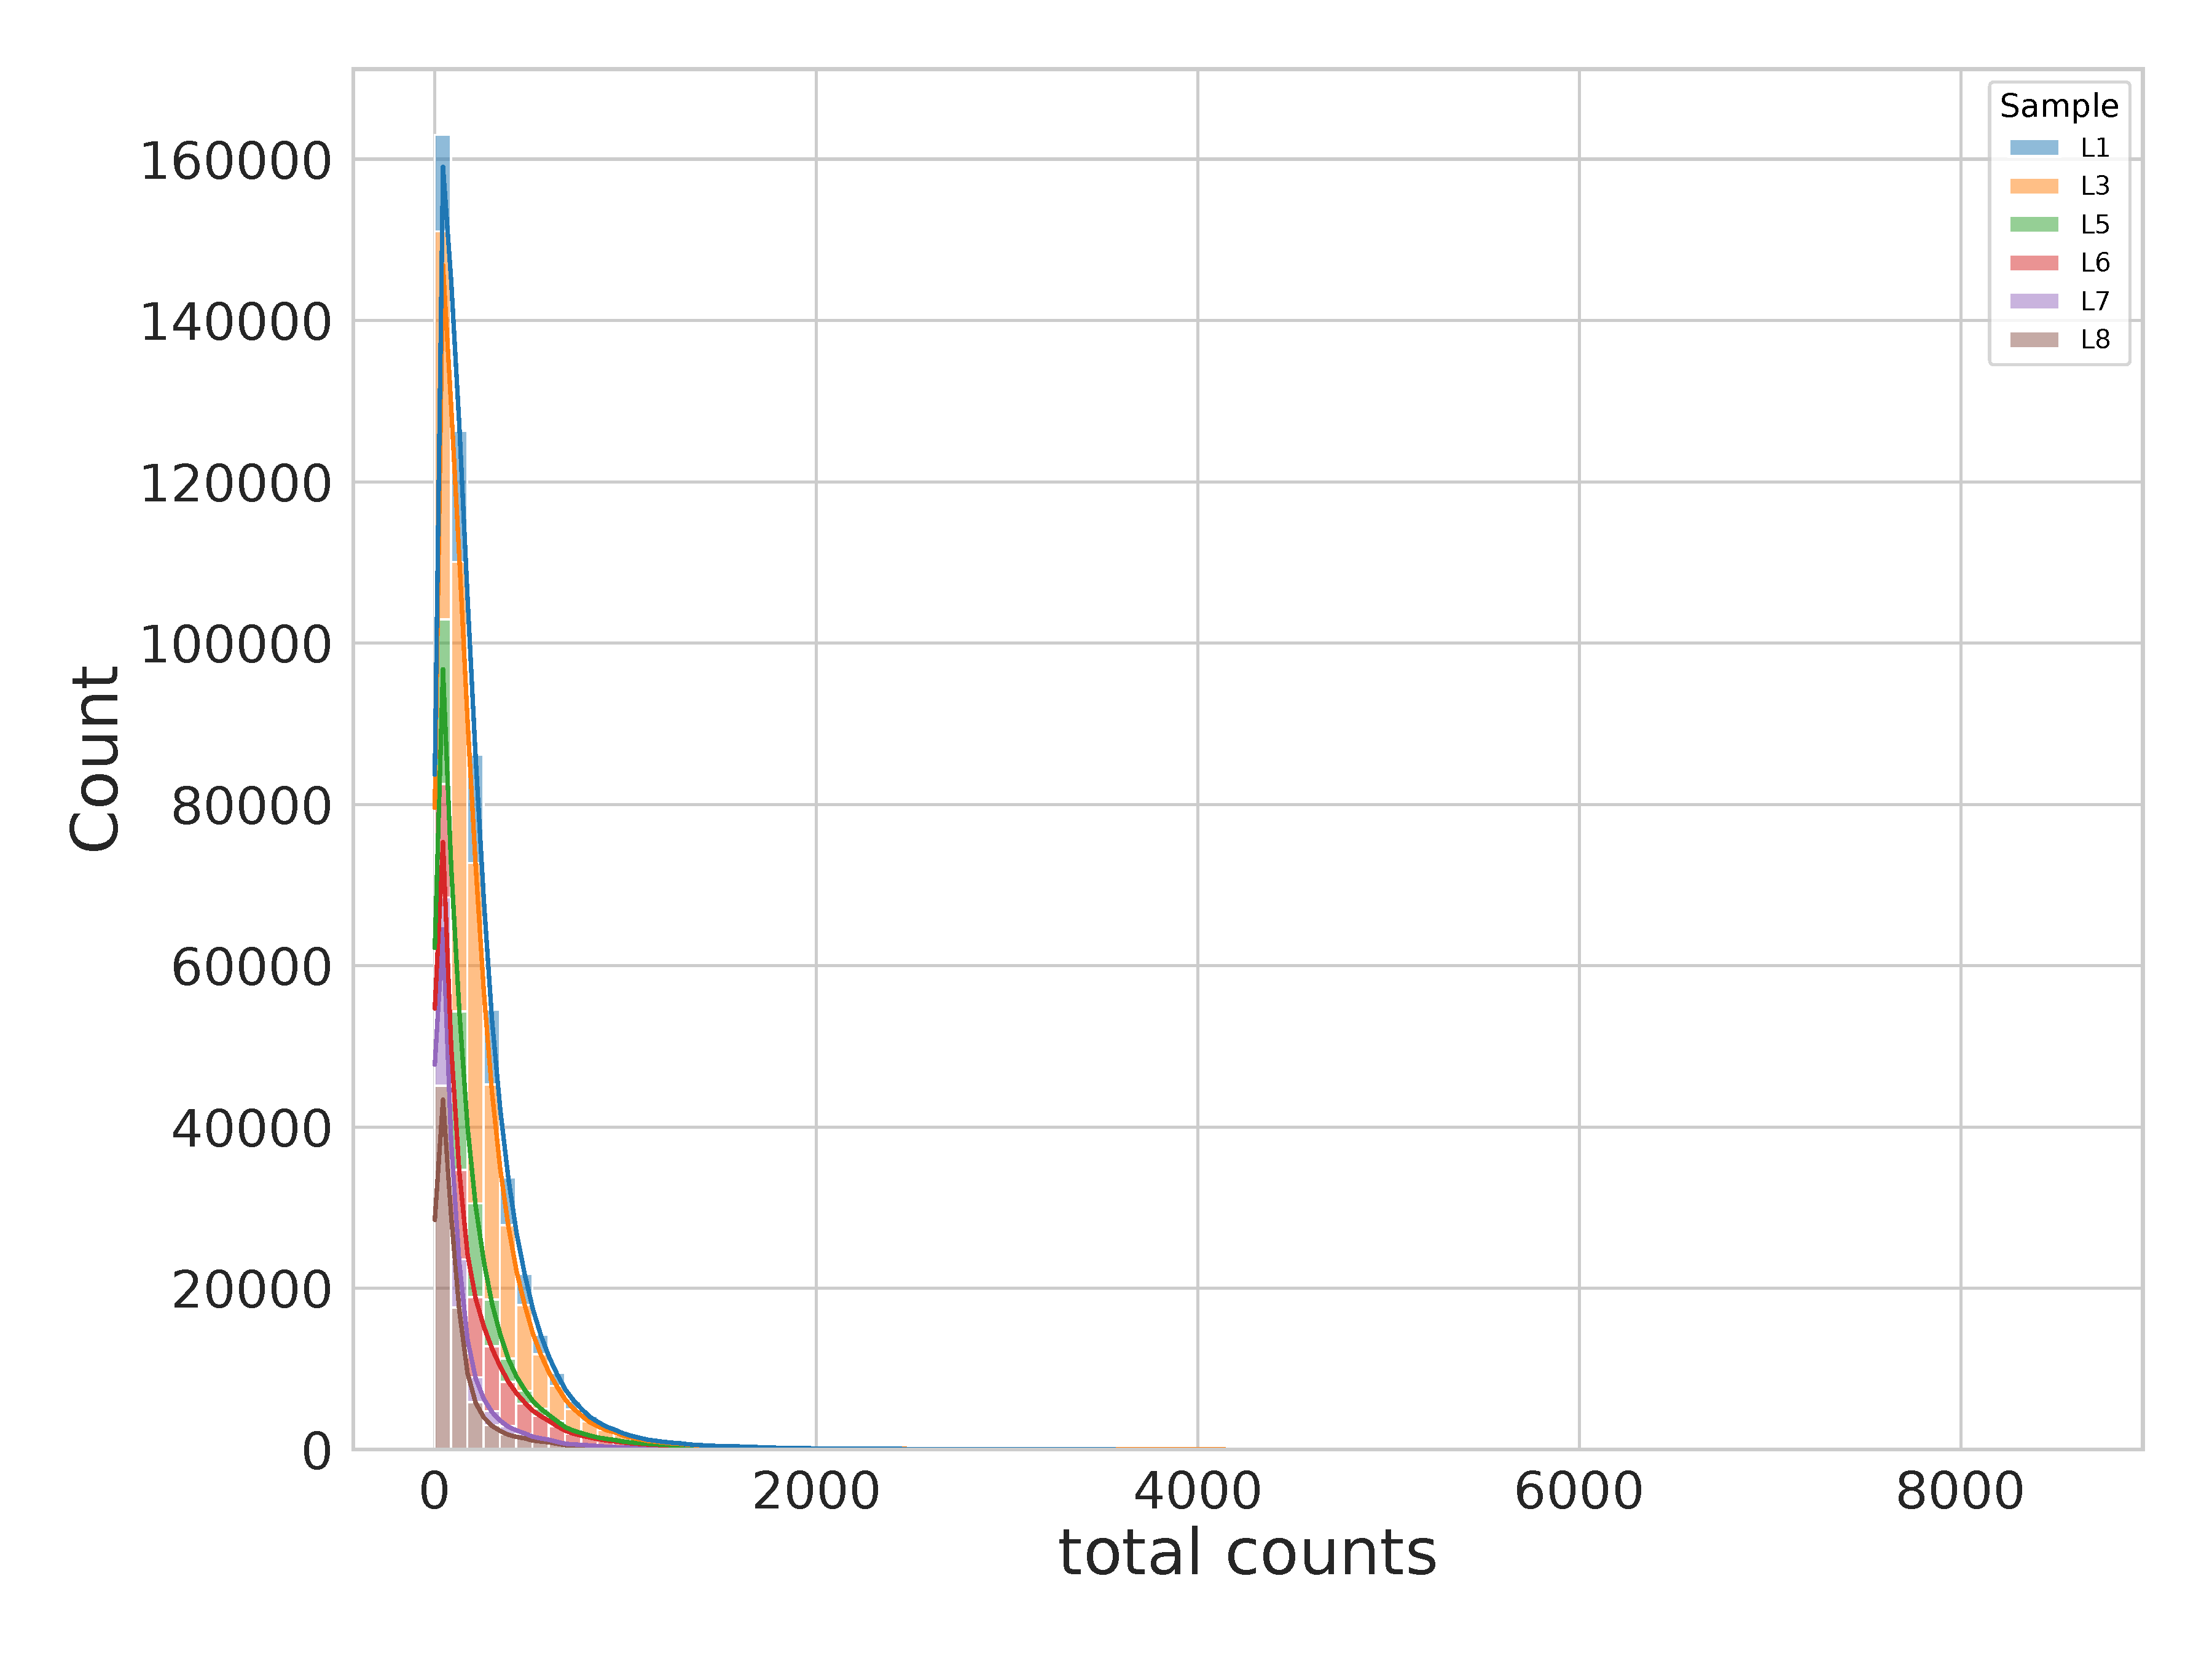
\includegraphics[width=\linewidth]{Figures/02_QC_expressed_genes/Cell-total_counts-Hist.pdf}
                        \caption{Total counts}
                    \end{figure}
                \end{column}
                \begin{column}{0.45 \textwidth}
                    \begin{figure}
                        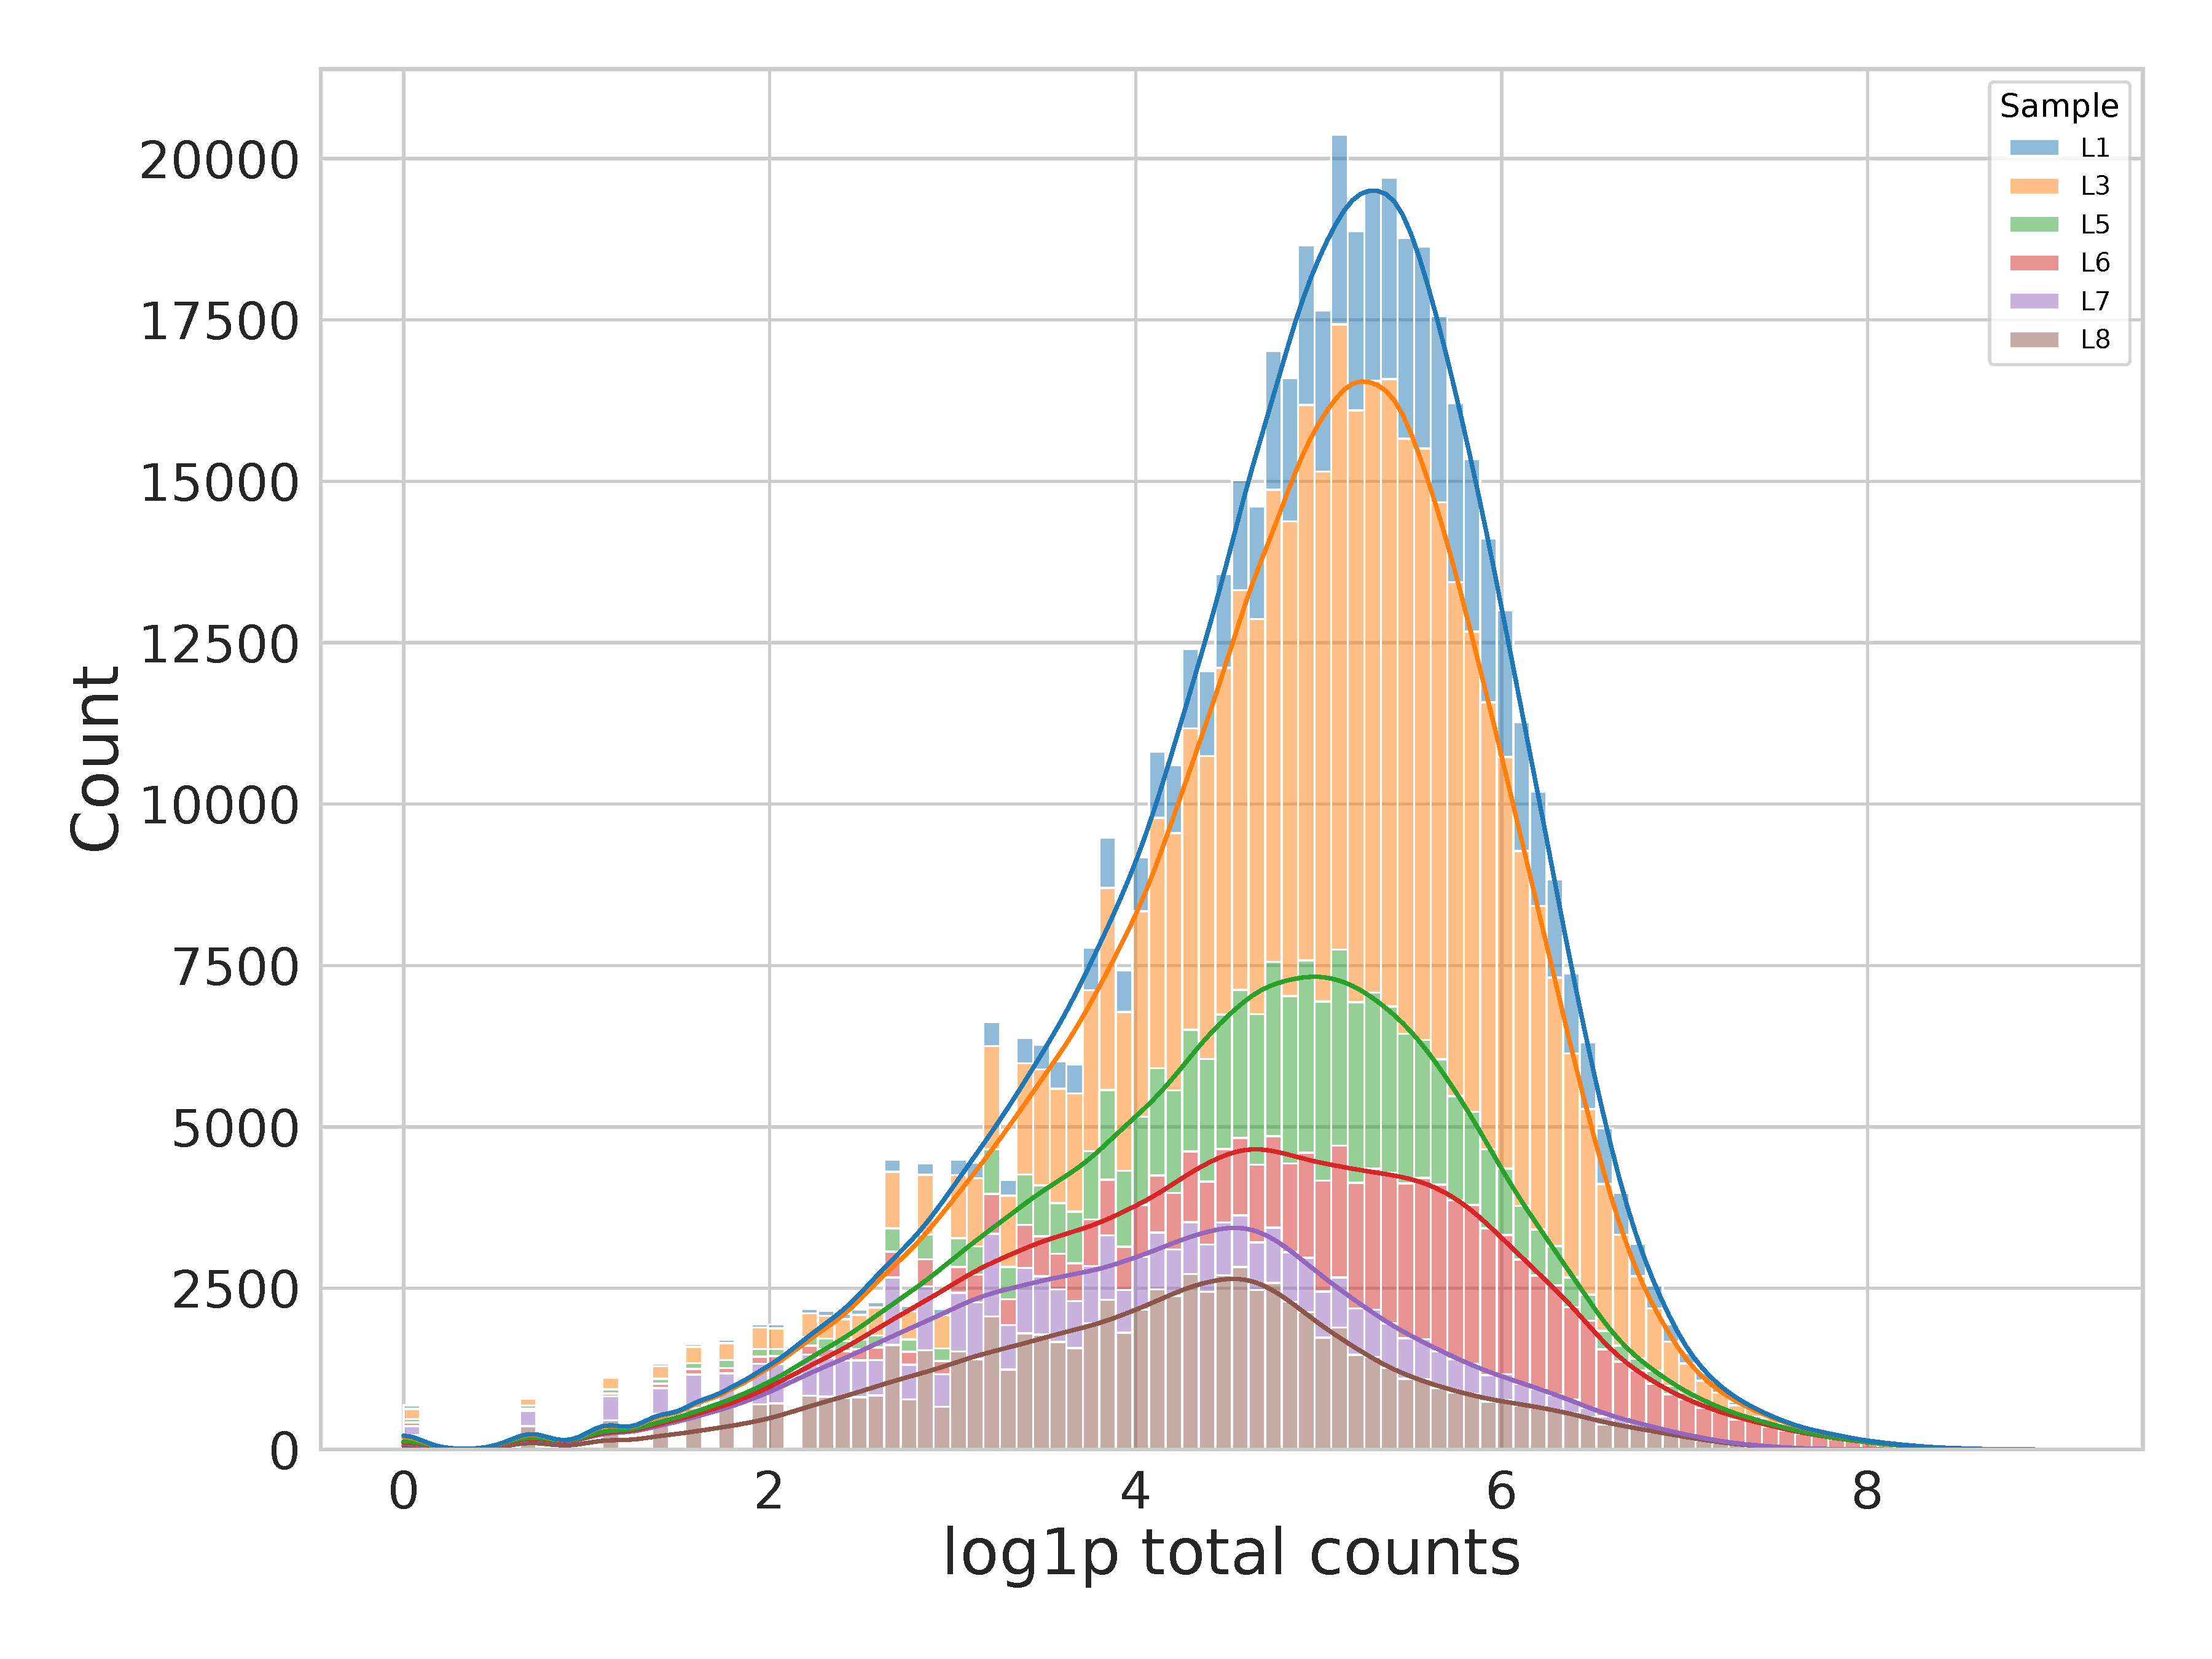
\includegraphics[width=\linewidth]{Figures/02_QC_expressed_genes/Cell-log1p_total_counts-Hist.pdf}
                        \caption{log1p(Total count)}
                    \end{figure}
                \end{column}
            \end{columns}
            \framebreak

            \begin{columns}
                \begin{column}{0.4 \textwidth}
                    \begin{figure}
                        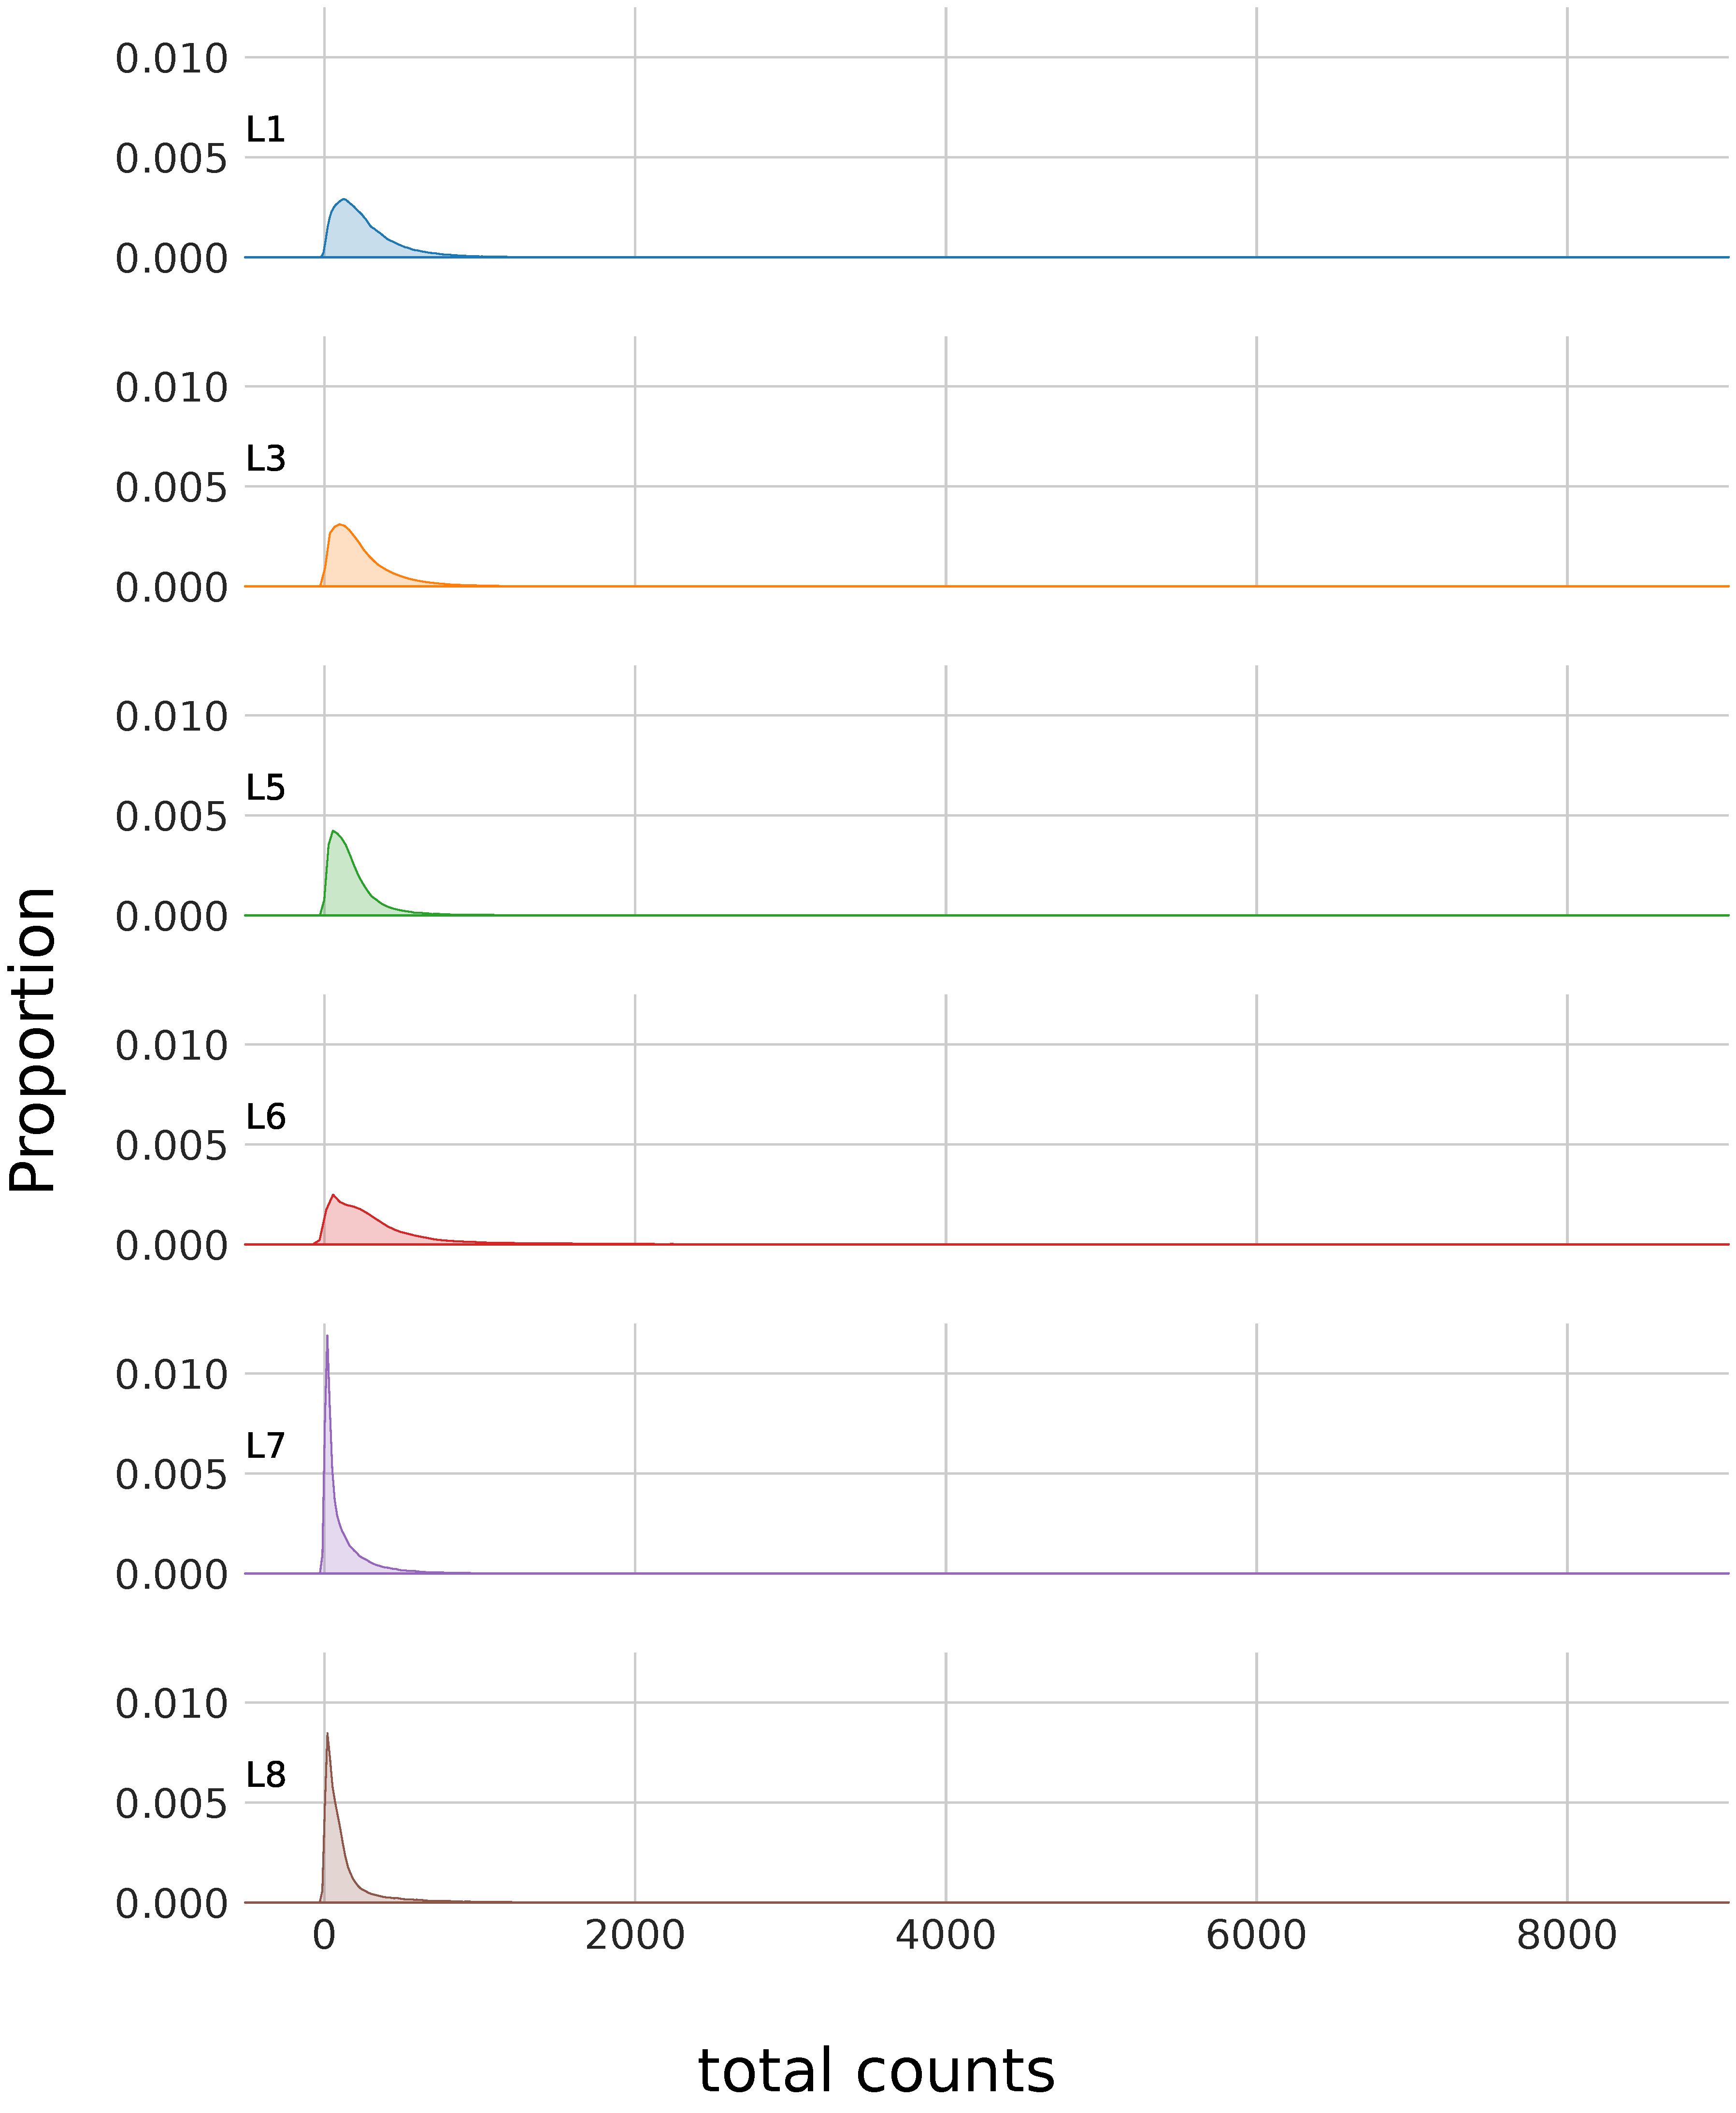
\includegraphics[width=\linewidth]{Figures/02_QC_expressed_genes/Cell-total_counts-HistMutiple.pdf}
                        \caption{Genes by counts}
                    \end{figure}
                \end{column}
                \begin{column}{0.4 \textwidth}
                    \begin{figure}
                        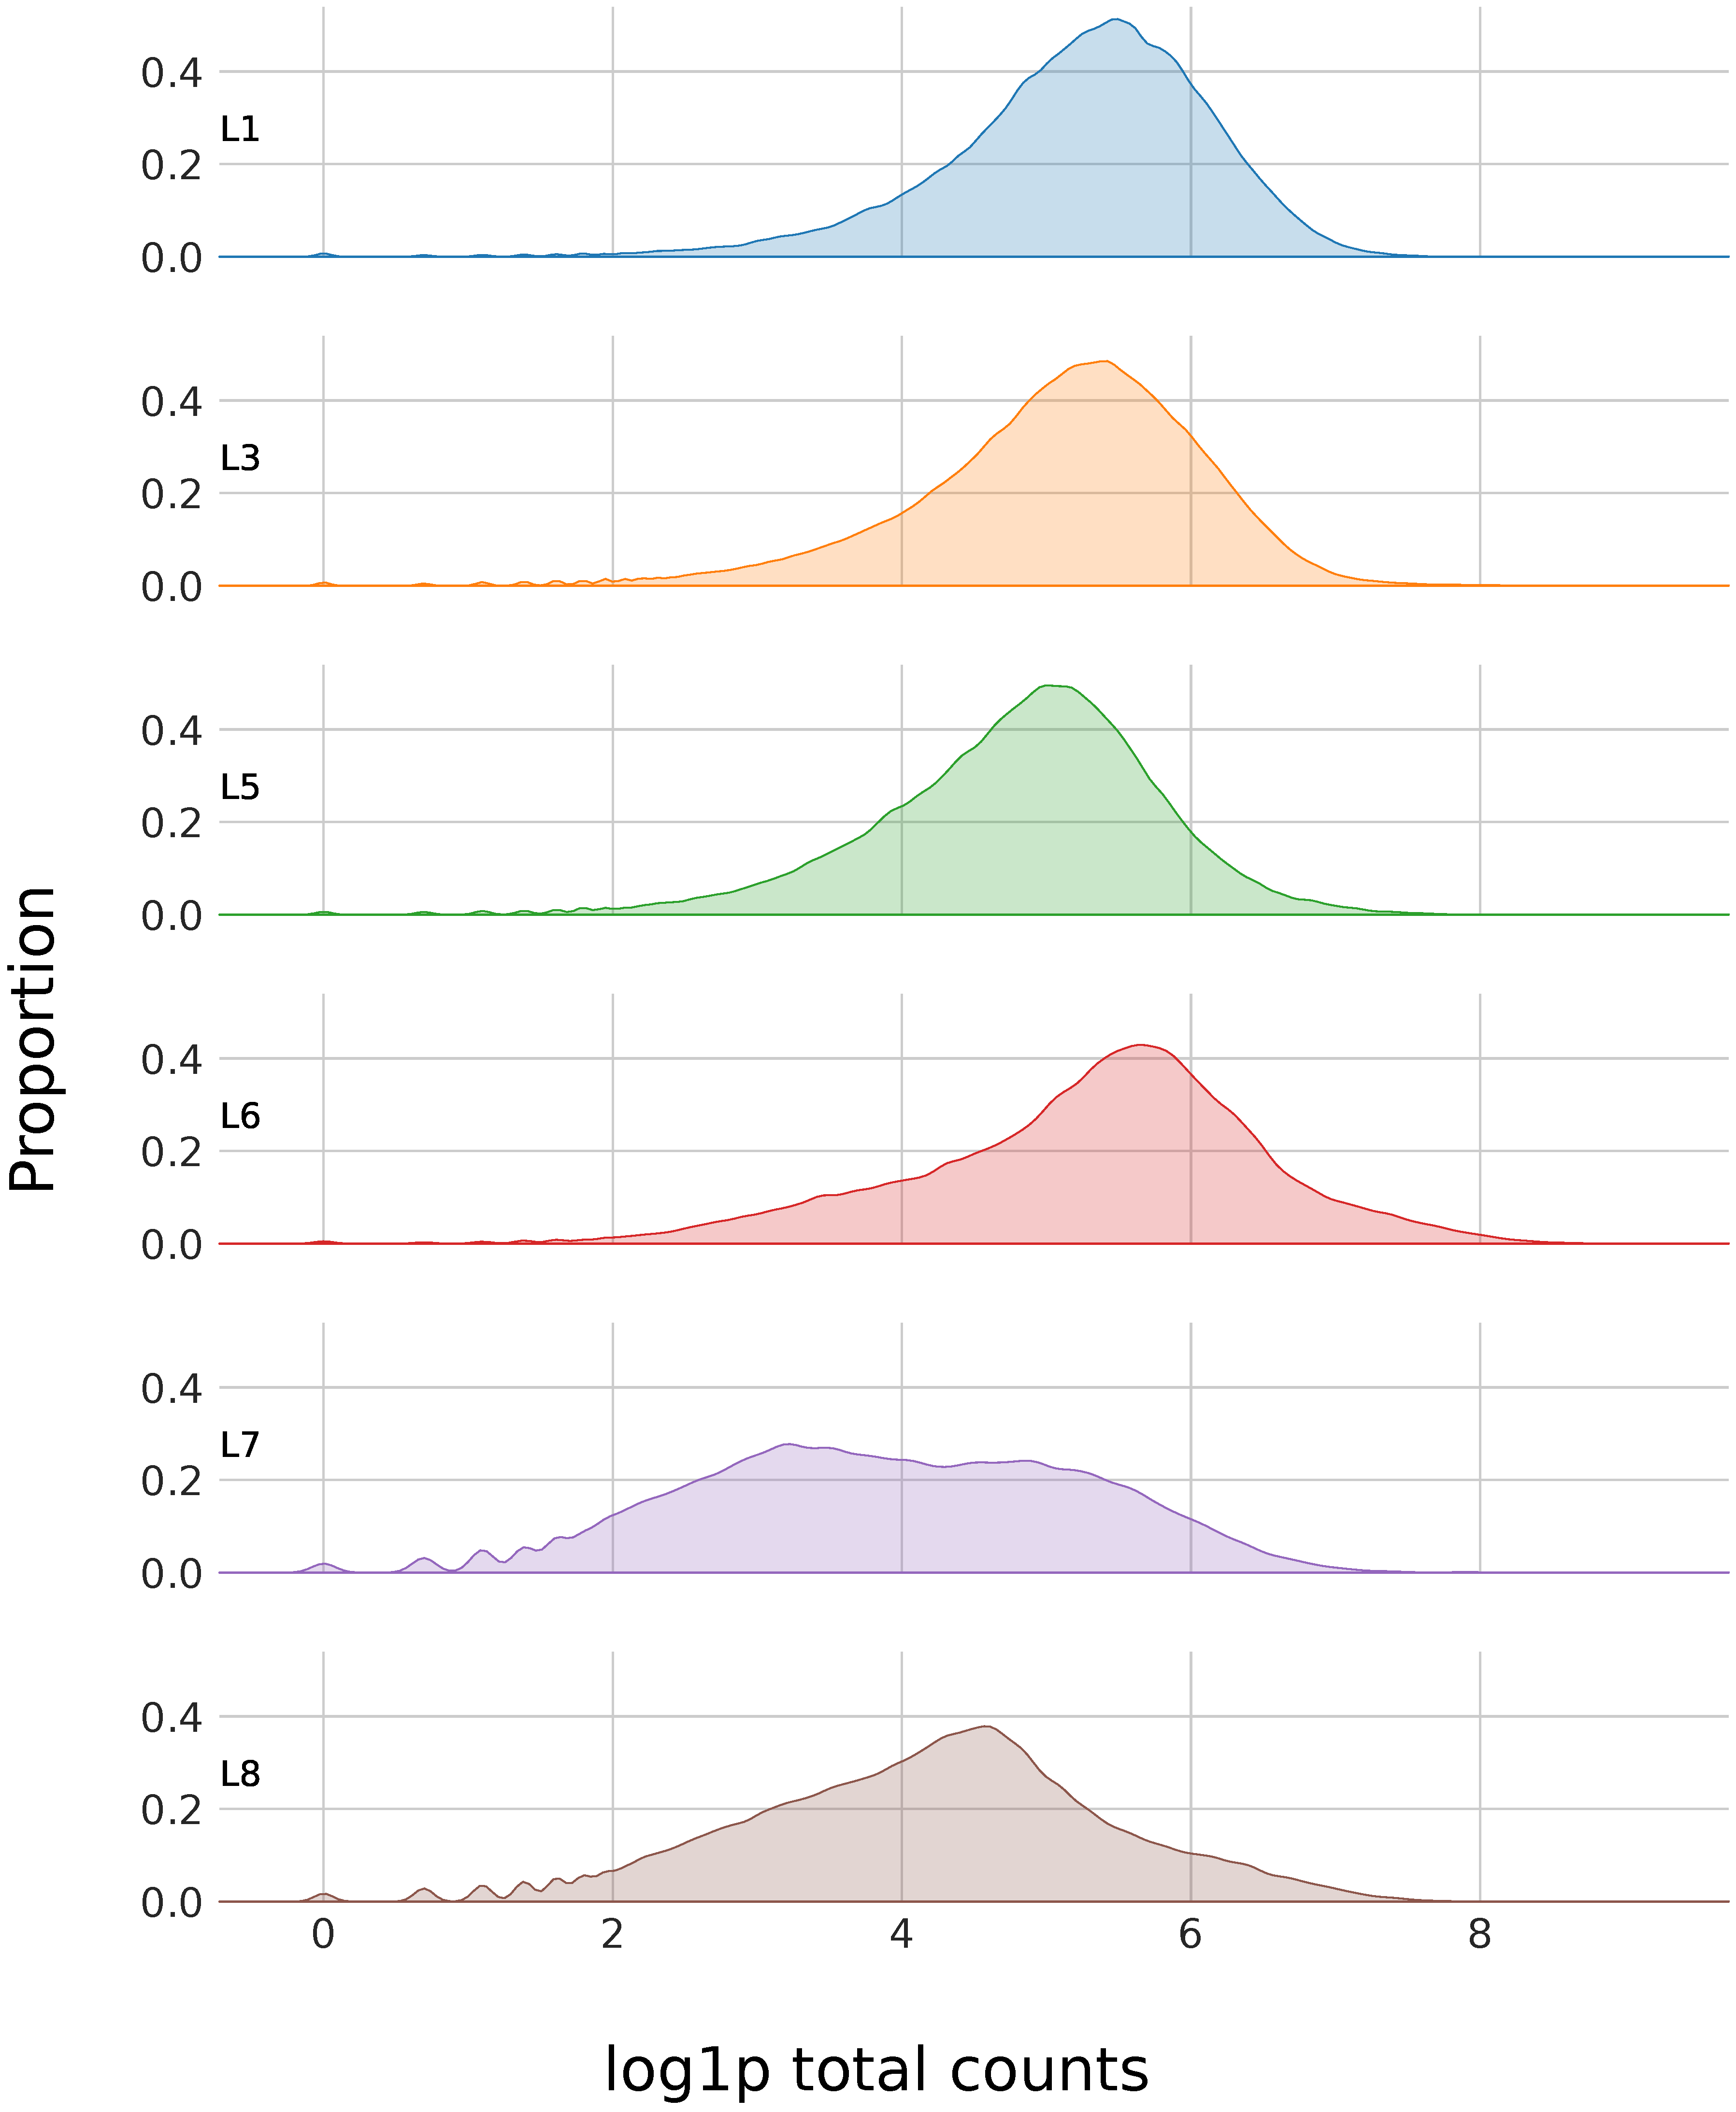
\includegraphics[width=\linewidth]{Figures/02_QC_expressed_genes/Cell-log1p_total_counts-HistMutiple.pdf}
                        \caption{log1p(Genes by count)}
                    \end{figure}
                \end{column}
            \end{columns}
            \framebreak

            \begin{columns}
                \begin{column}{0.45 \textwidth}
                    \begin{figure}
                        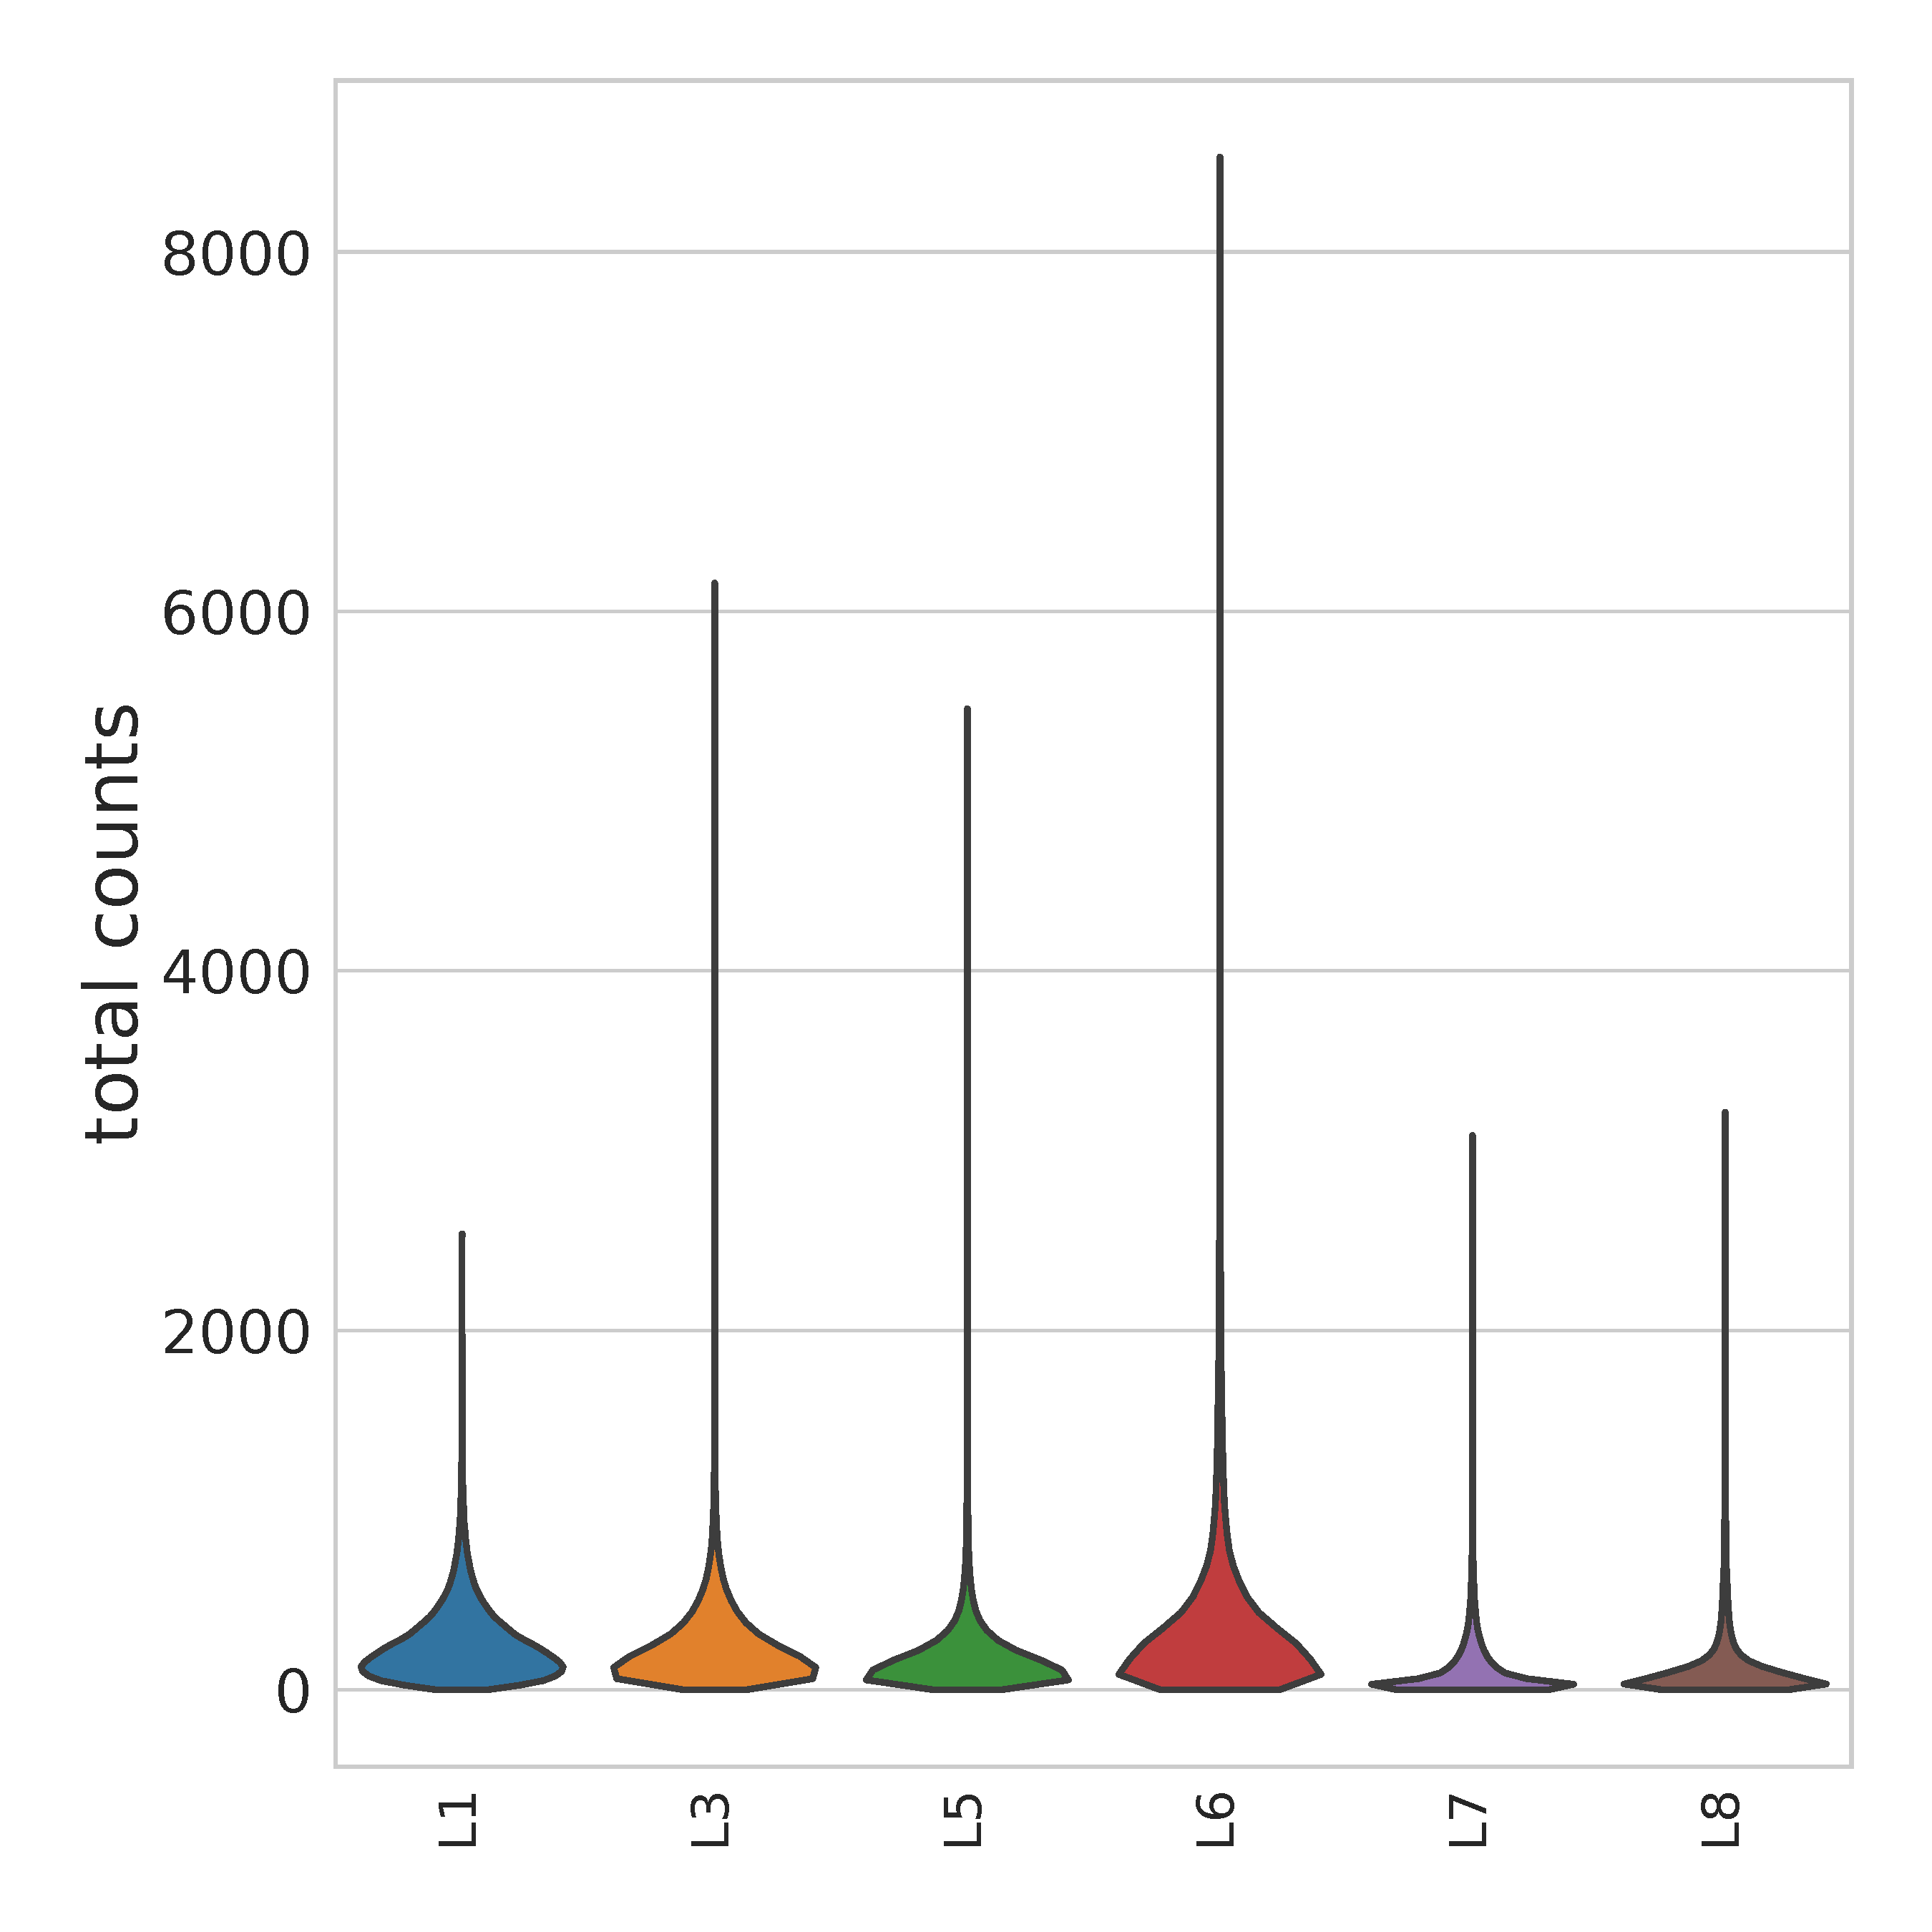
\includegraphics[width=\linewidth]{Figures/02_QC_expressed_genes/Cell-total_counts-Violin.pdf}
                        \caption{Genes by counts}
                    \end{figure}
                \end{column}
                \begin{column}{0.45 \textwidth}
                    \begin{figure}
                        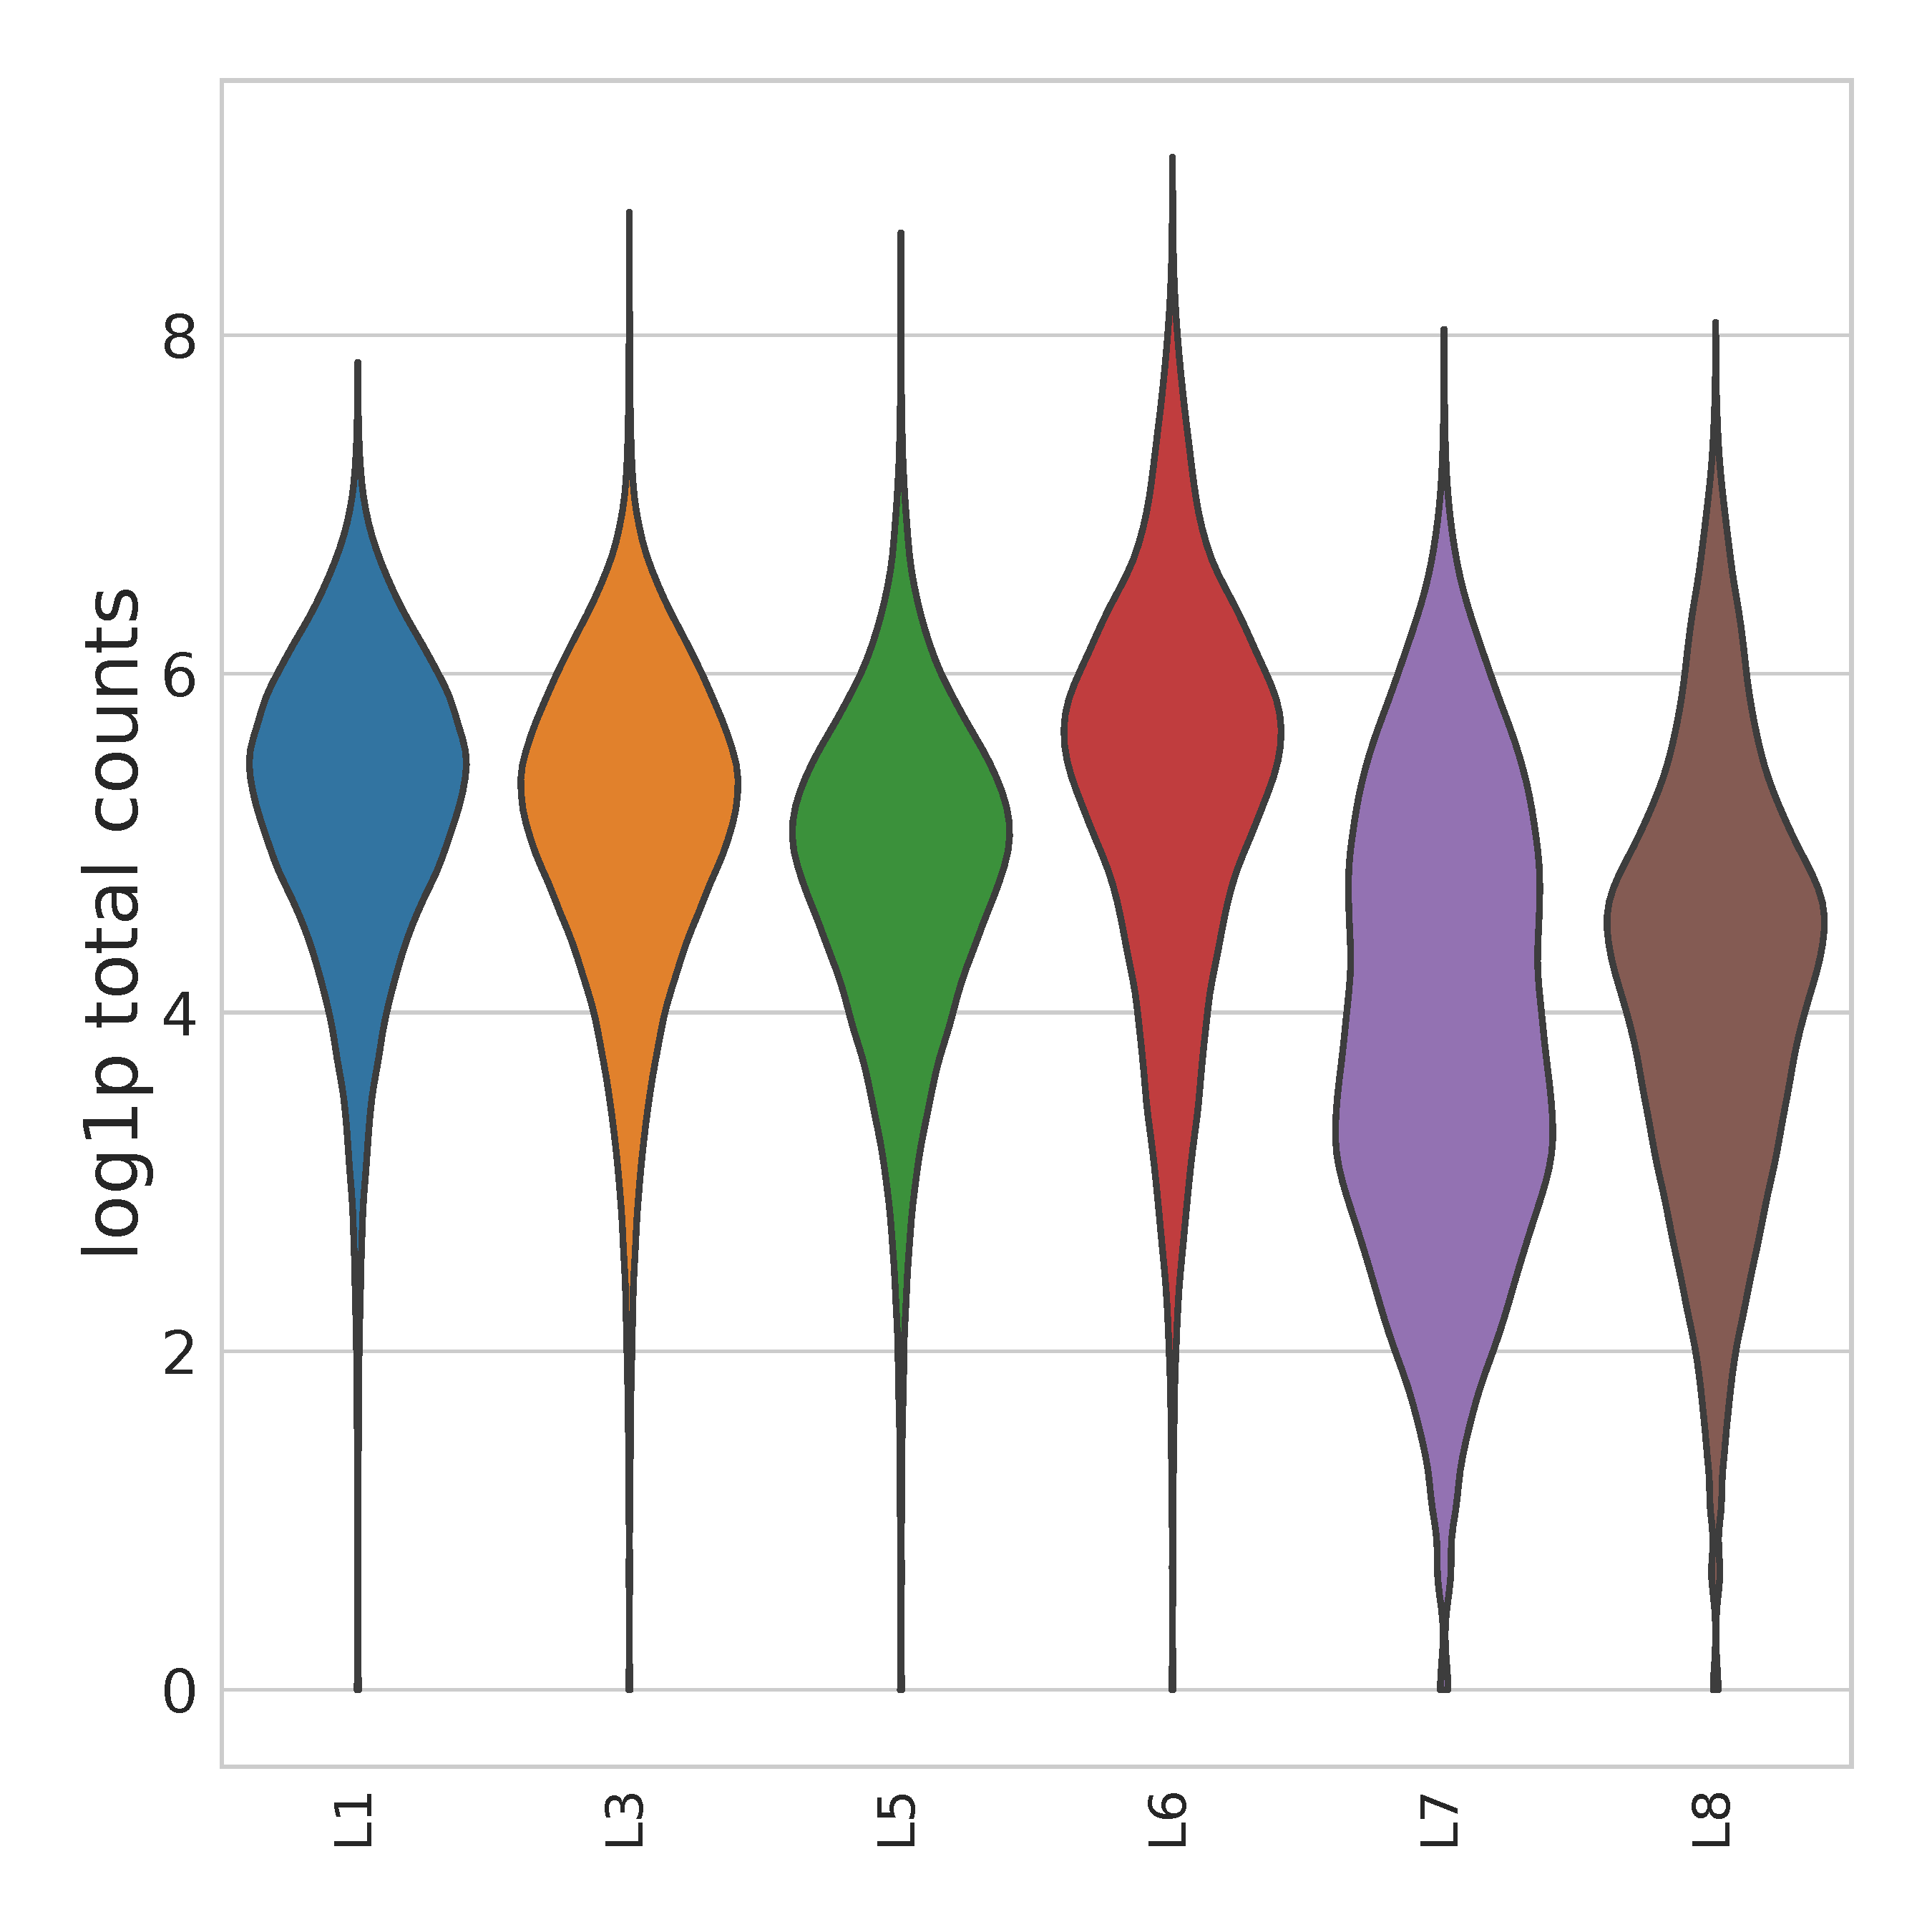
\includegraphics[width=\linewidth]{Figures/02_QC_expressed_genes/Cell-log1p_total_counts-Violin.pdf}
                        \caption{log1p(Genes by count)}
                    \end{figure}
                \end{column}
            \end{columns}
            \framebreak
        \end{frame}

        \begin{frame}[allowframebreaks]
            \frametitle{Genes by counts}

            \begin{columns}
                \begin{column}{0.45 \textwidth}
                    \begin{figure}
                        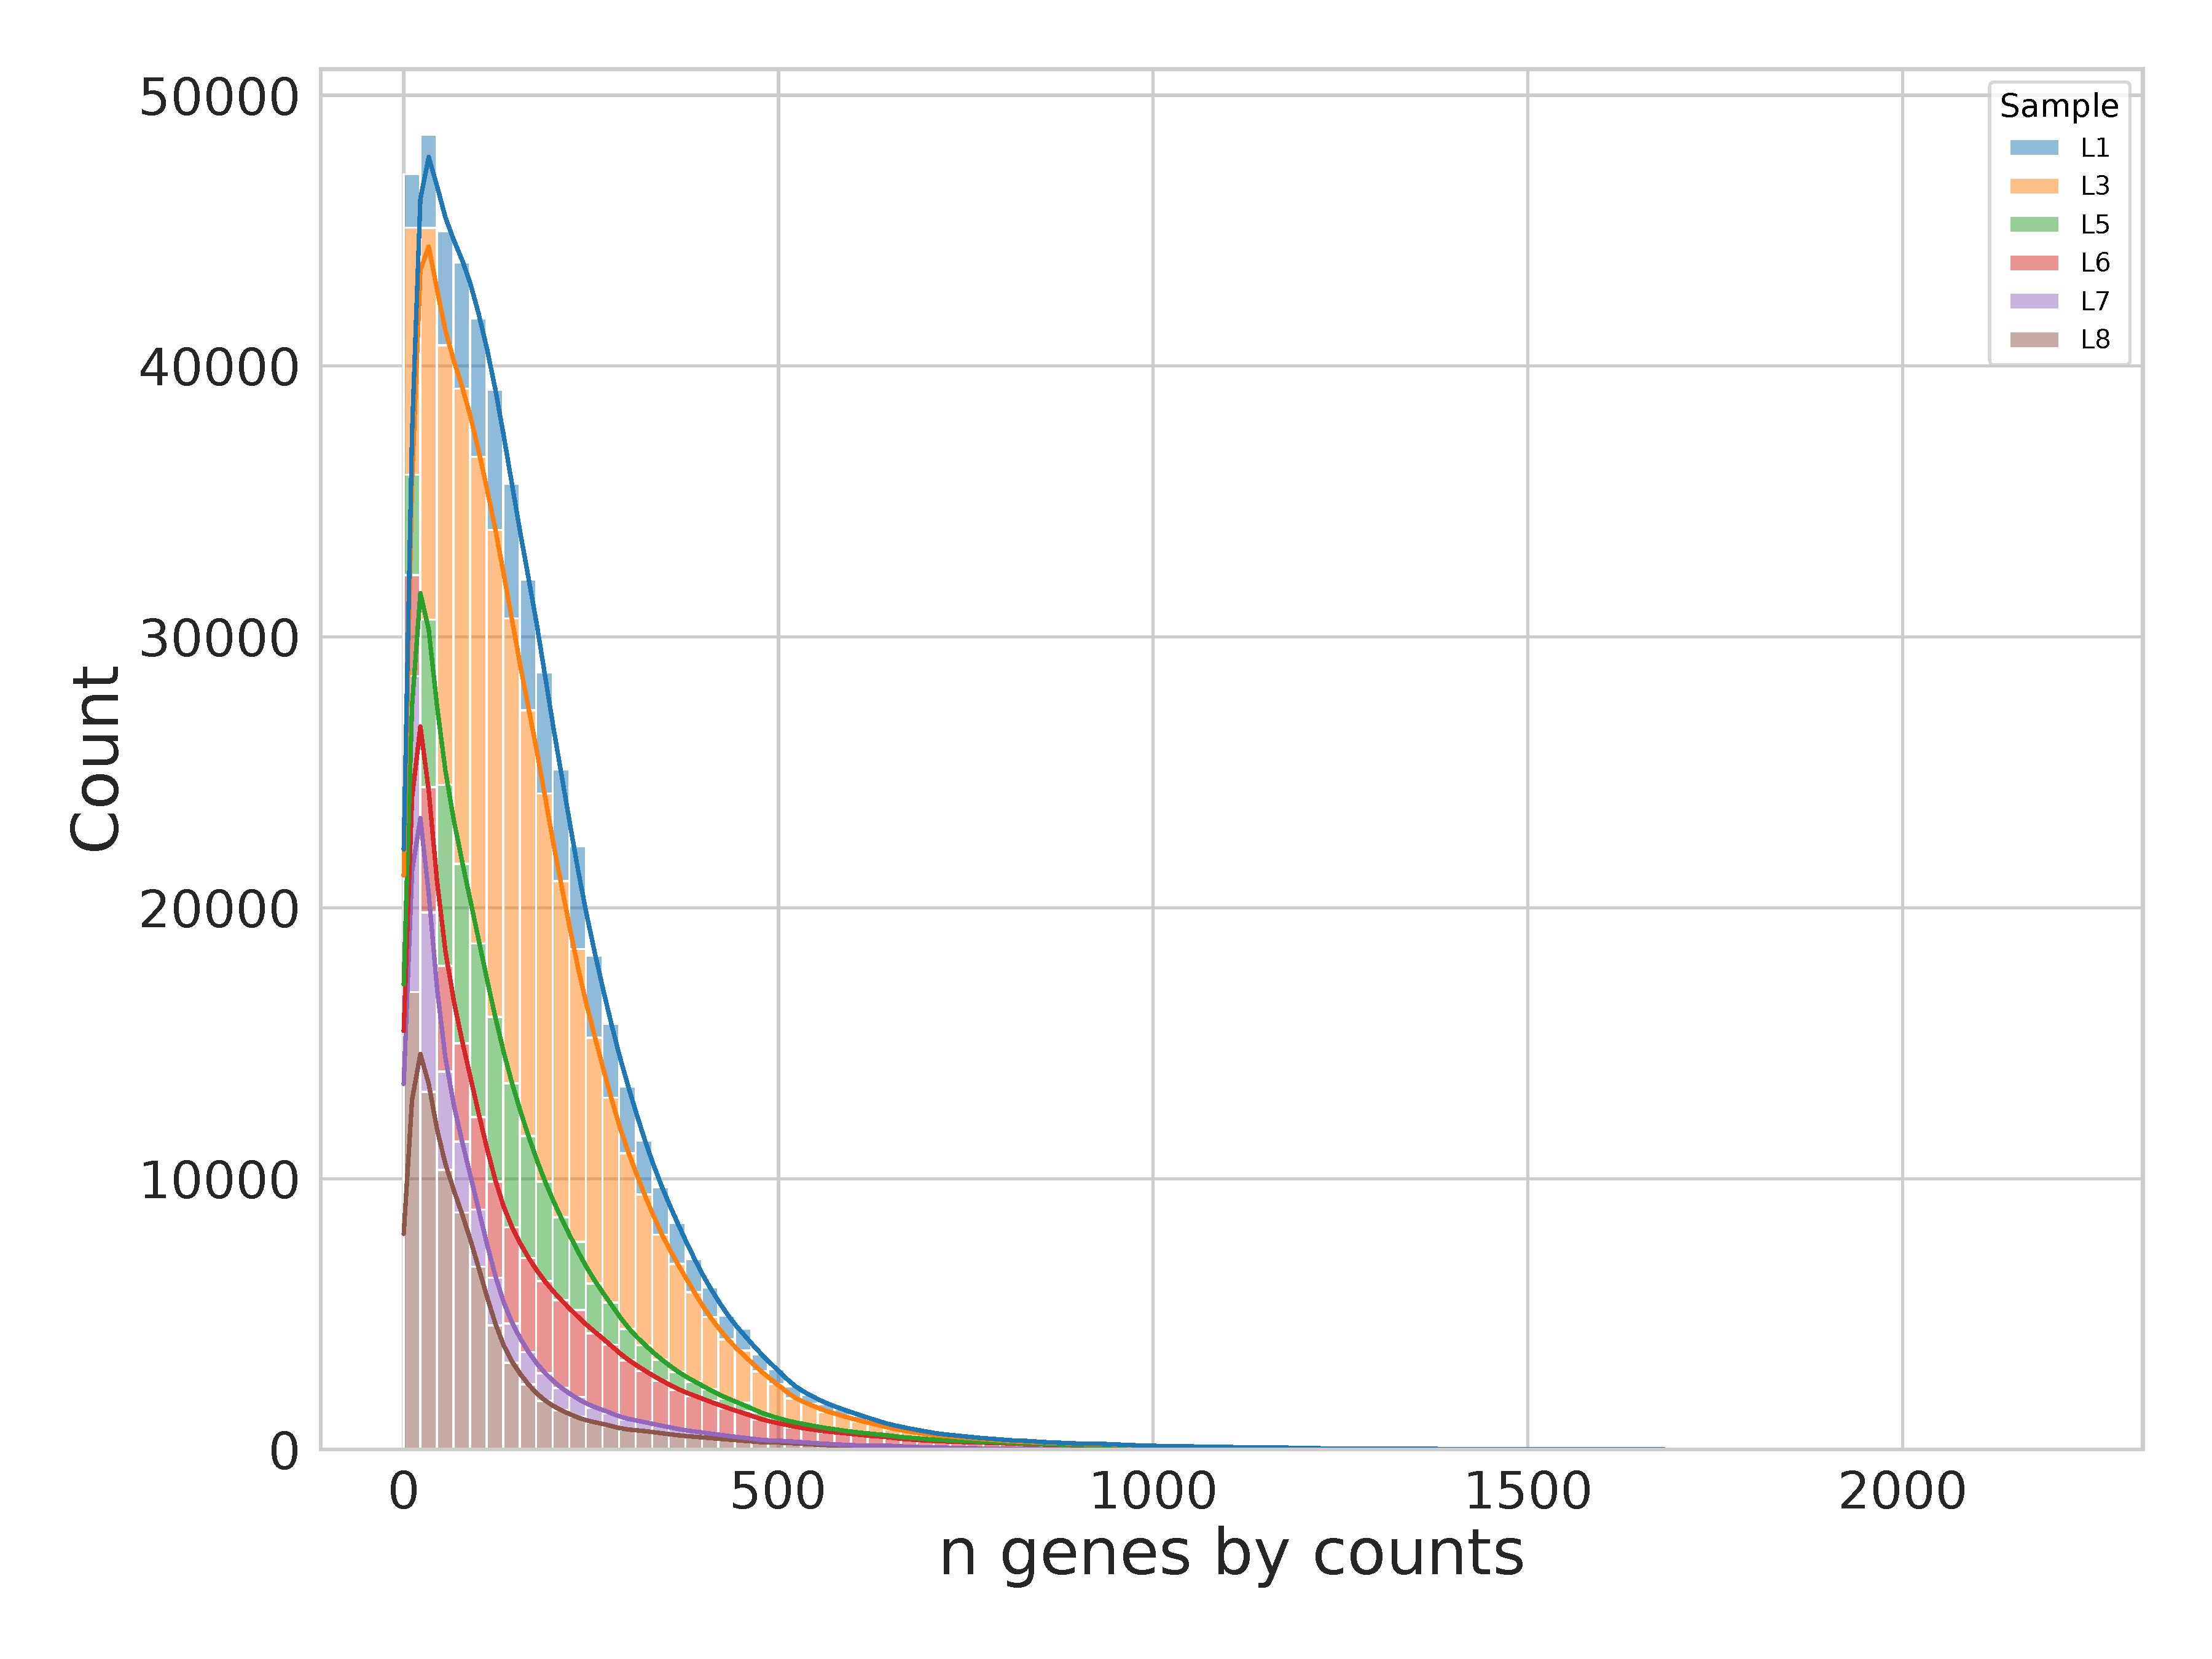
\includegraphics[width=\linewidth]{Figures/02_QC_expressed_genes/Cell-n_genes_by_counts-Hist.pdf}
                        \caption{Genes by counts}
                    \end{figure}
                \end{column}
                \begin{column}{0.45 \textwidth}
                    \begin{figure}
                        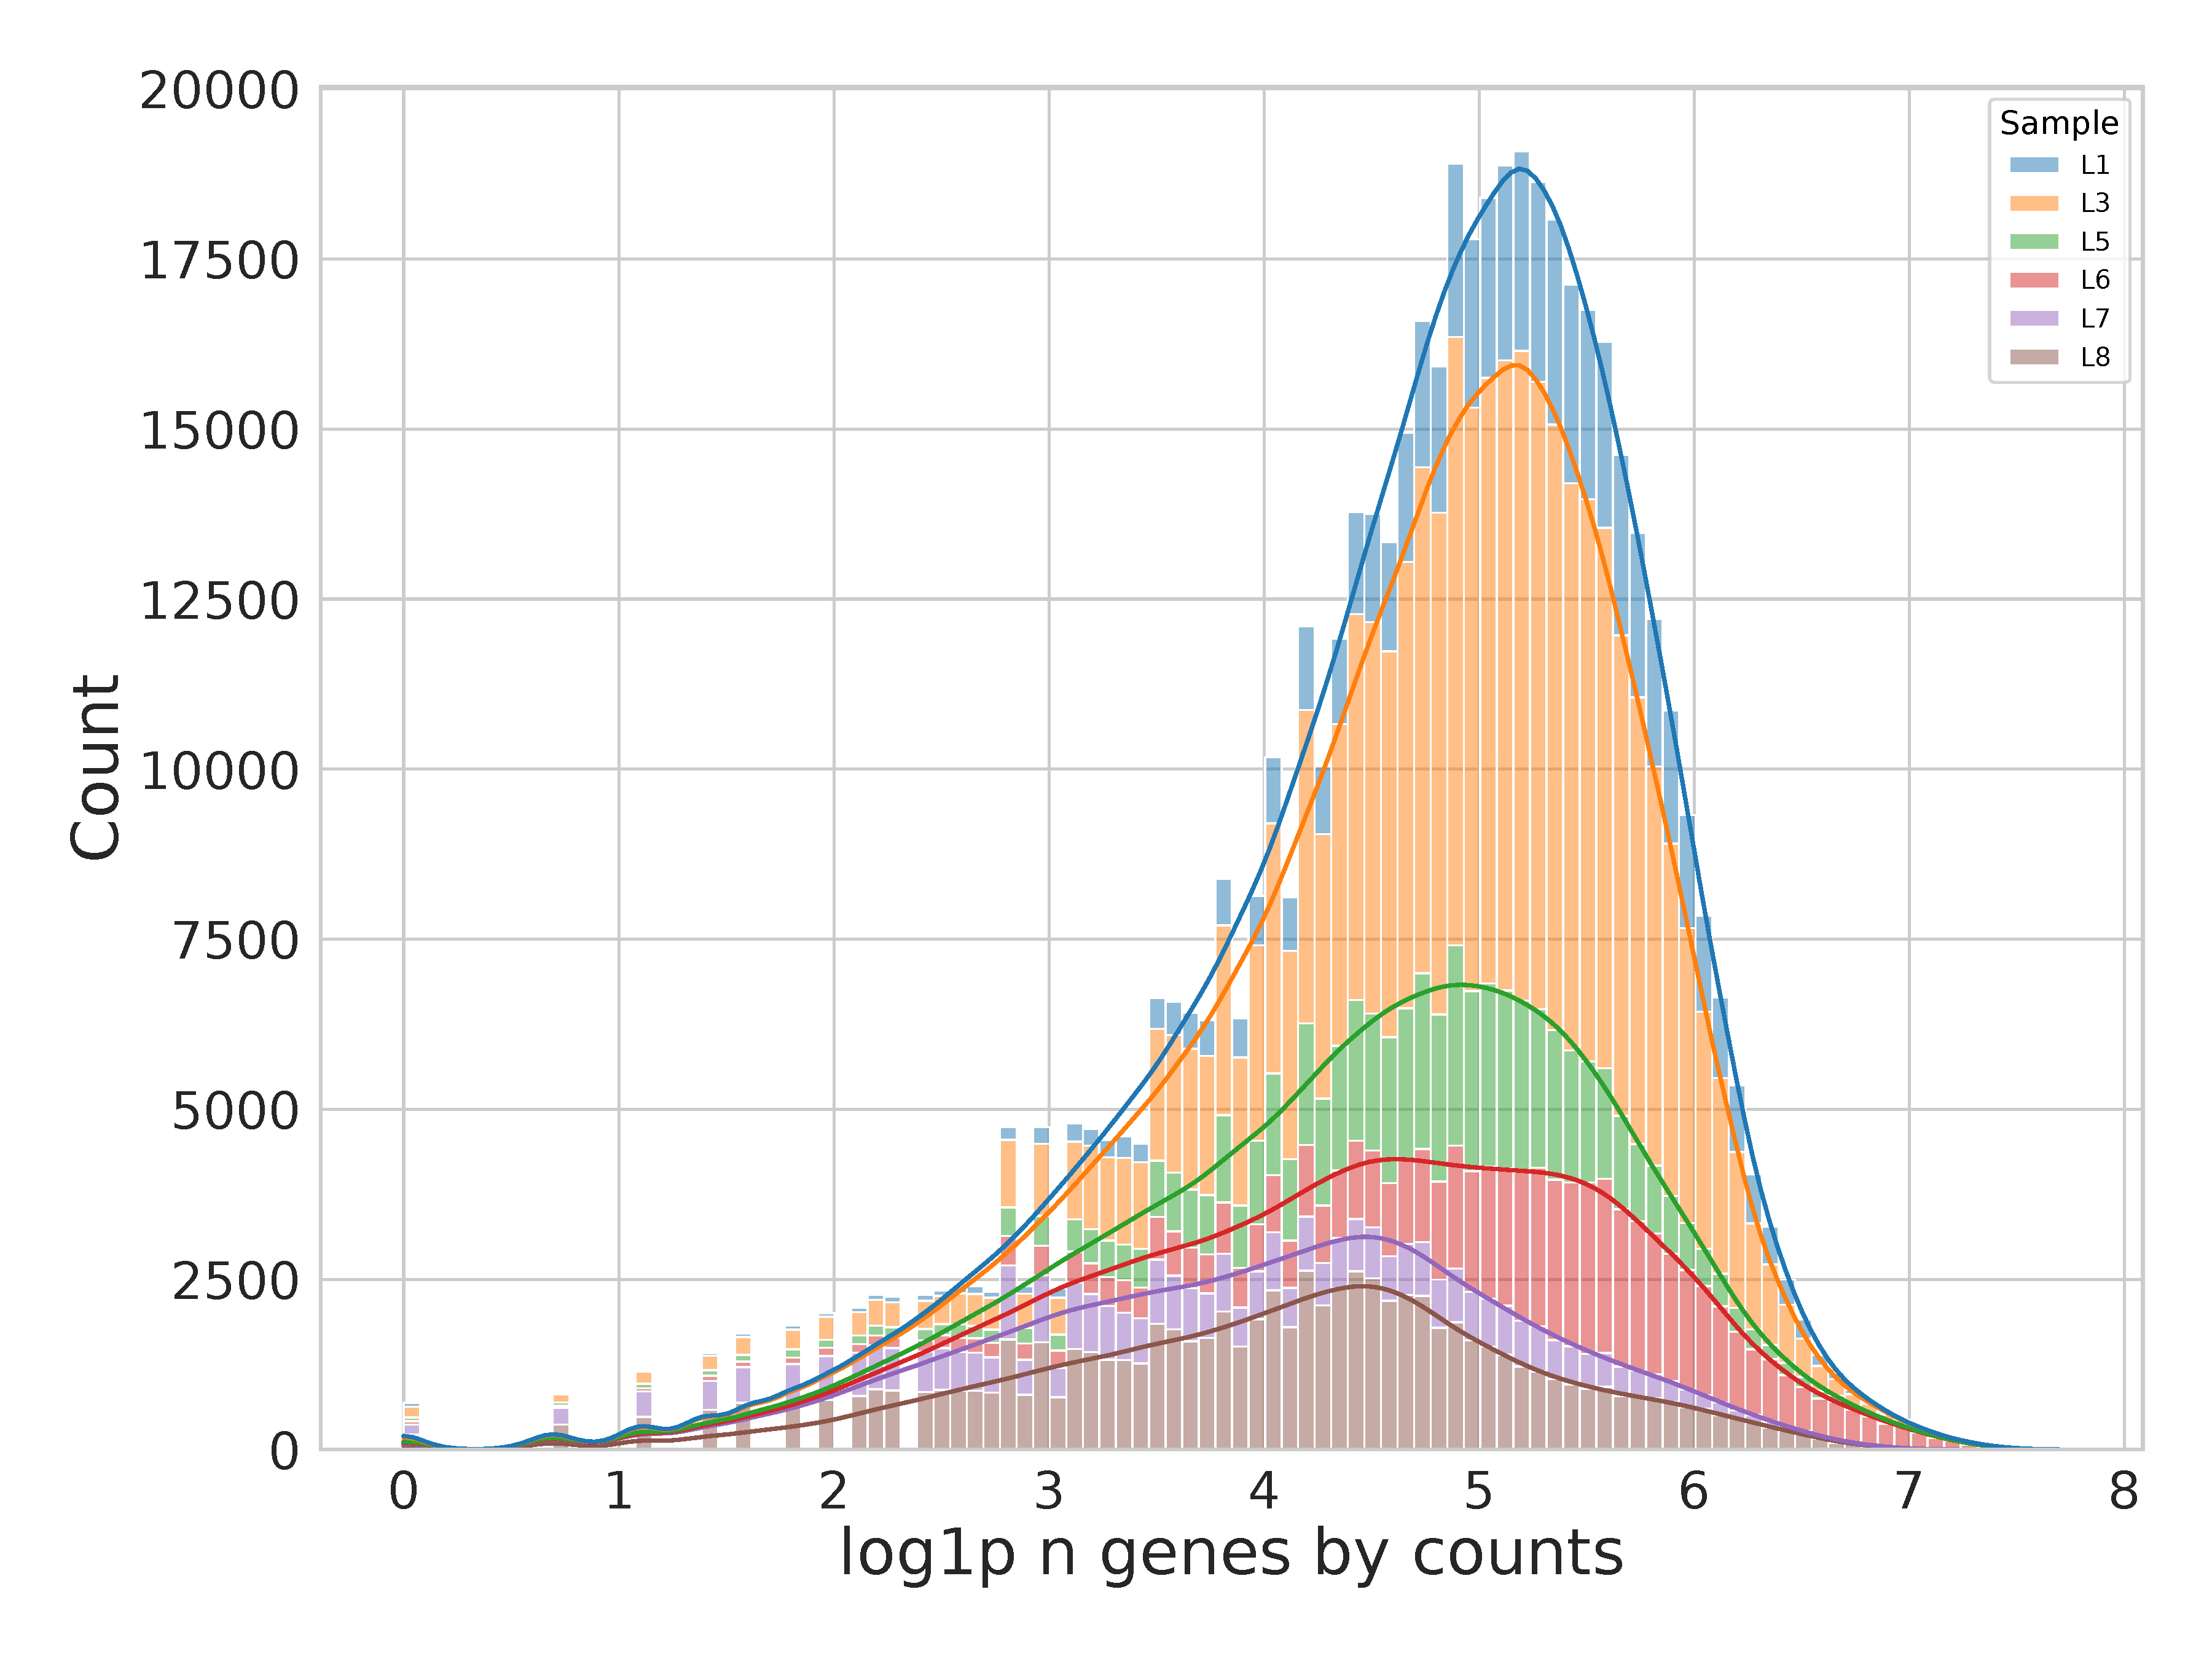
\includegraphics[width=\linewidth]{Figures/02_QC_expressed_genes/Cell-log1p_n_genes_by_counts-Hist.pdf}
                        \caption{log1p(Genes by count)}
                    \end{figure}
                \end{column}
            \end{columns}
            \framebreak

            \begin{columns}
                \begin{column}{0.4 \textwidth}
                    \begin{figure}
                        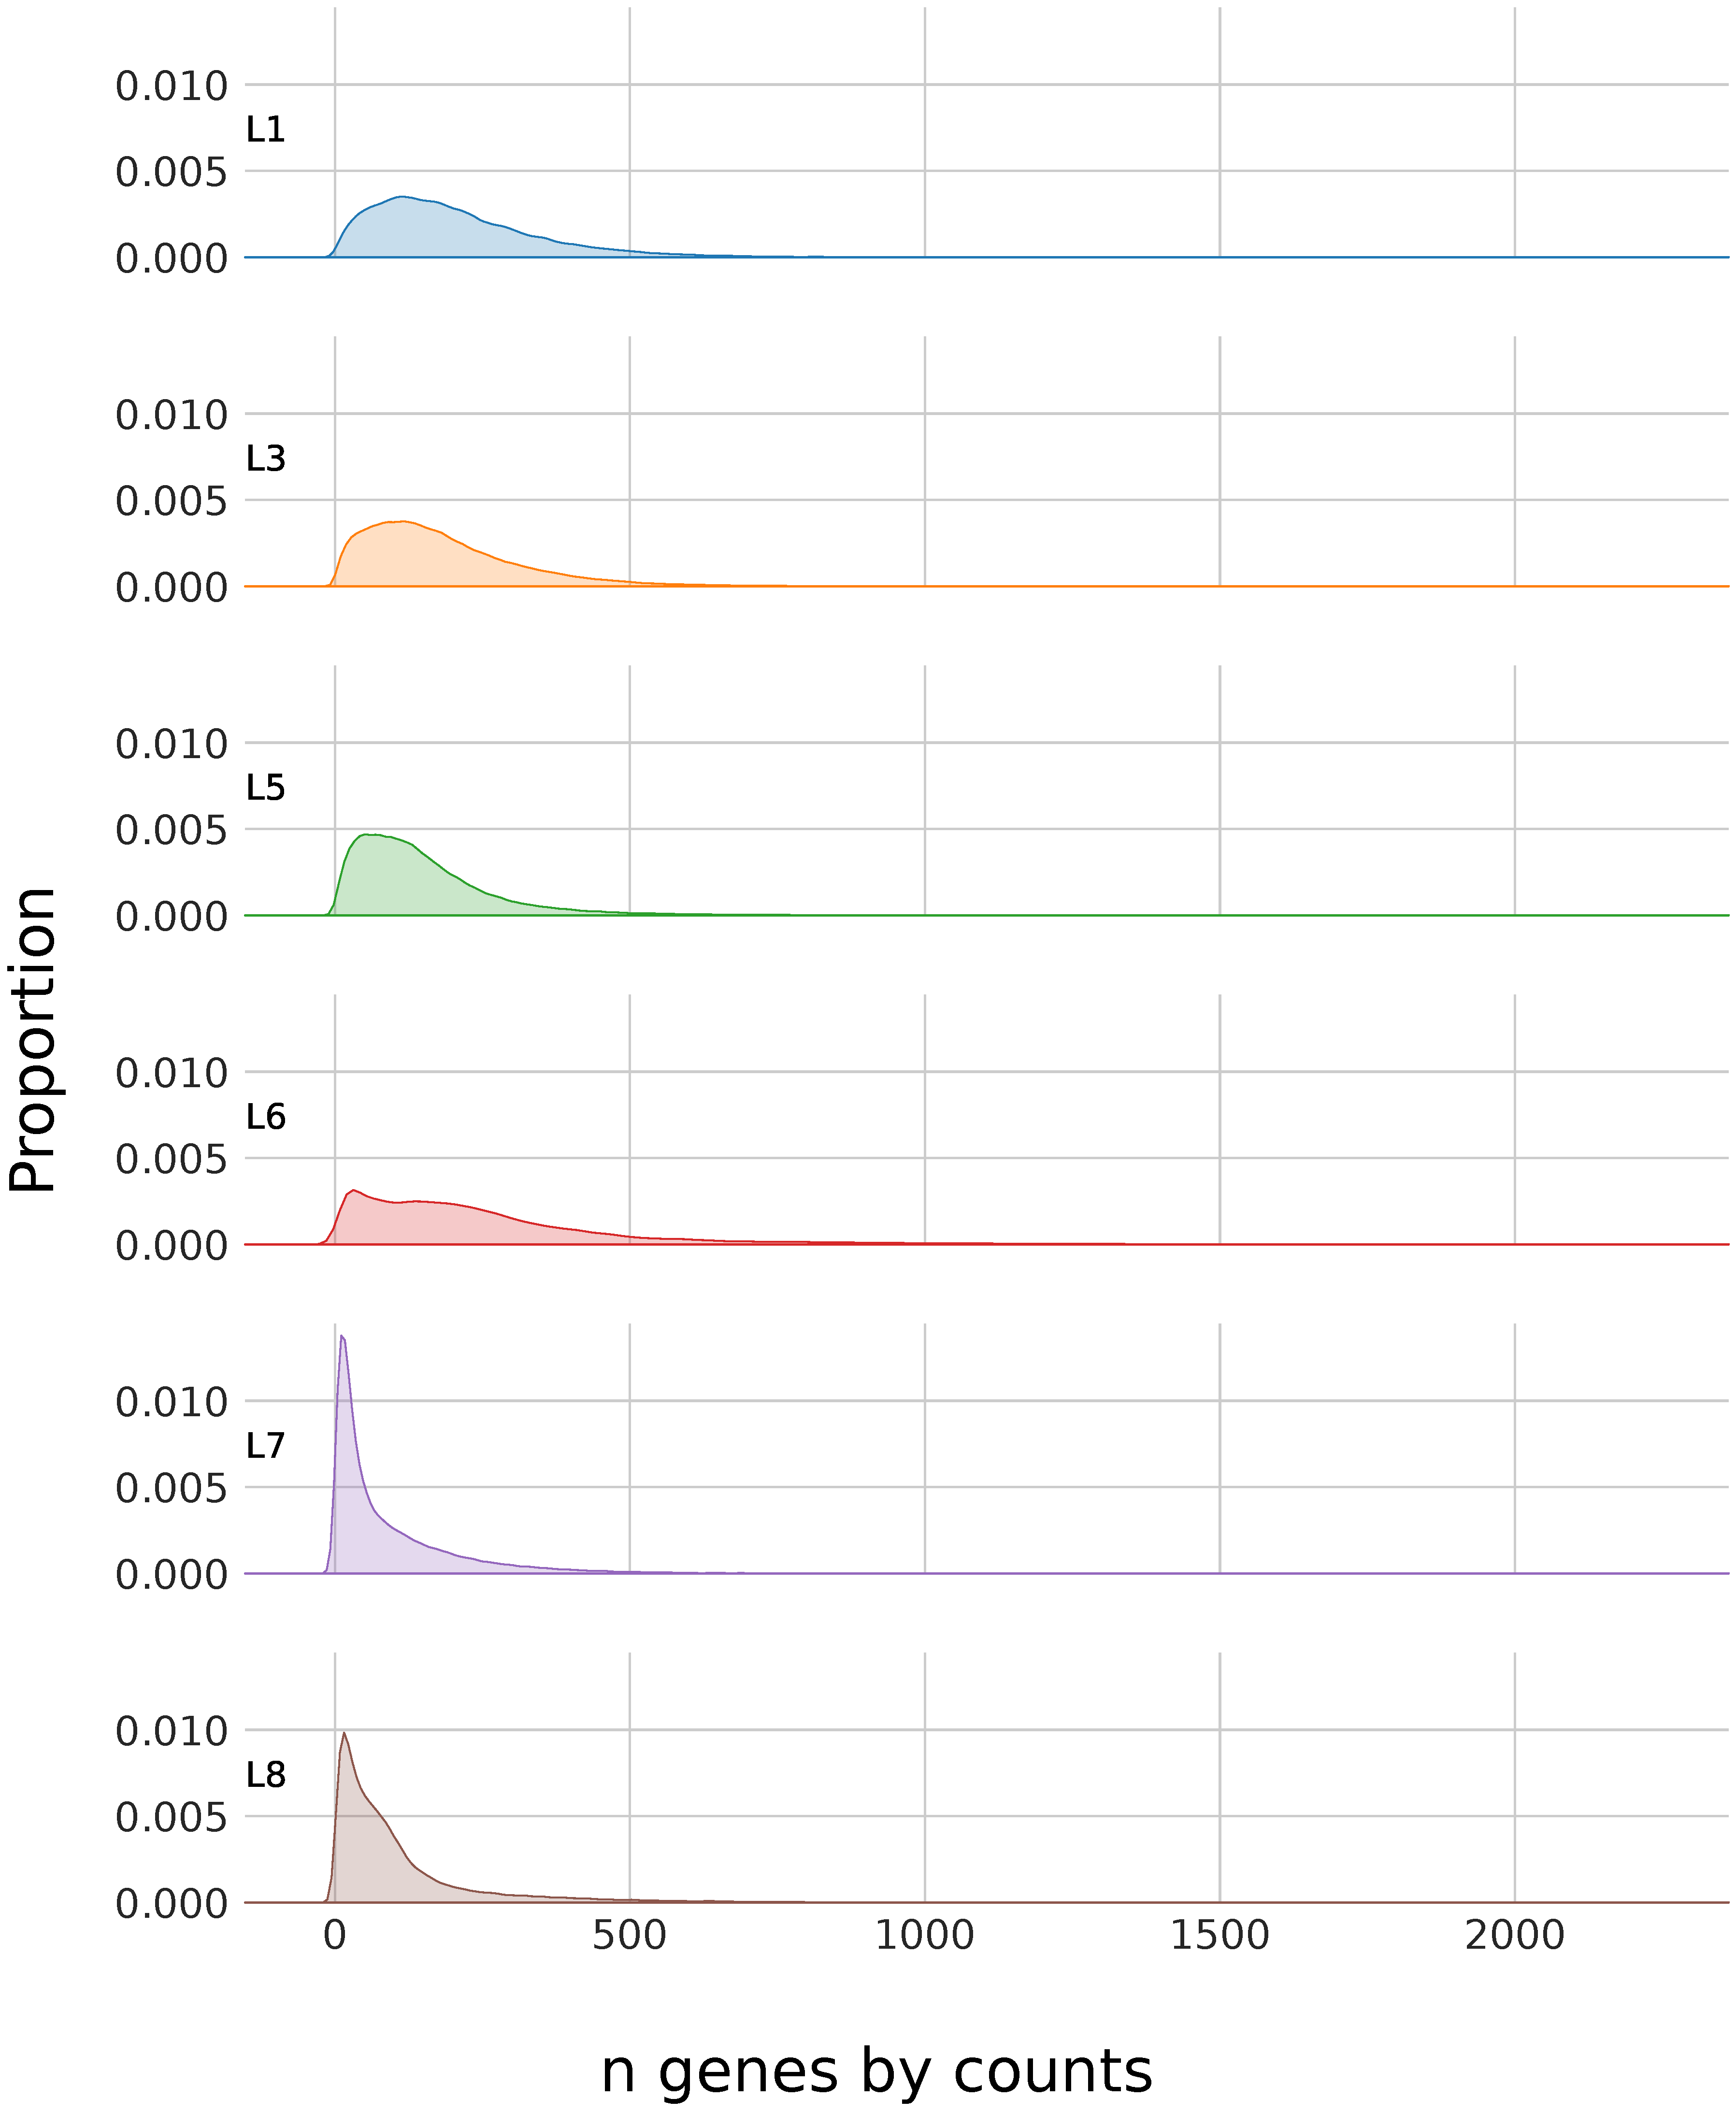
\includegraphics[width=\linewidth]{Figures/02_QC_expressed_genes/Cell-n_genes_by_counts-HistMutiple.pdf}
                        \caption{Genes by counts}
                    \end{figure}
                \end{column}
                \begin{column}{0.4 \textwidth}
                    \begin{figure}
                        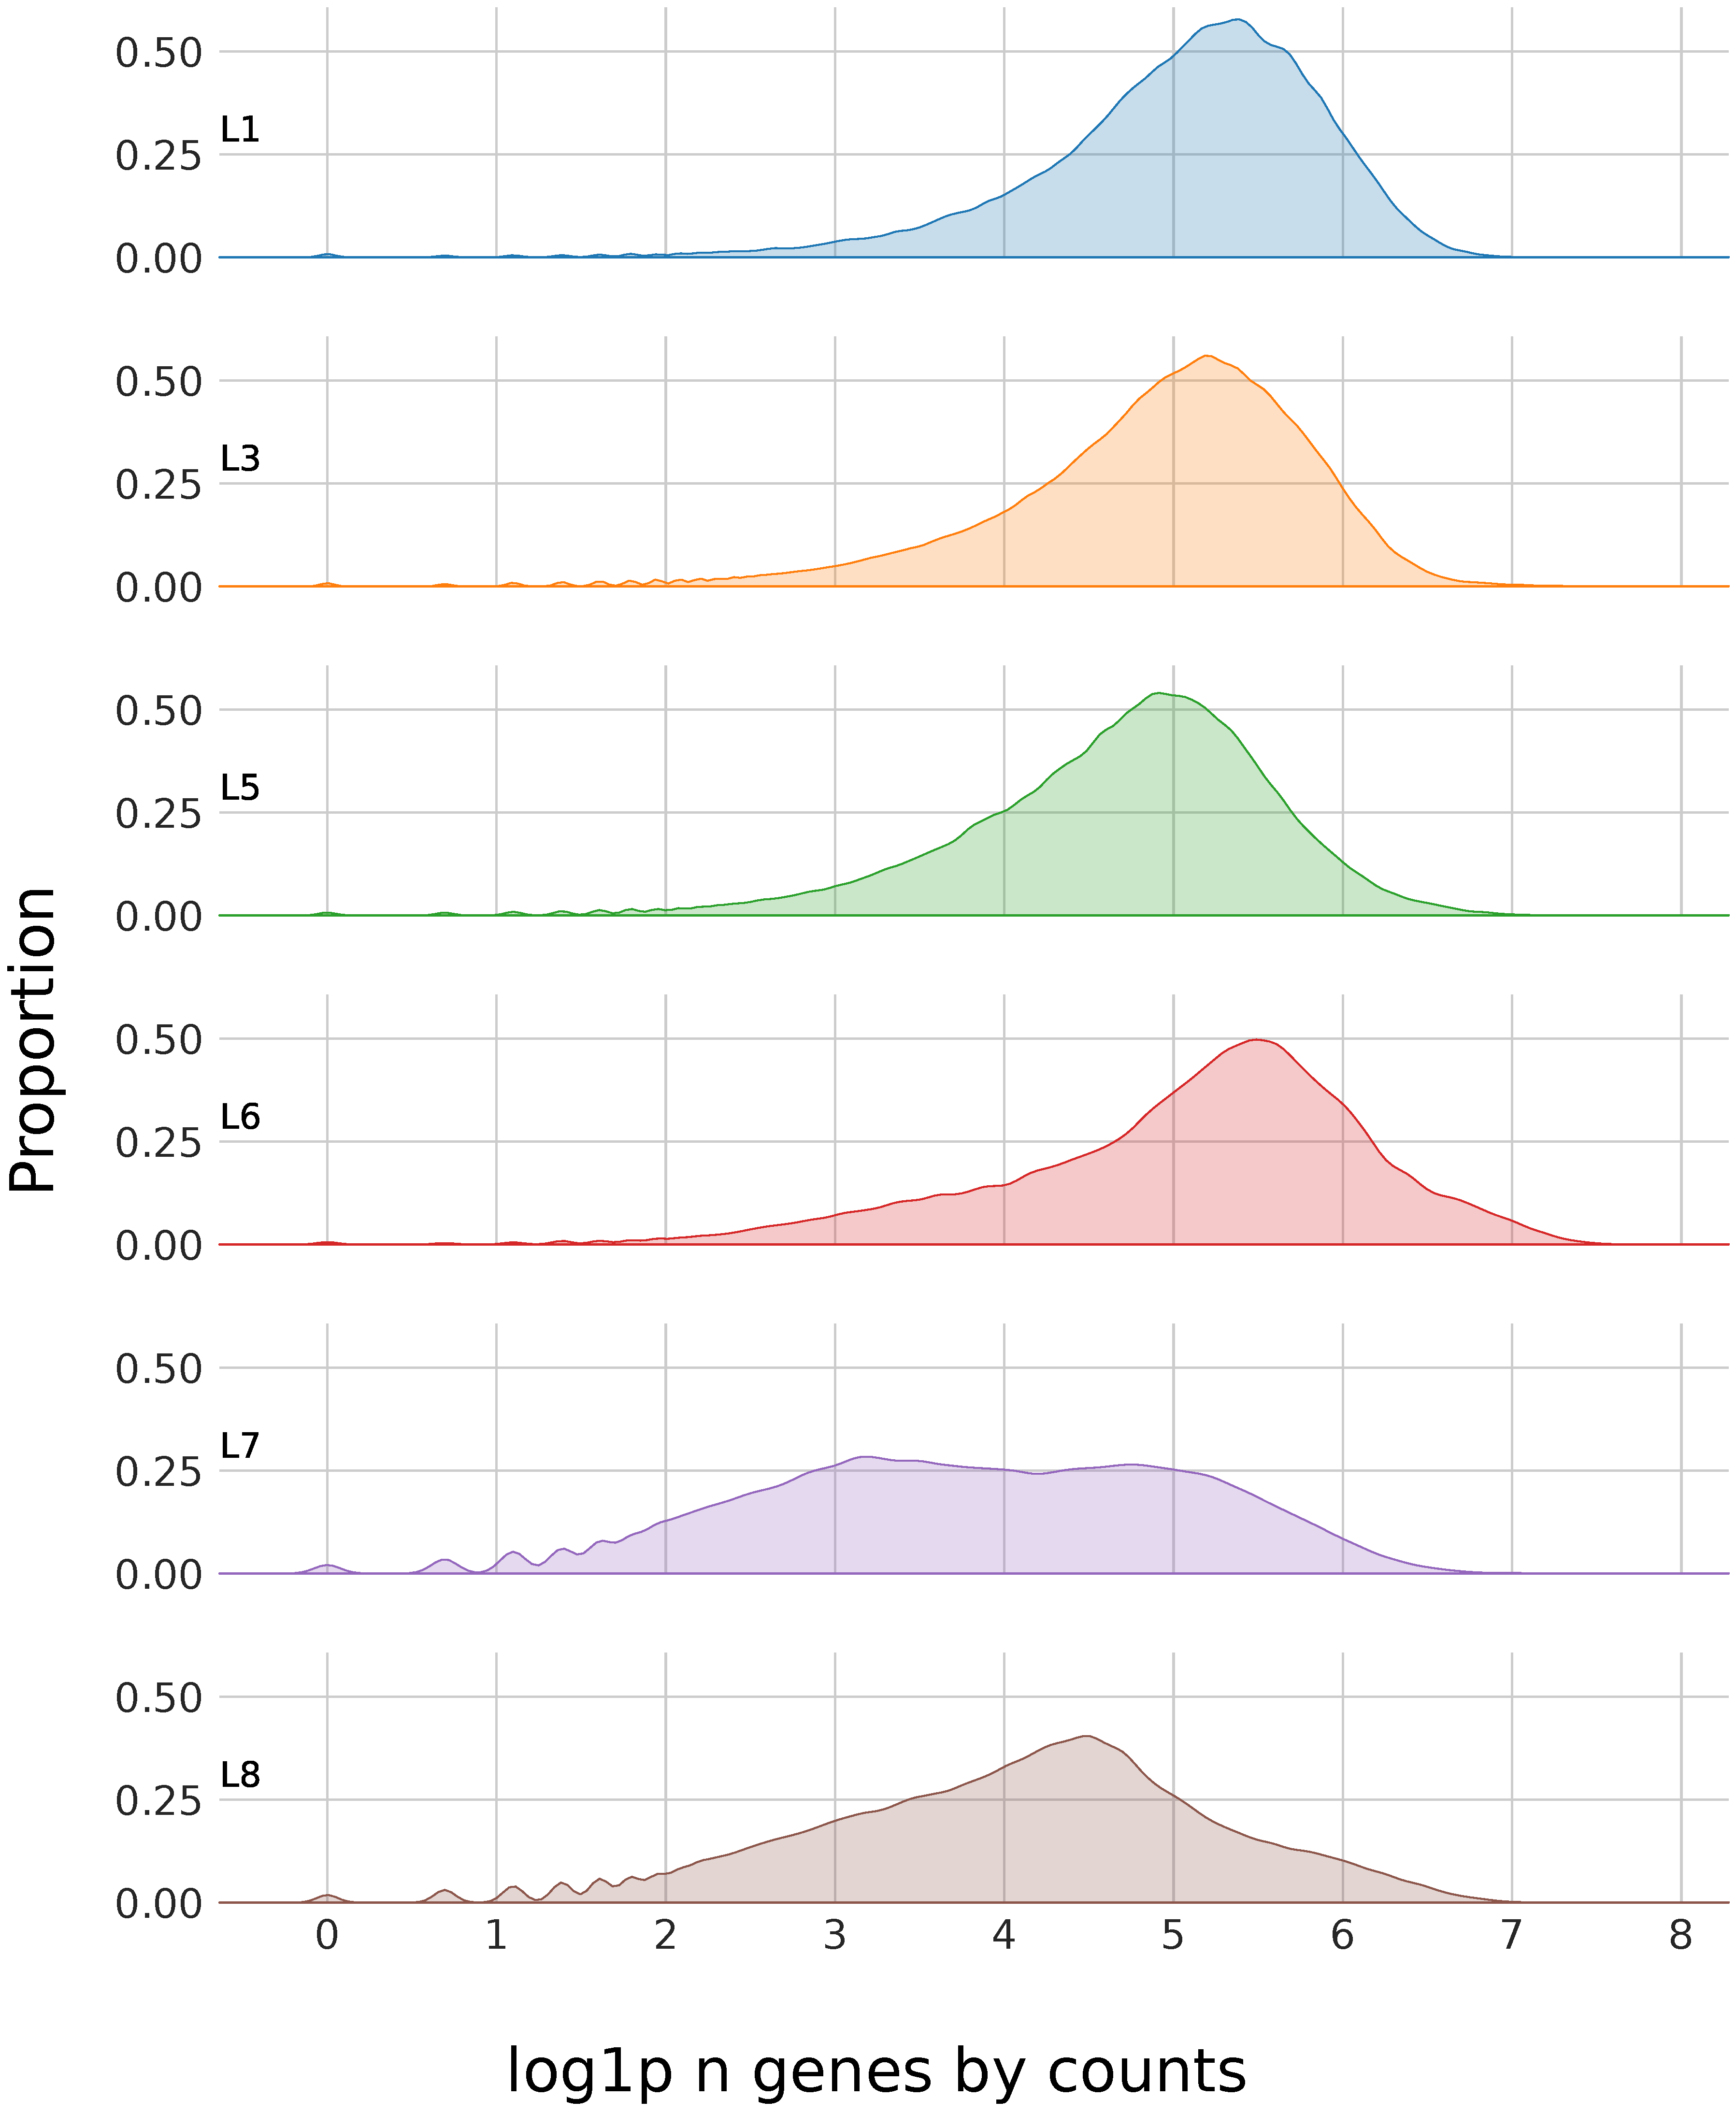
\includegraphics[width=\linewidth]{Figures/02_QC_expressed_genes/Cell-log1p_n_genes_by_counts-HistMutiple.pdf}
                        \caption{log1p(Genes by count)}
                    \end{figure}
                \end{column}
            \end{columns}
            \framebreak

            \begin{columns}
                \begin{column}{0.45 \textwidth}
                    \begin{figure}
                        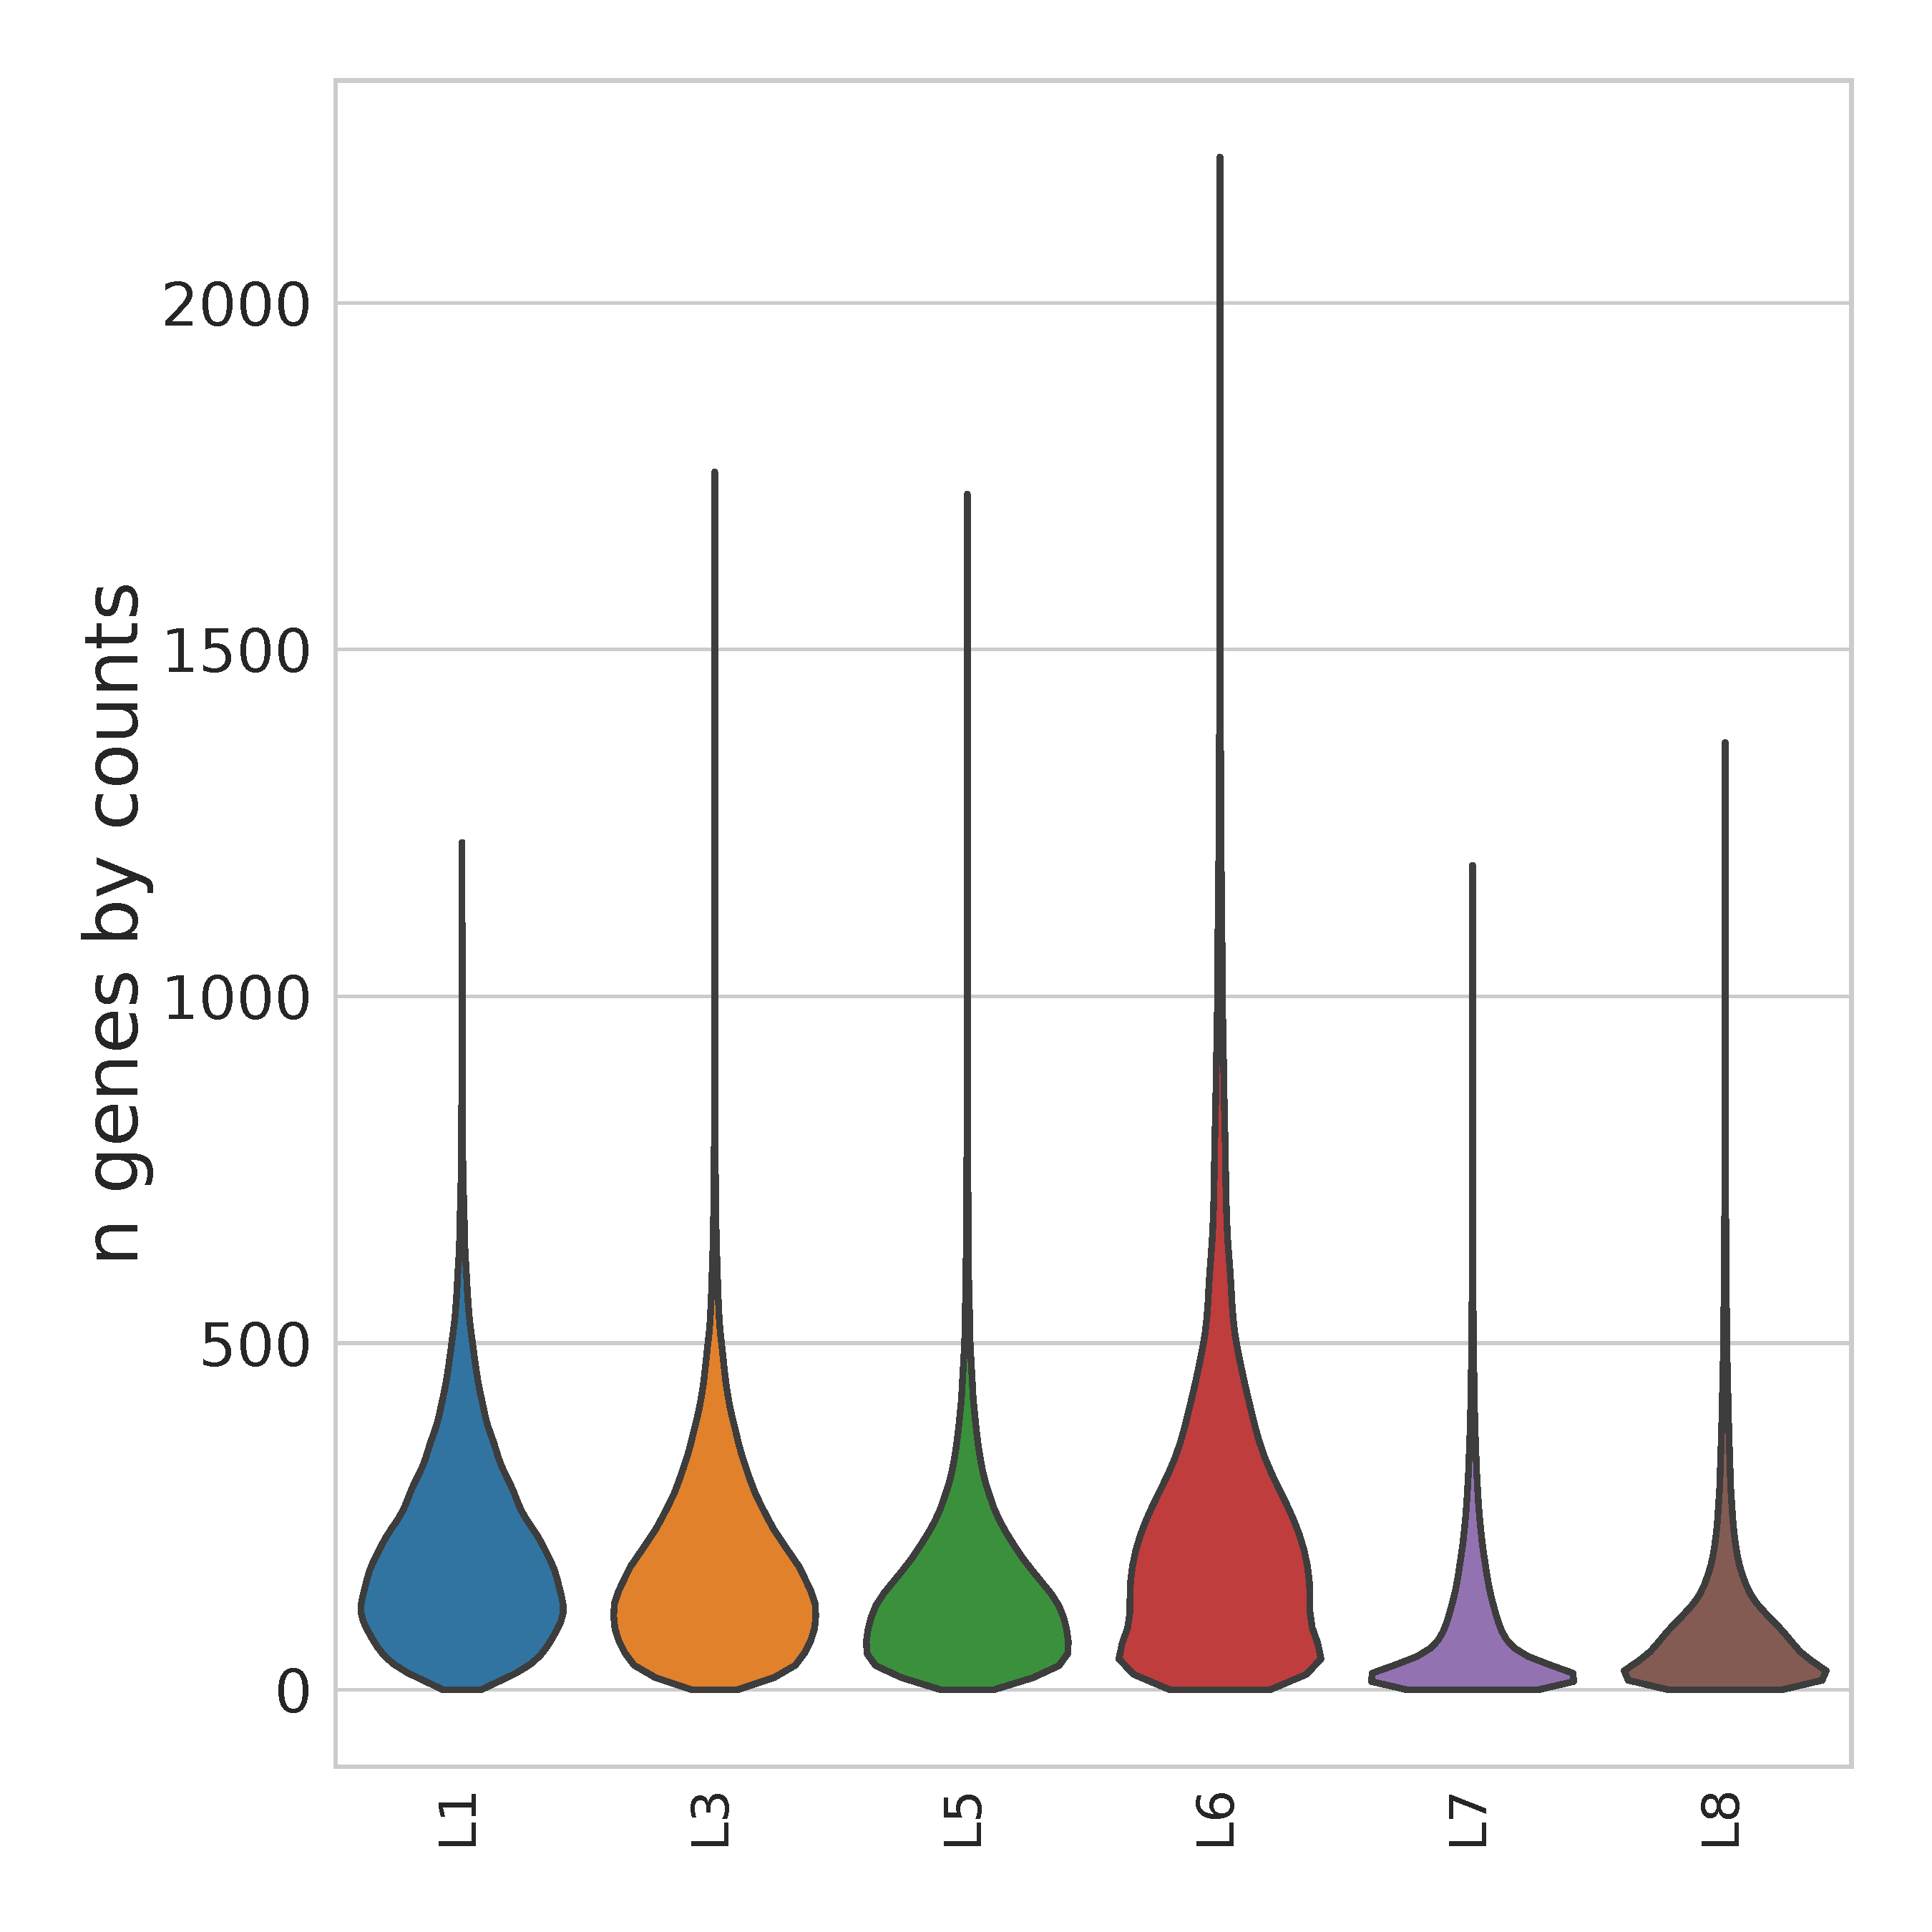
\includegraphics[width=\linewidth]{Figures/02_QC_expressed_genes/Cell-n_genes_by_counts-Violin.pdf}
                        \caption{Genes by counts}
                    \end{figure}
                \end{column}
                \begin{column}{0.45 \textwidth}
                    \begin{figure}
                        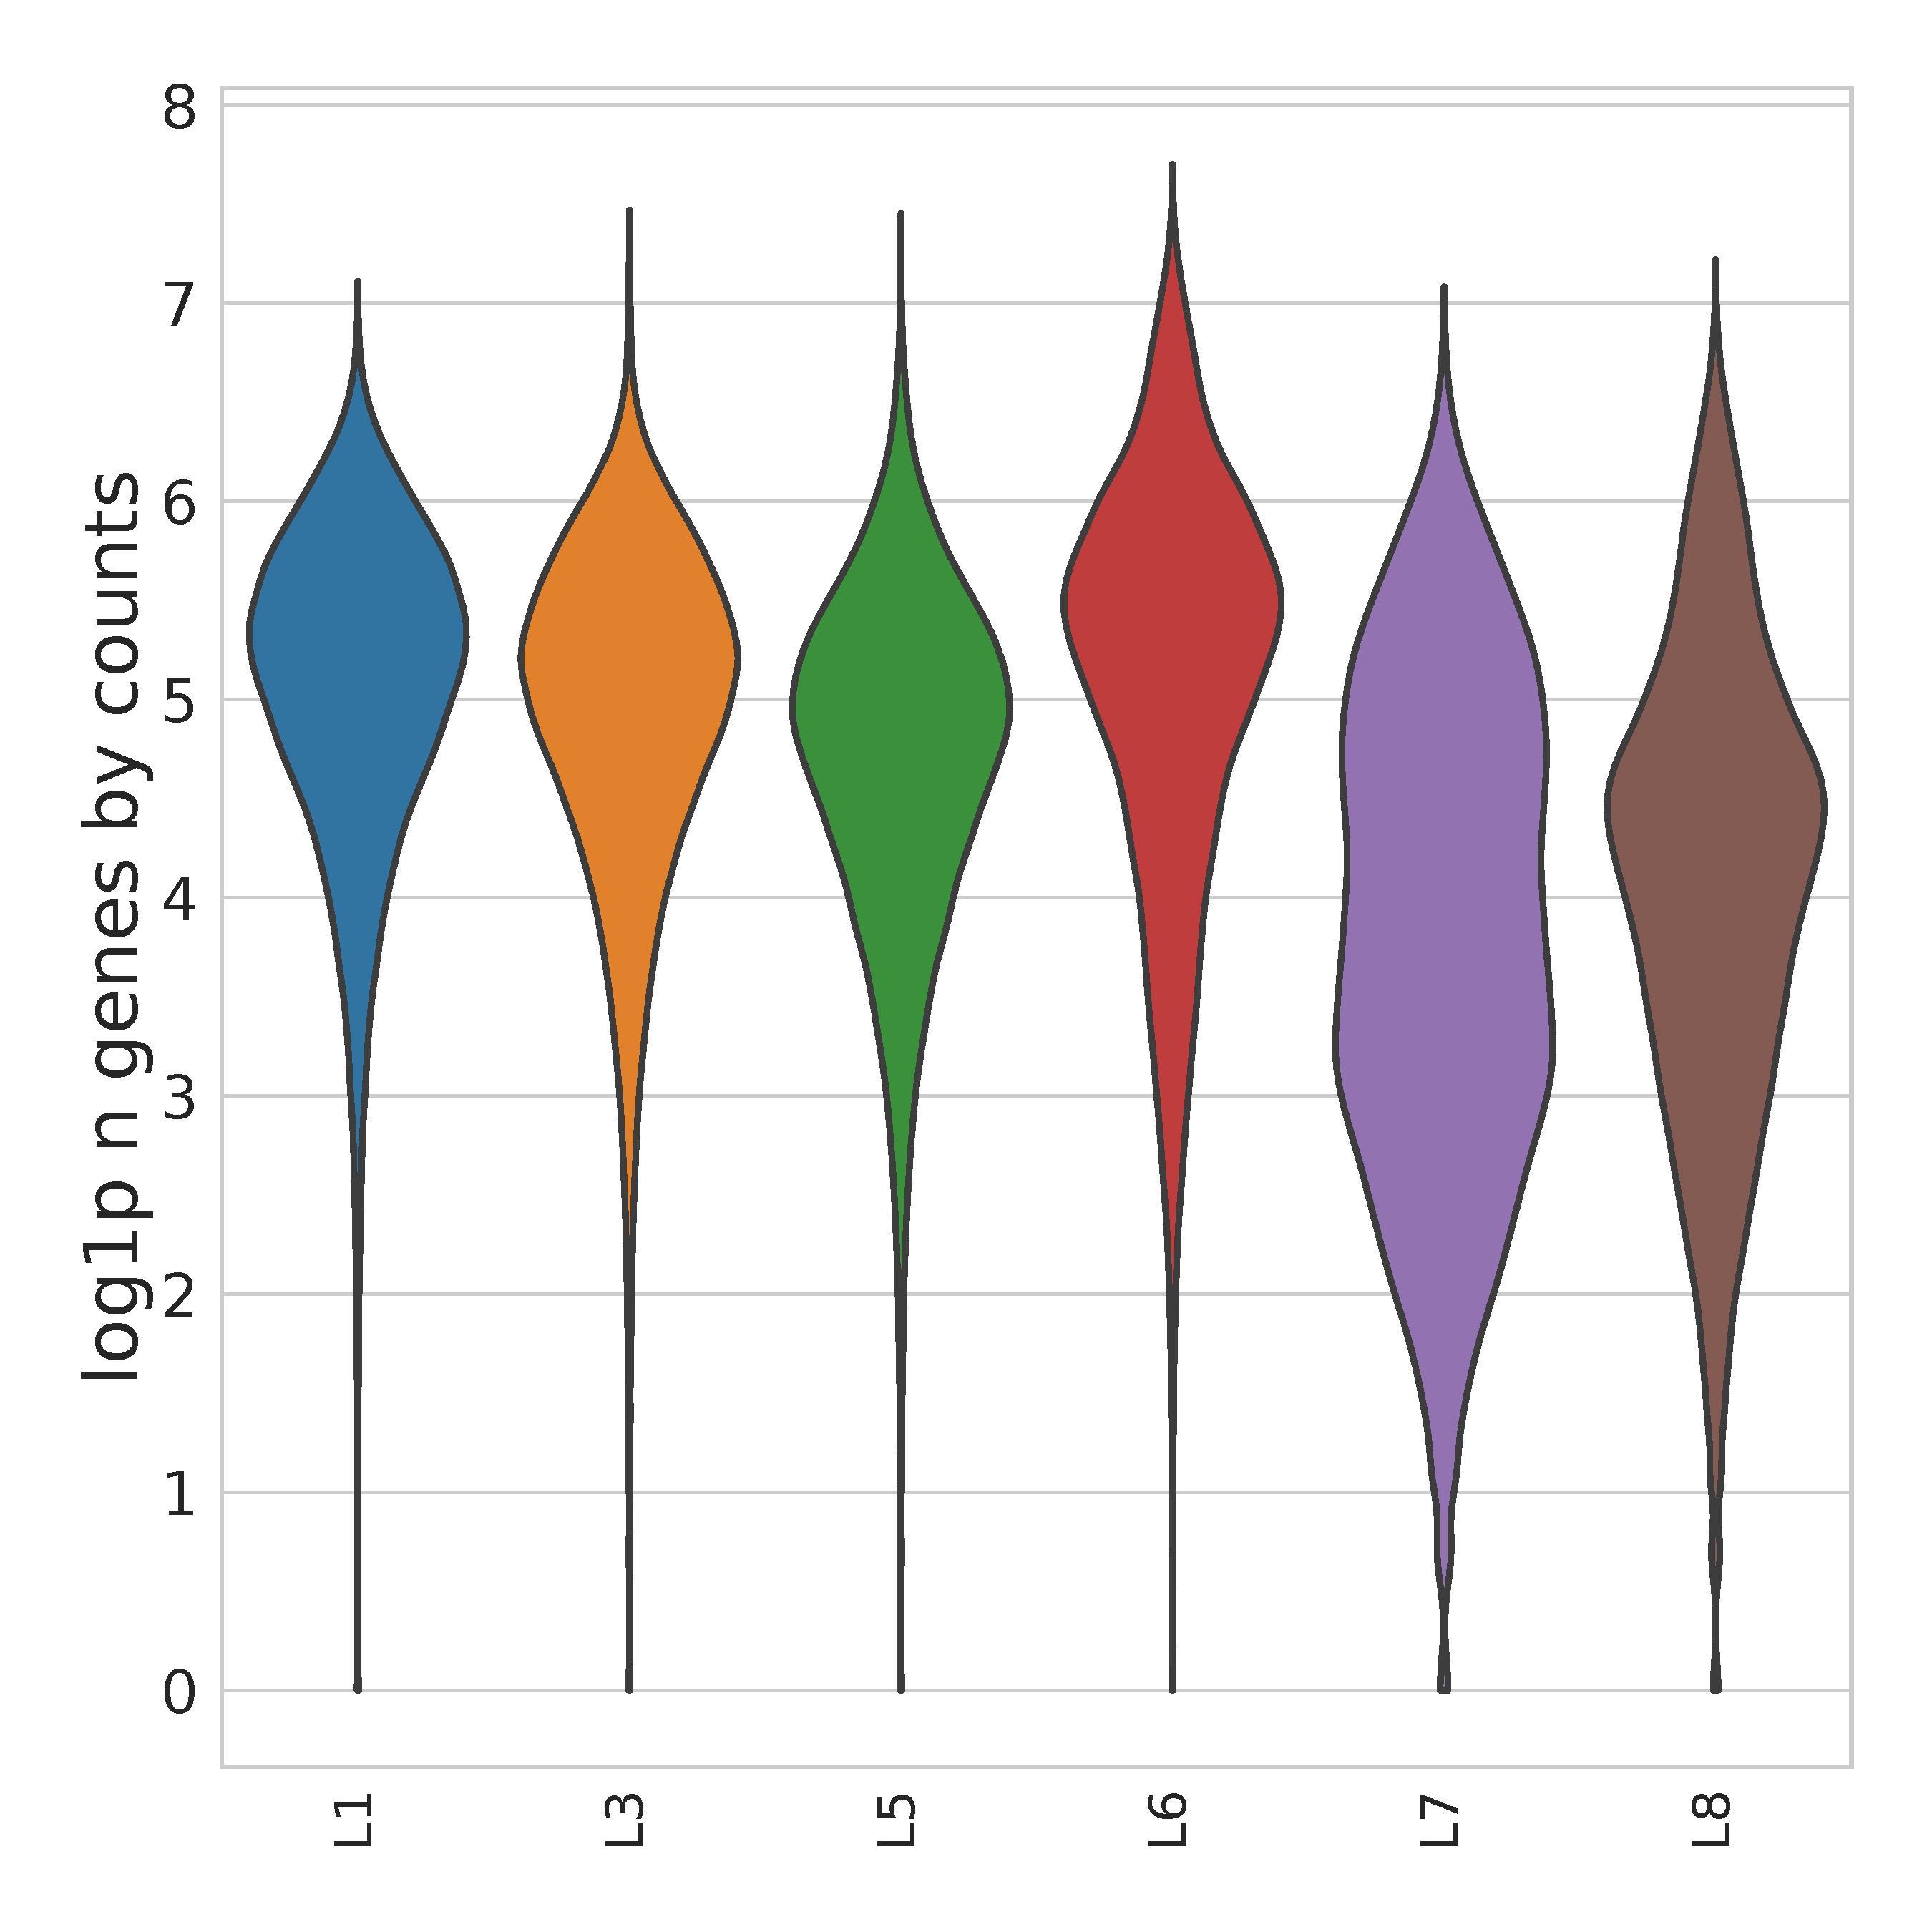
\includegraphics[width=\linewidth]{Figures/02_QC_expressed_genes/Cell-log1p_n_genes_by_counts-Violin.pdf}
                        \caption{log1p(Genes by count)}
                    \end{figure}
                \end{column}
            \end{columns}
            \framebreak
        \end{frame}

    \subsection{Highly variable genes}
    \begin{frame}[allowframebreaks]
        \frametitle{Highly variable genes with normalized dispersions}

        \begin{columns}
            \begin{column}{0.45 \textwidth}
                \begin{figure}
                    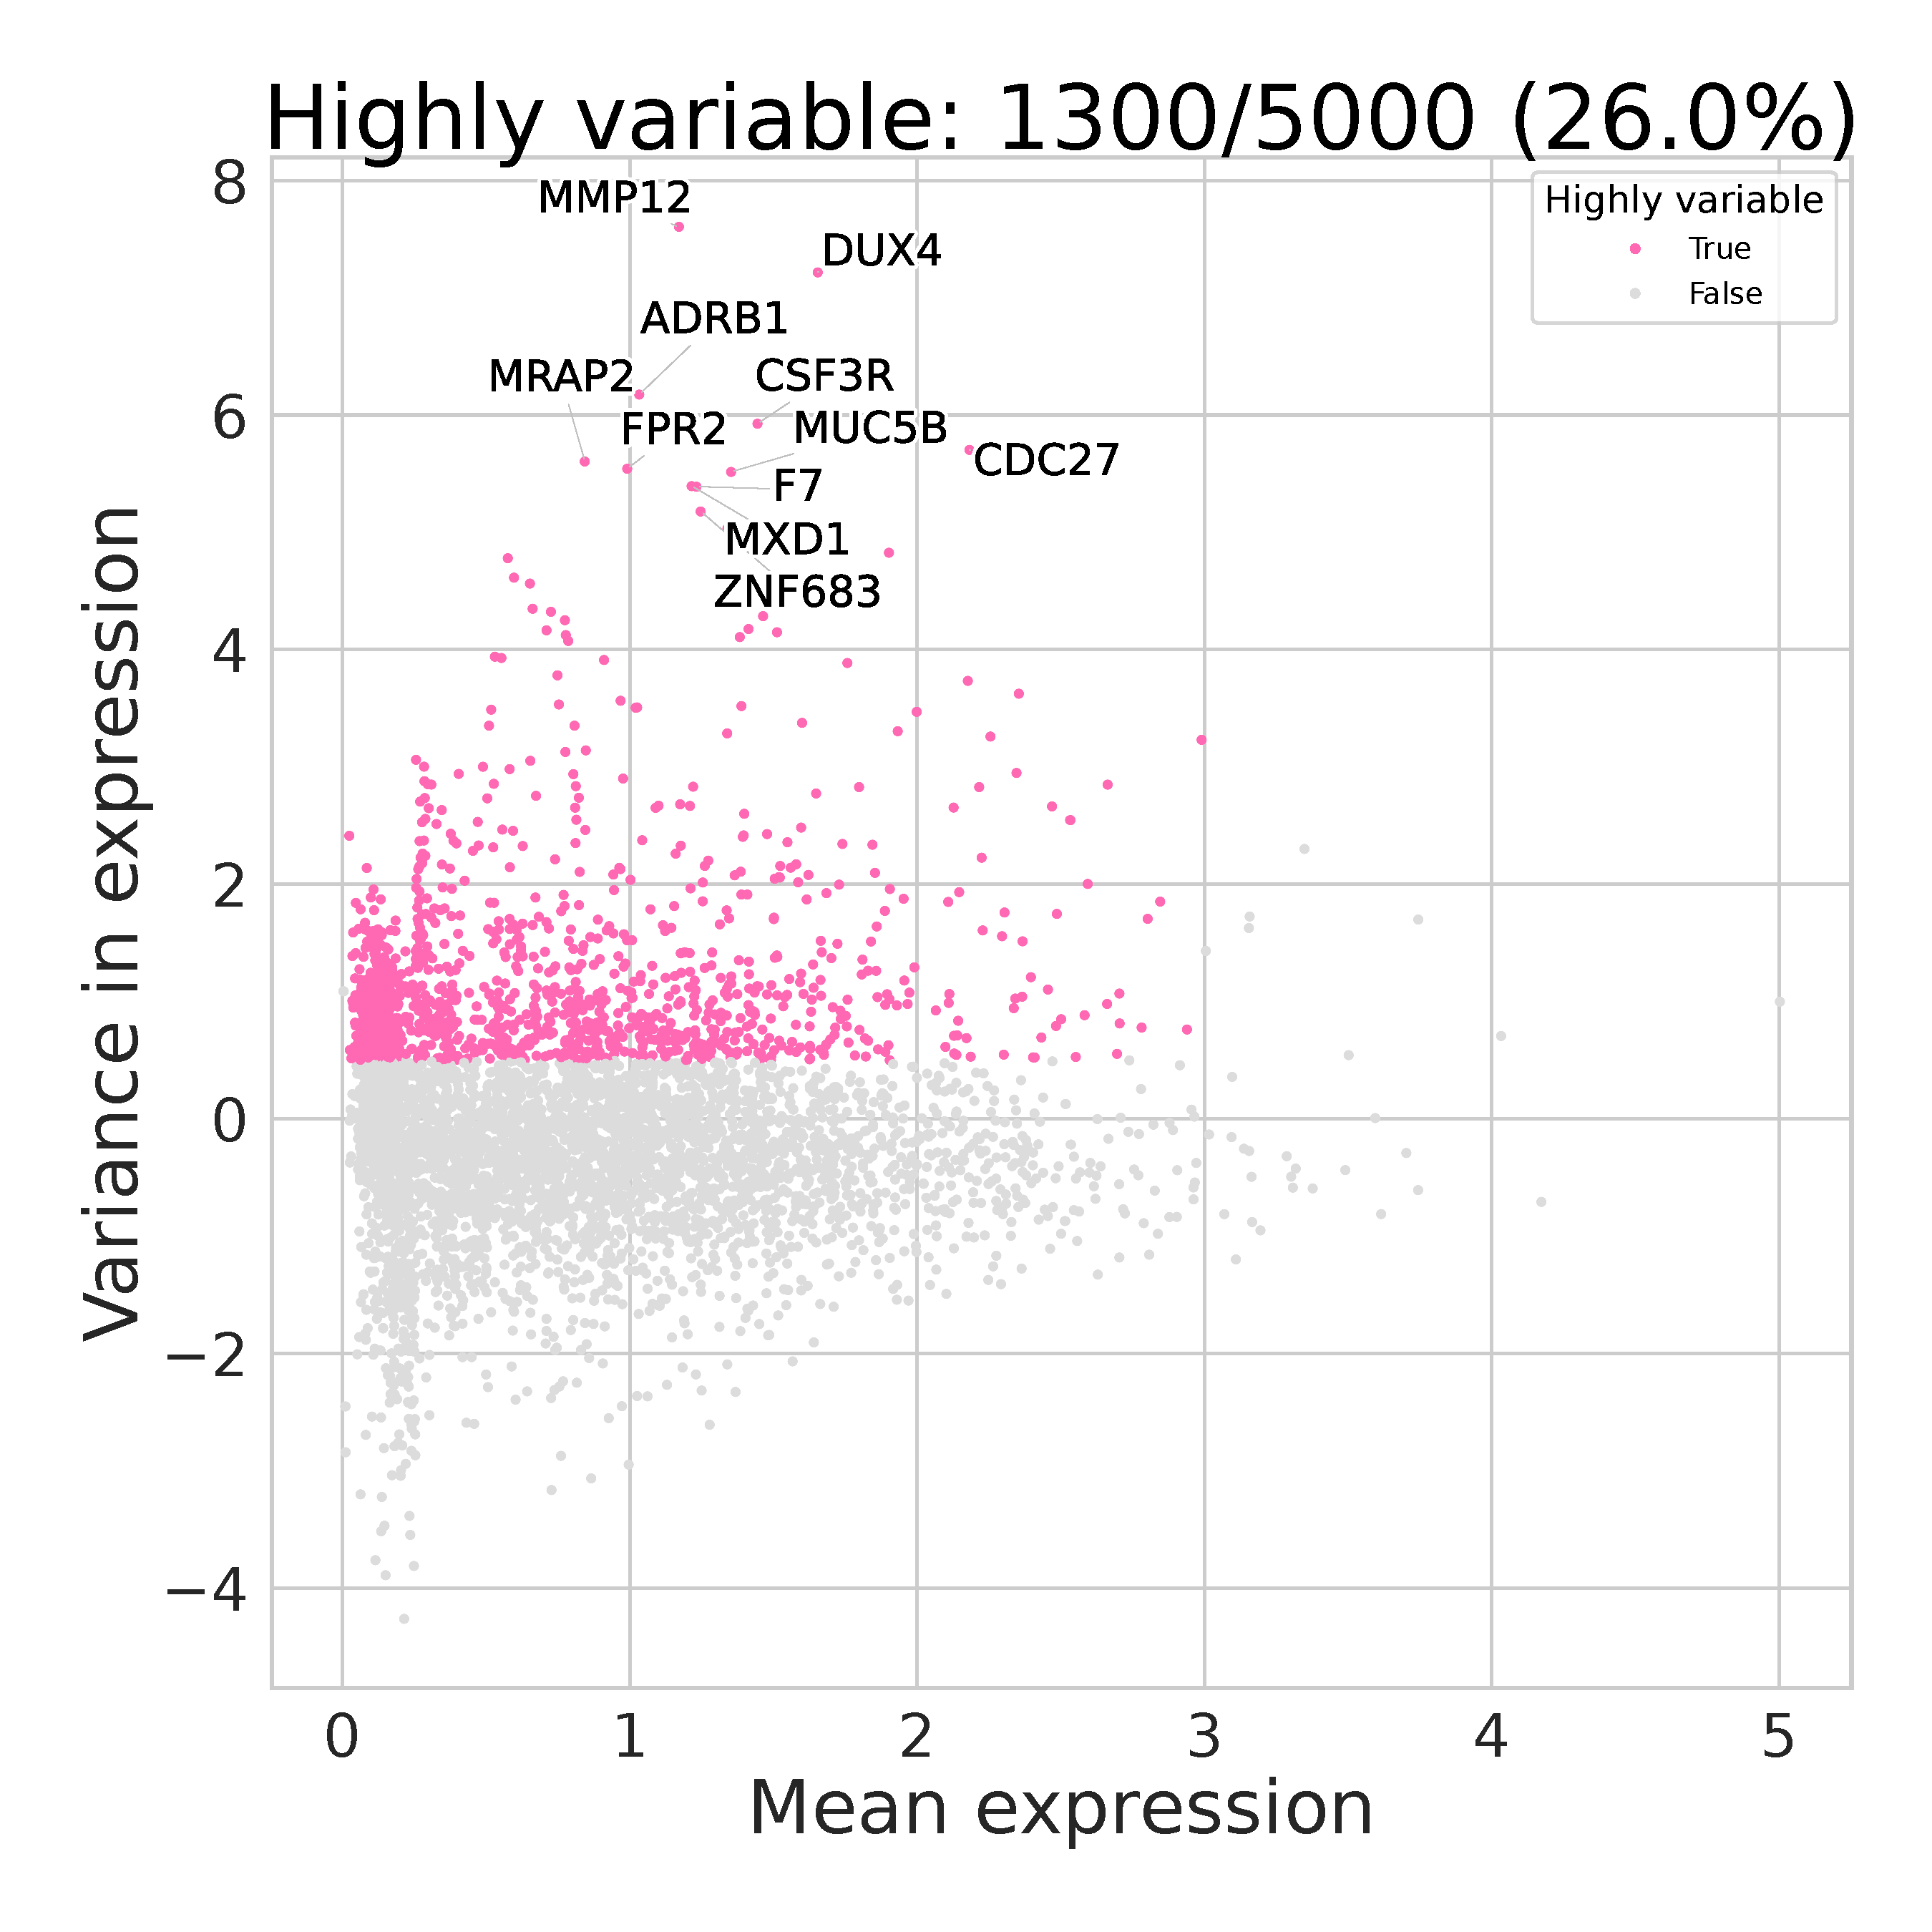
\includegraphics[width=\linewidth]{Figures/04_Highly_variable_genes/Scatter-dispersions_norm.pdf}
                    \caption{Volcano plot}
                \end{figure}
            \end{column}
            \begin{column}{0.45 \textwidth}
                \begin{figure}
                    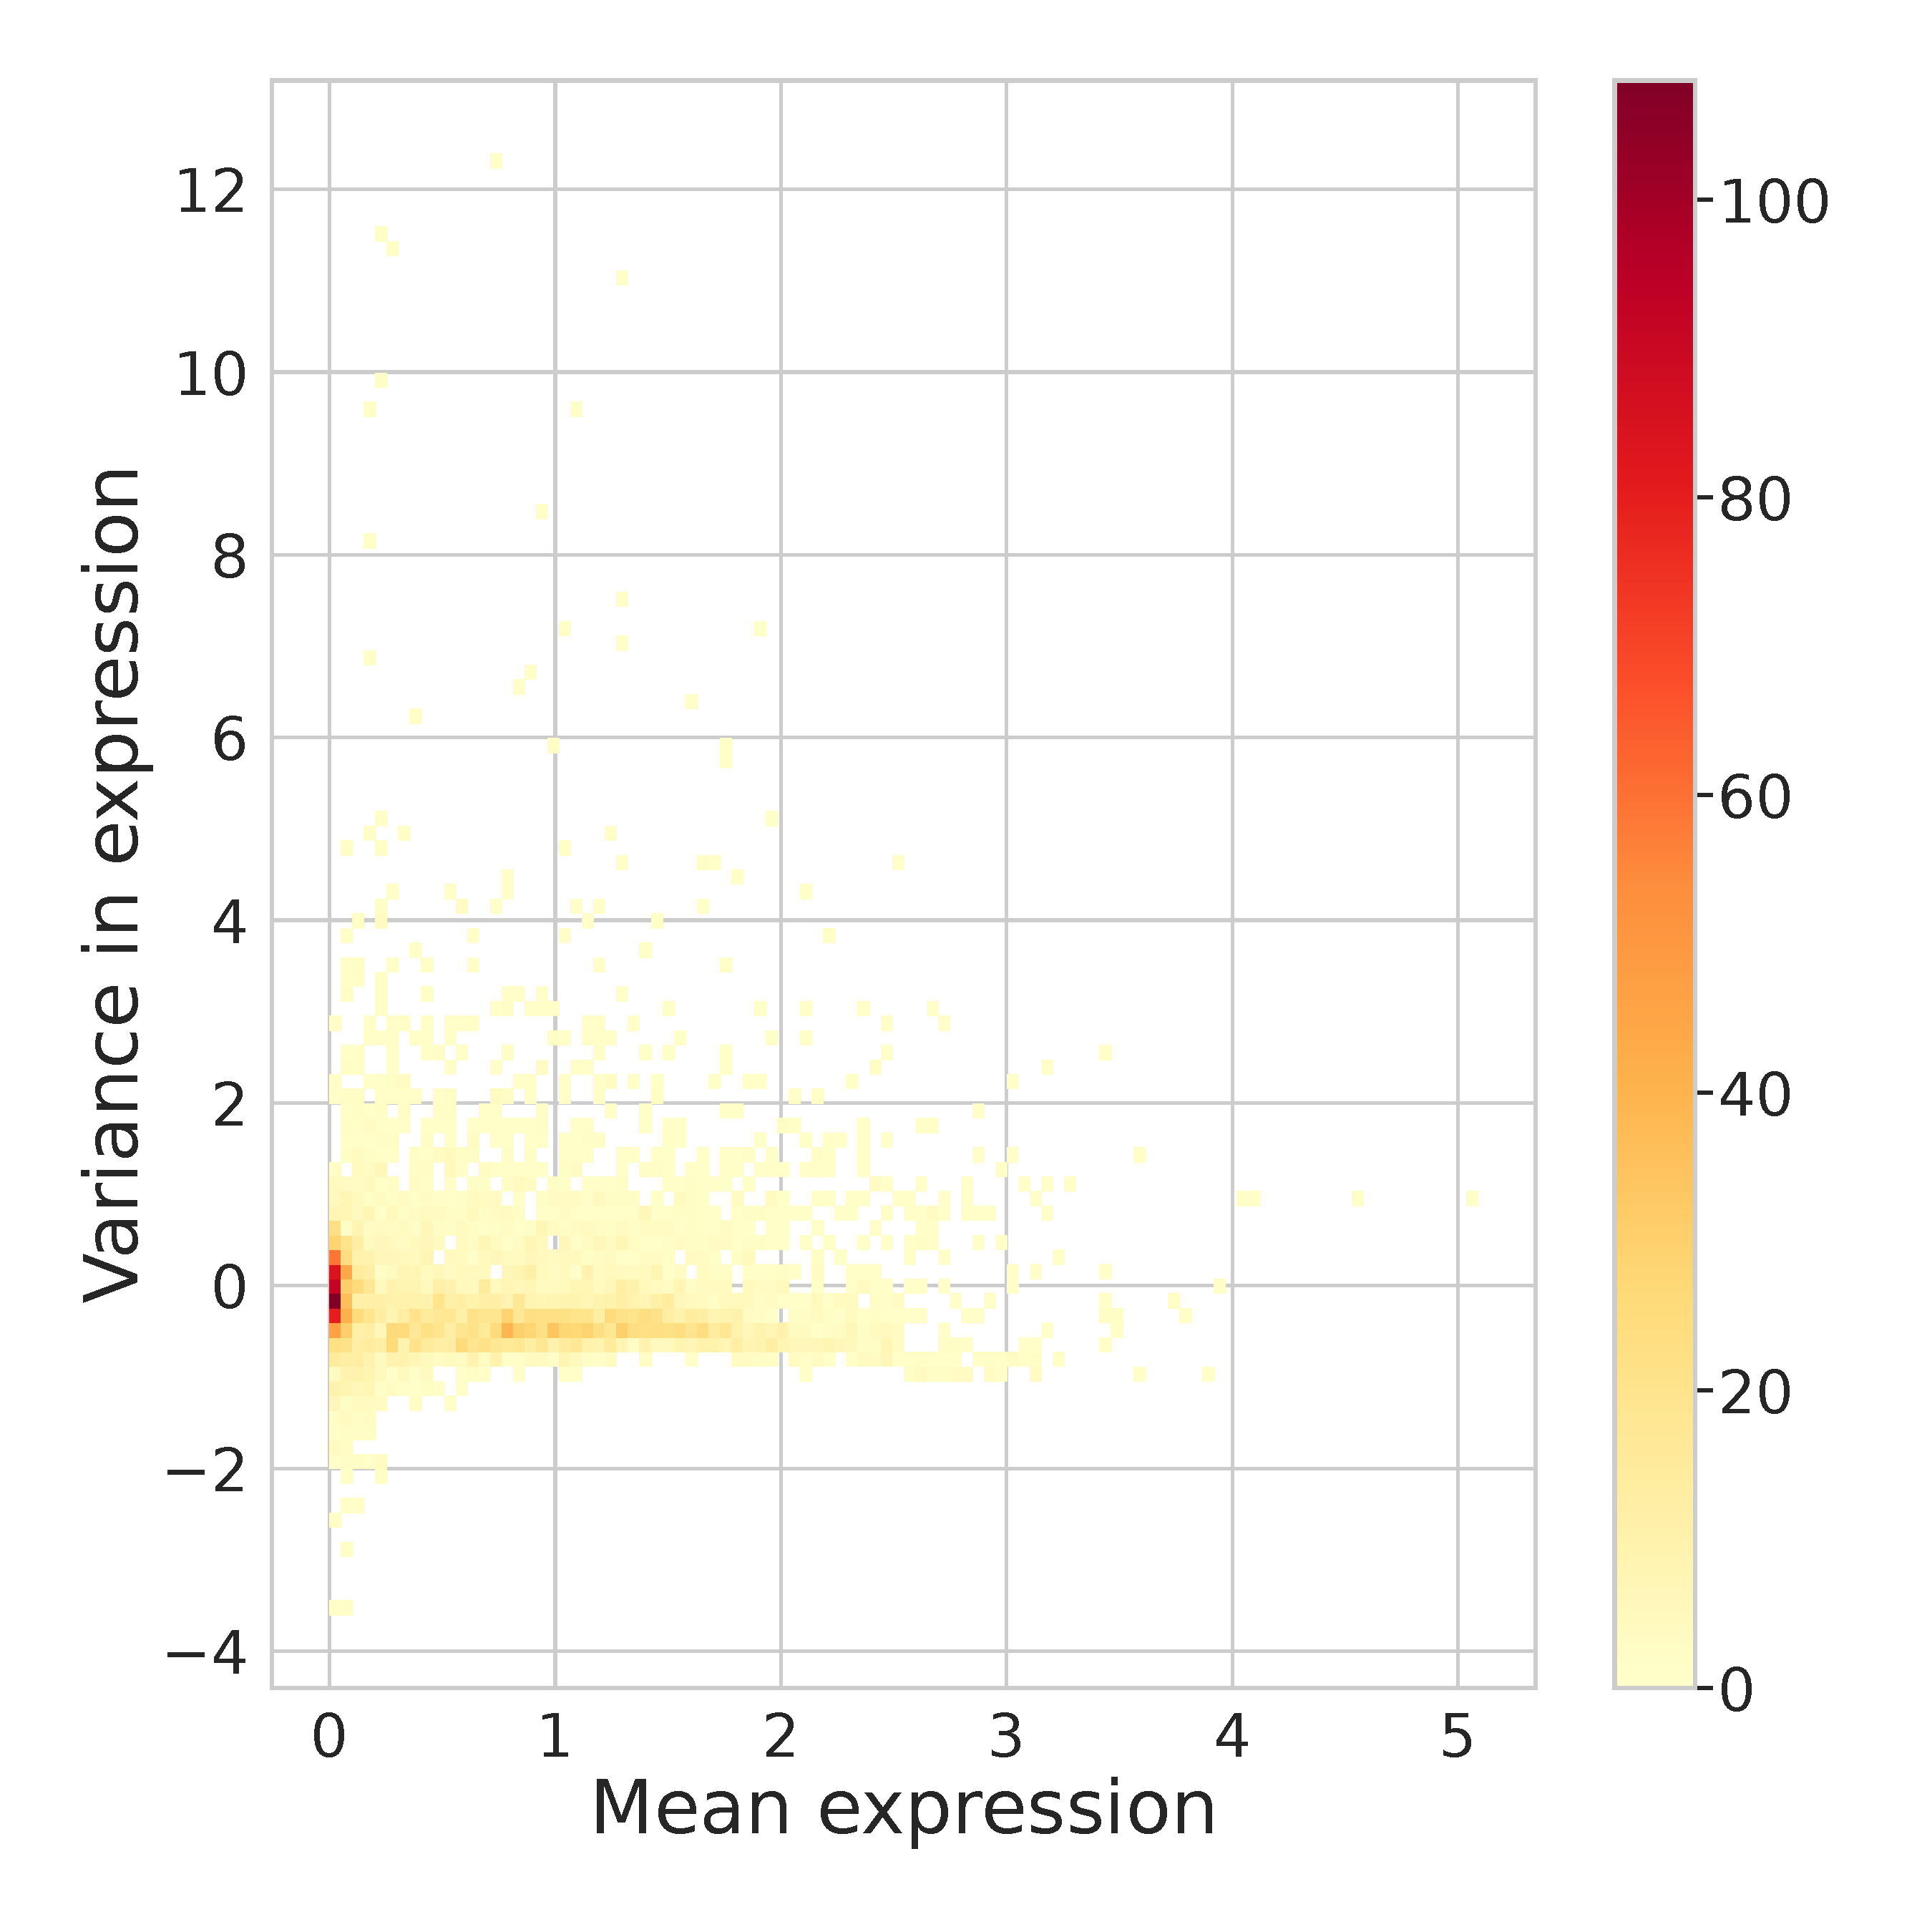
\includegraphics[width=\linewidth]{Figures/04_Highly_variable_genes/2DHist-dispersions_norm.pdf}
                    \caption{Distribution}
                \end{figure}
            \end{column}
        \end{columns}
        \framebreak

        \begin{figure}
            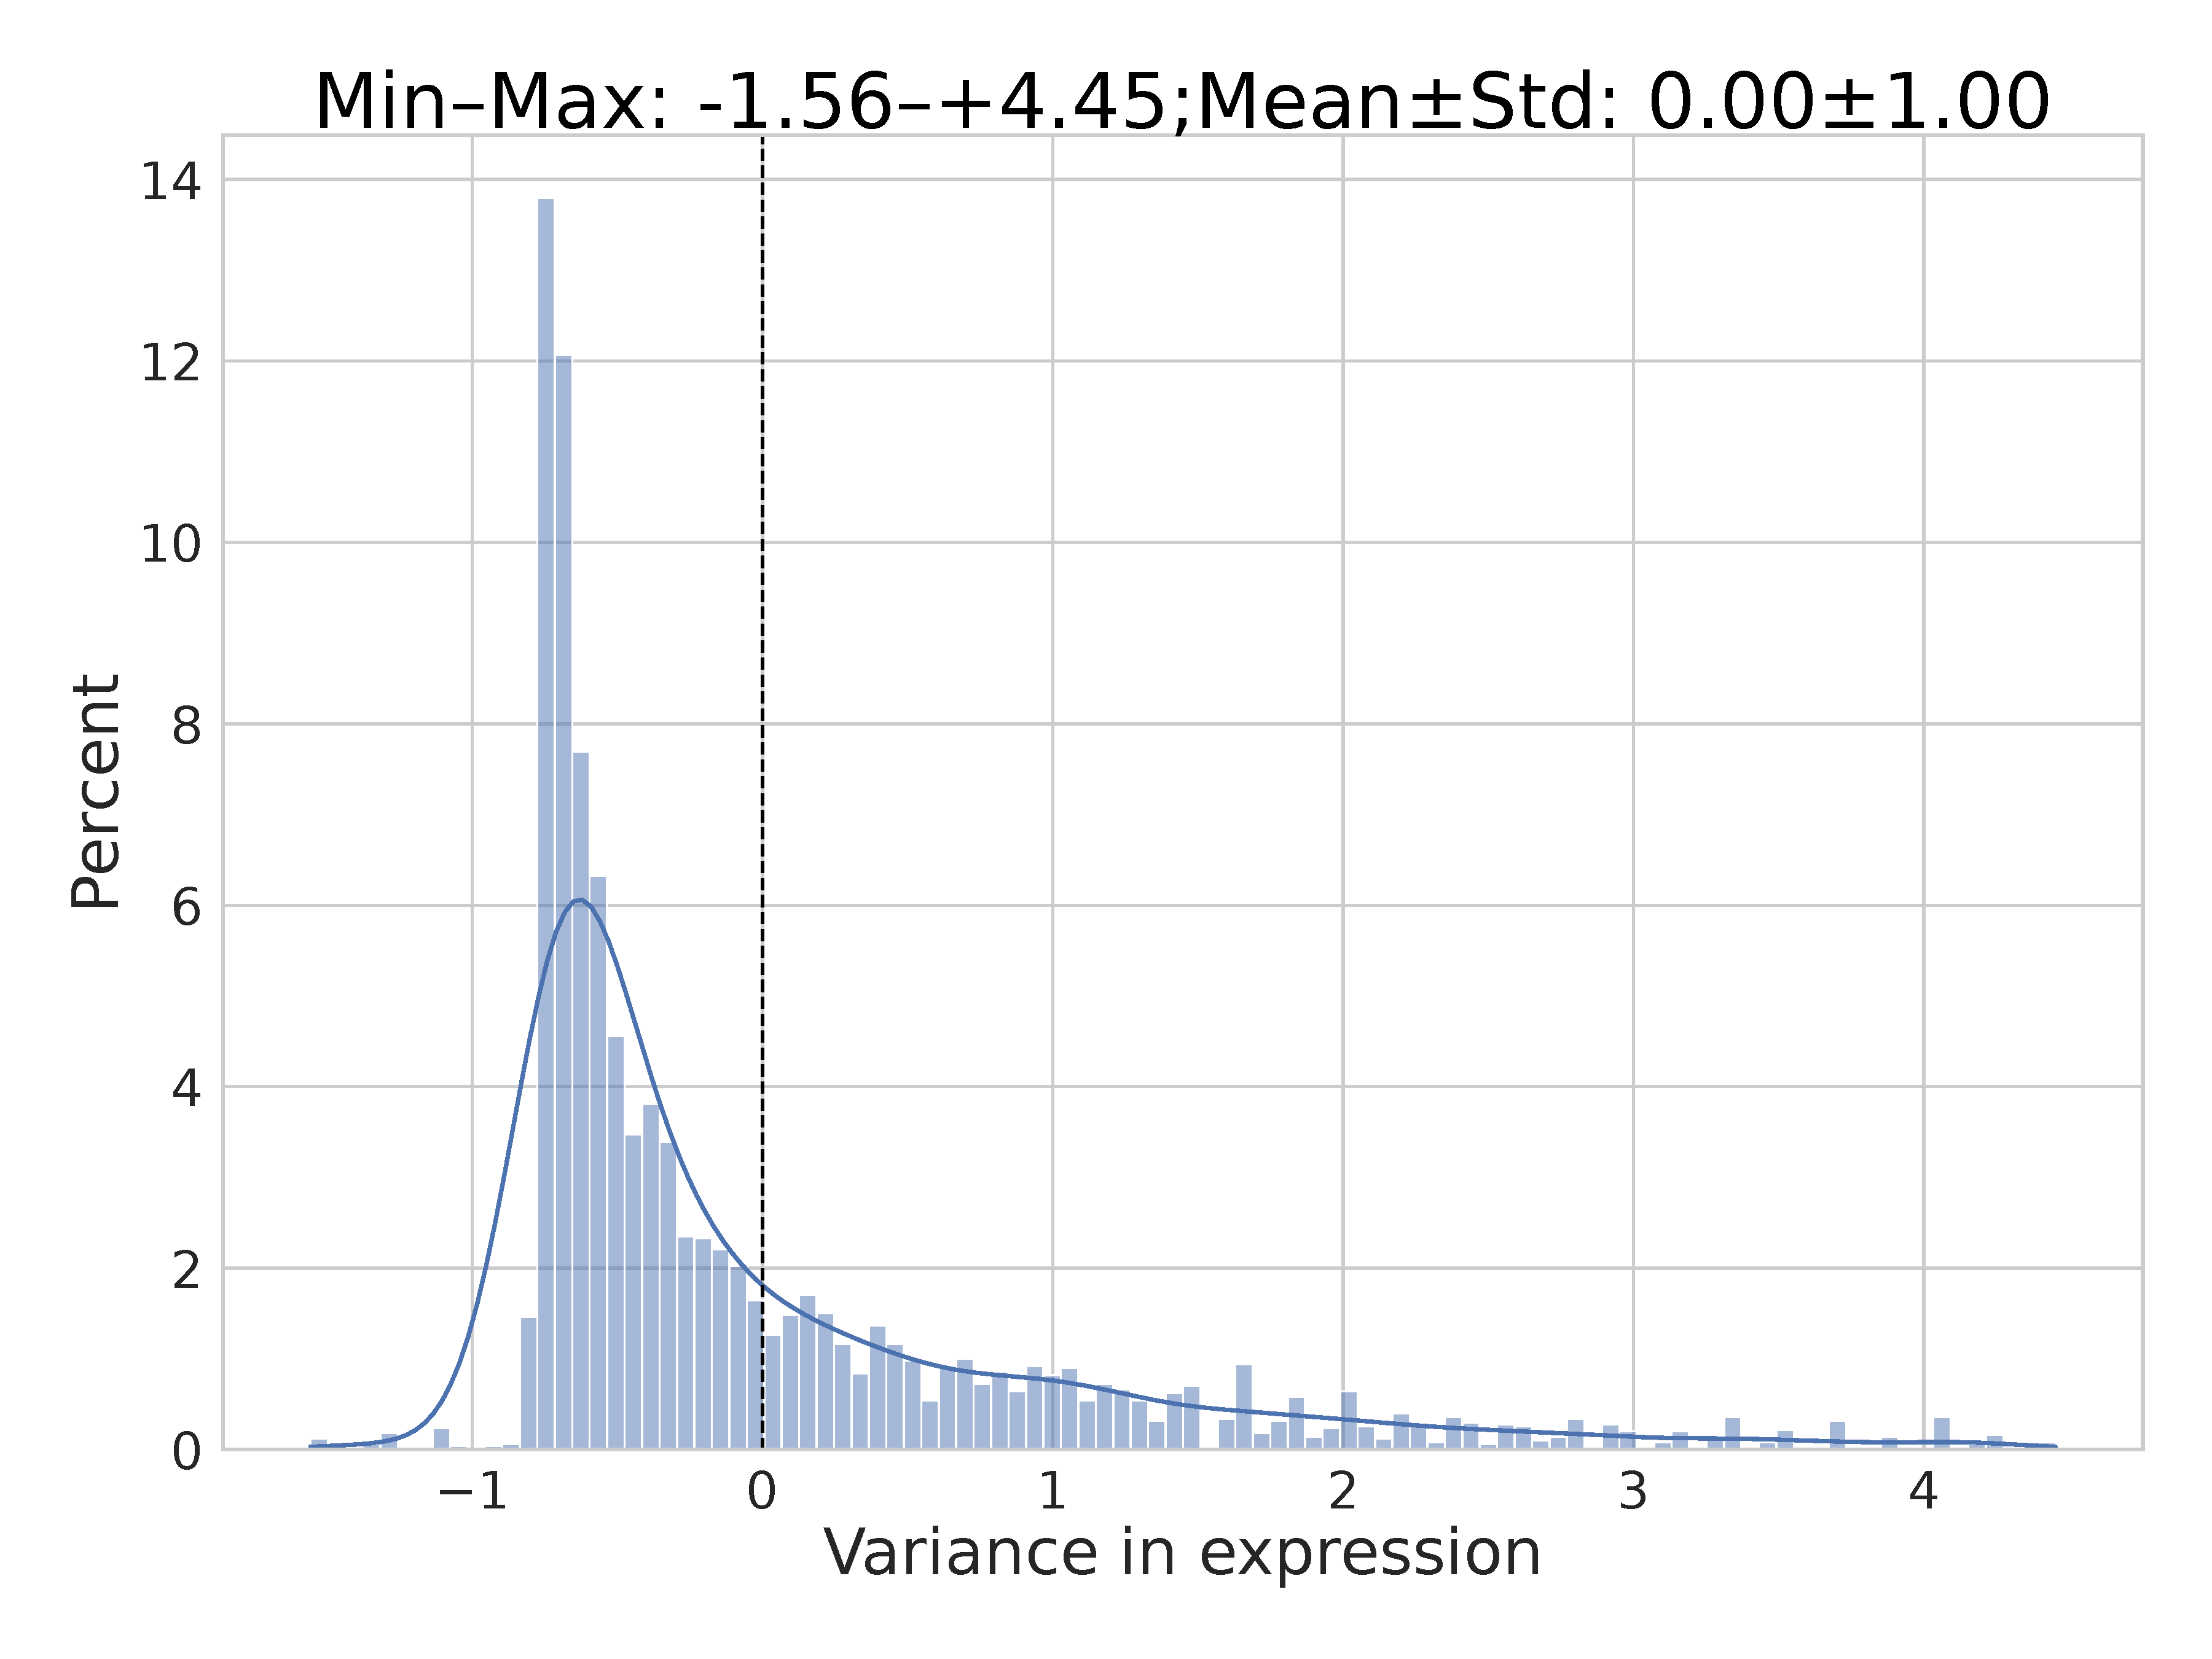
\includegraphics[width=0.6 \linewidth]{Figures/04_Highly_variable_genes/Distribution-dispersions_norm.pdf}
            \caption{Histogram}
        \end{figure}
    \end{frame}

    \begin{frame}[allowframebreaks]
        \frametitle{Highly variable genes with dispersions}

        \begin{columns}
            \begin{column}{0.45 \textwidth}
                \begin{figure}
                    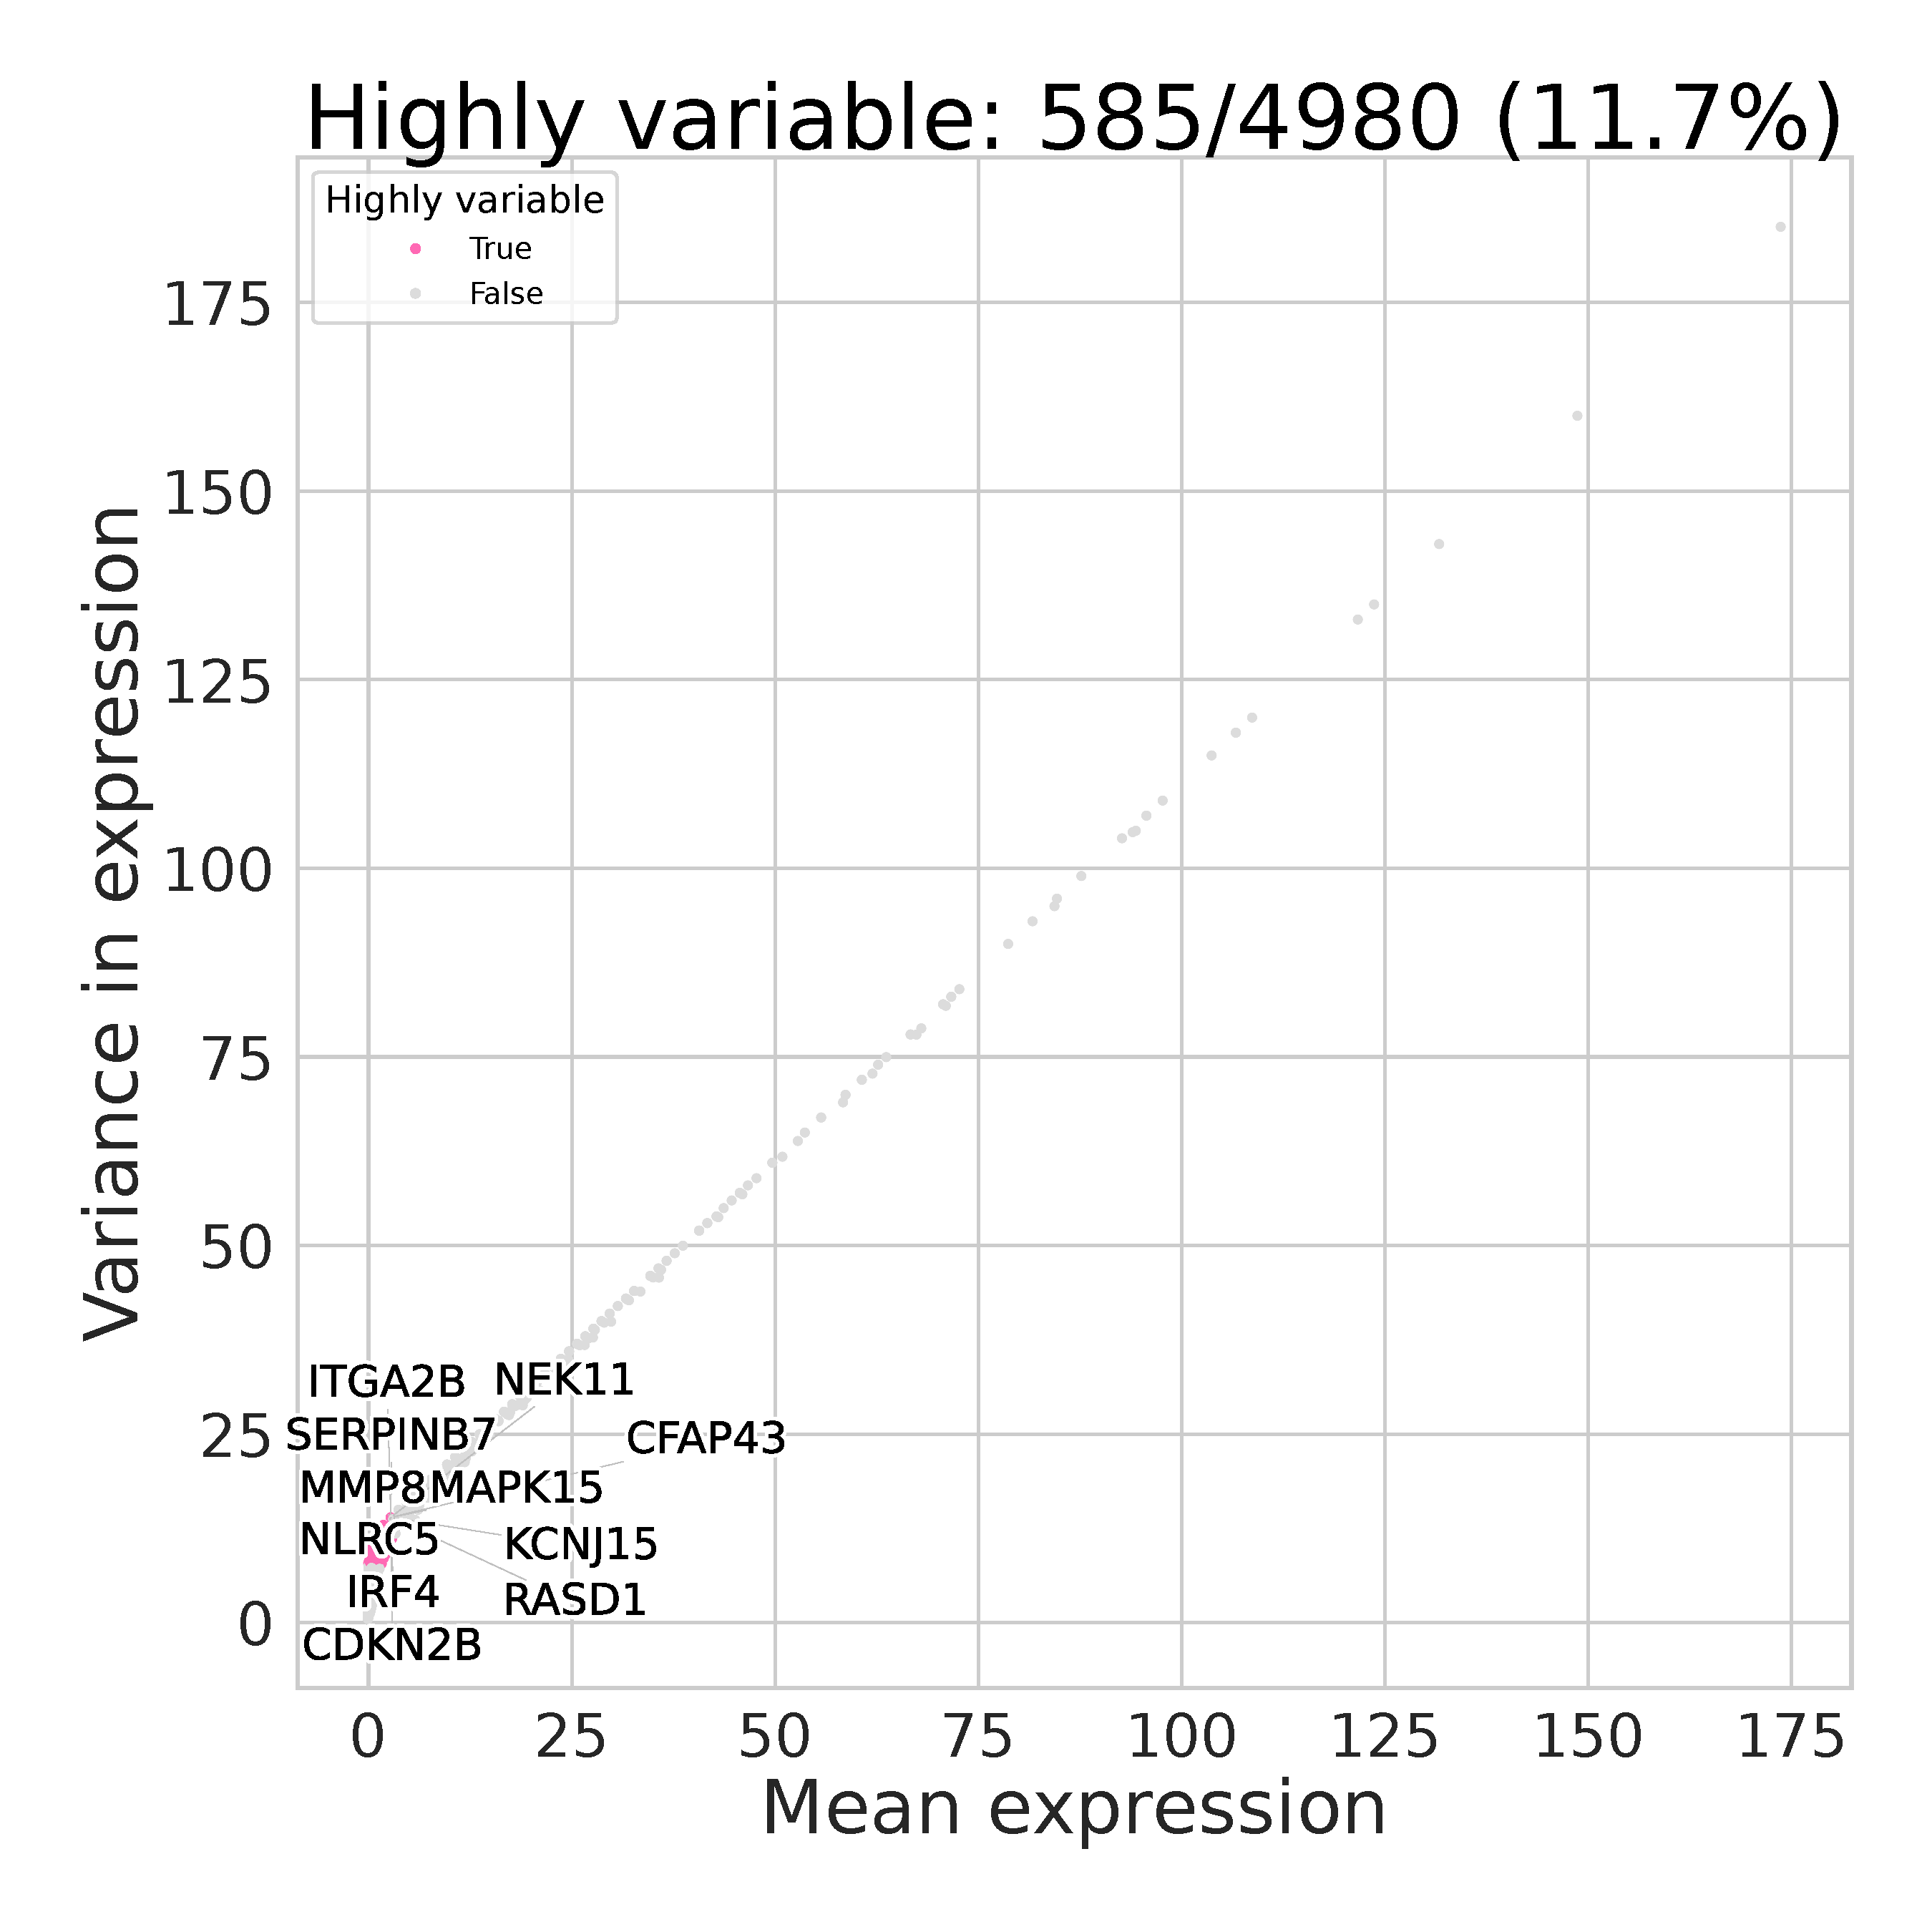
\includegraphics[width=\linewidth]{Figures/04_Highly_variable_genes/Scatter-dispersions.pdf}
                    \caption{Volcano plot}
                \end{figure}
            \end{column}
            \begin{column}{0.45 \textwidth}
                \begin{figure}
                    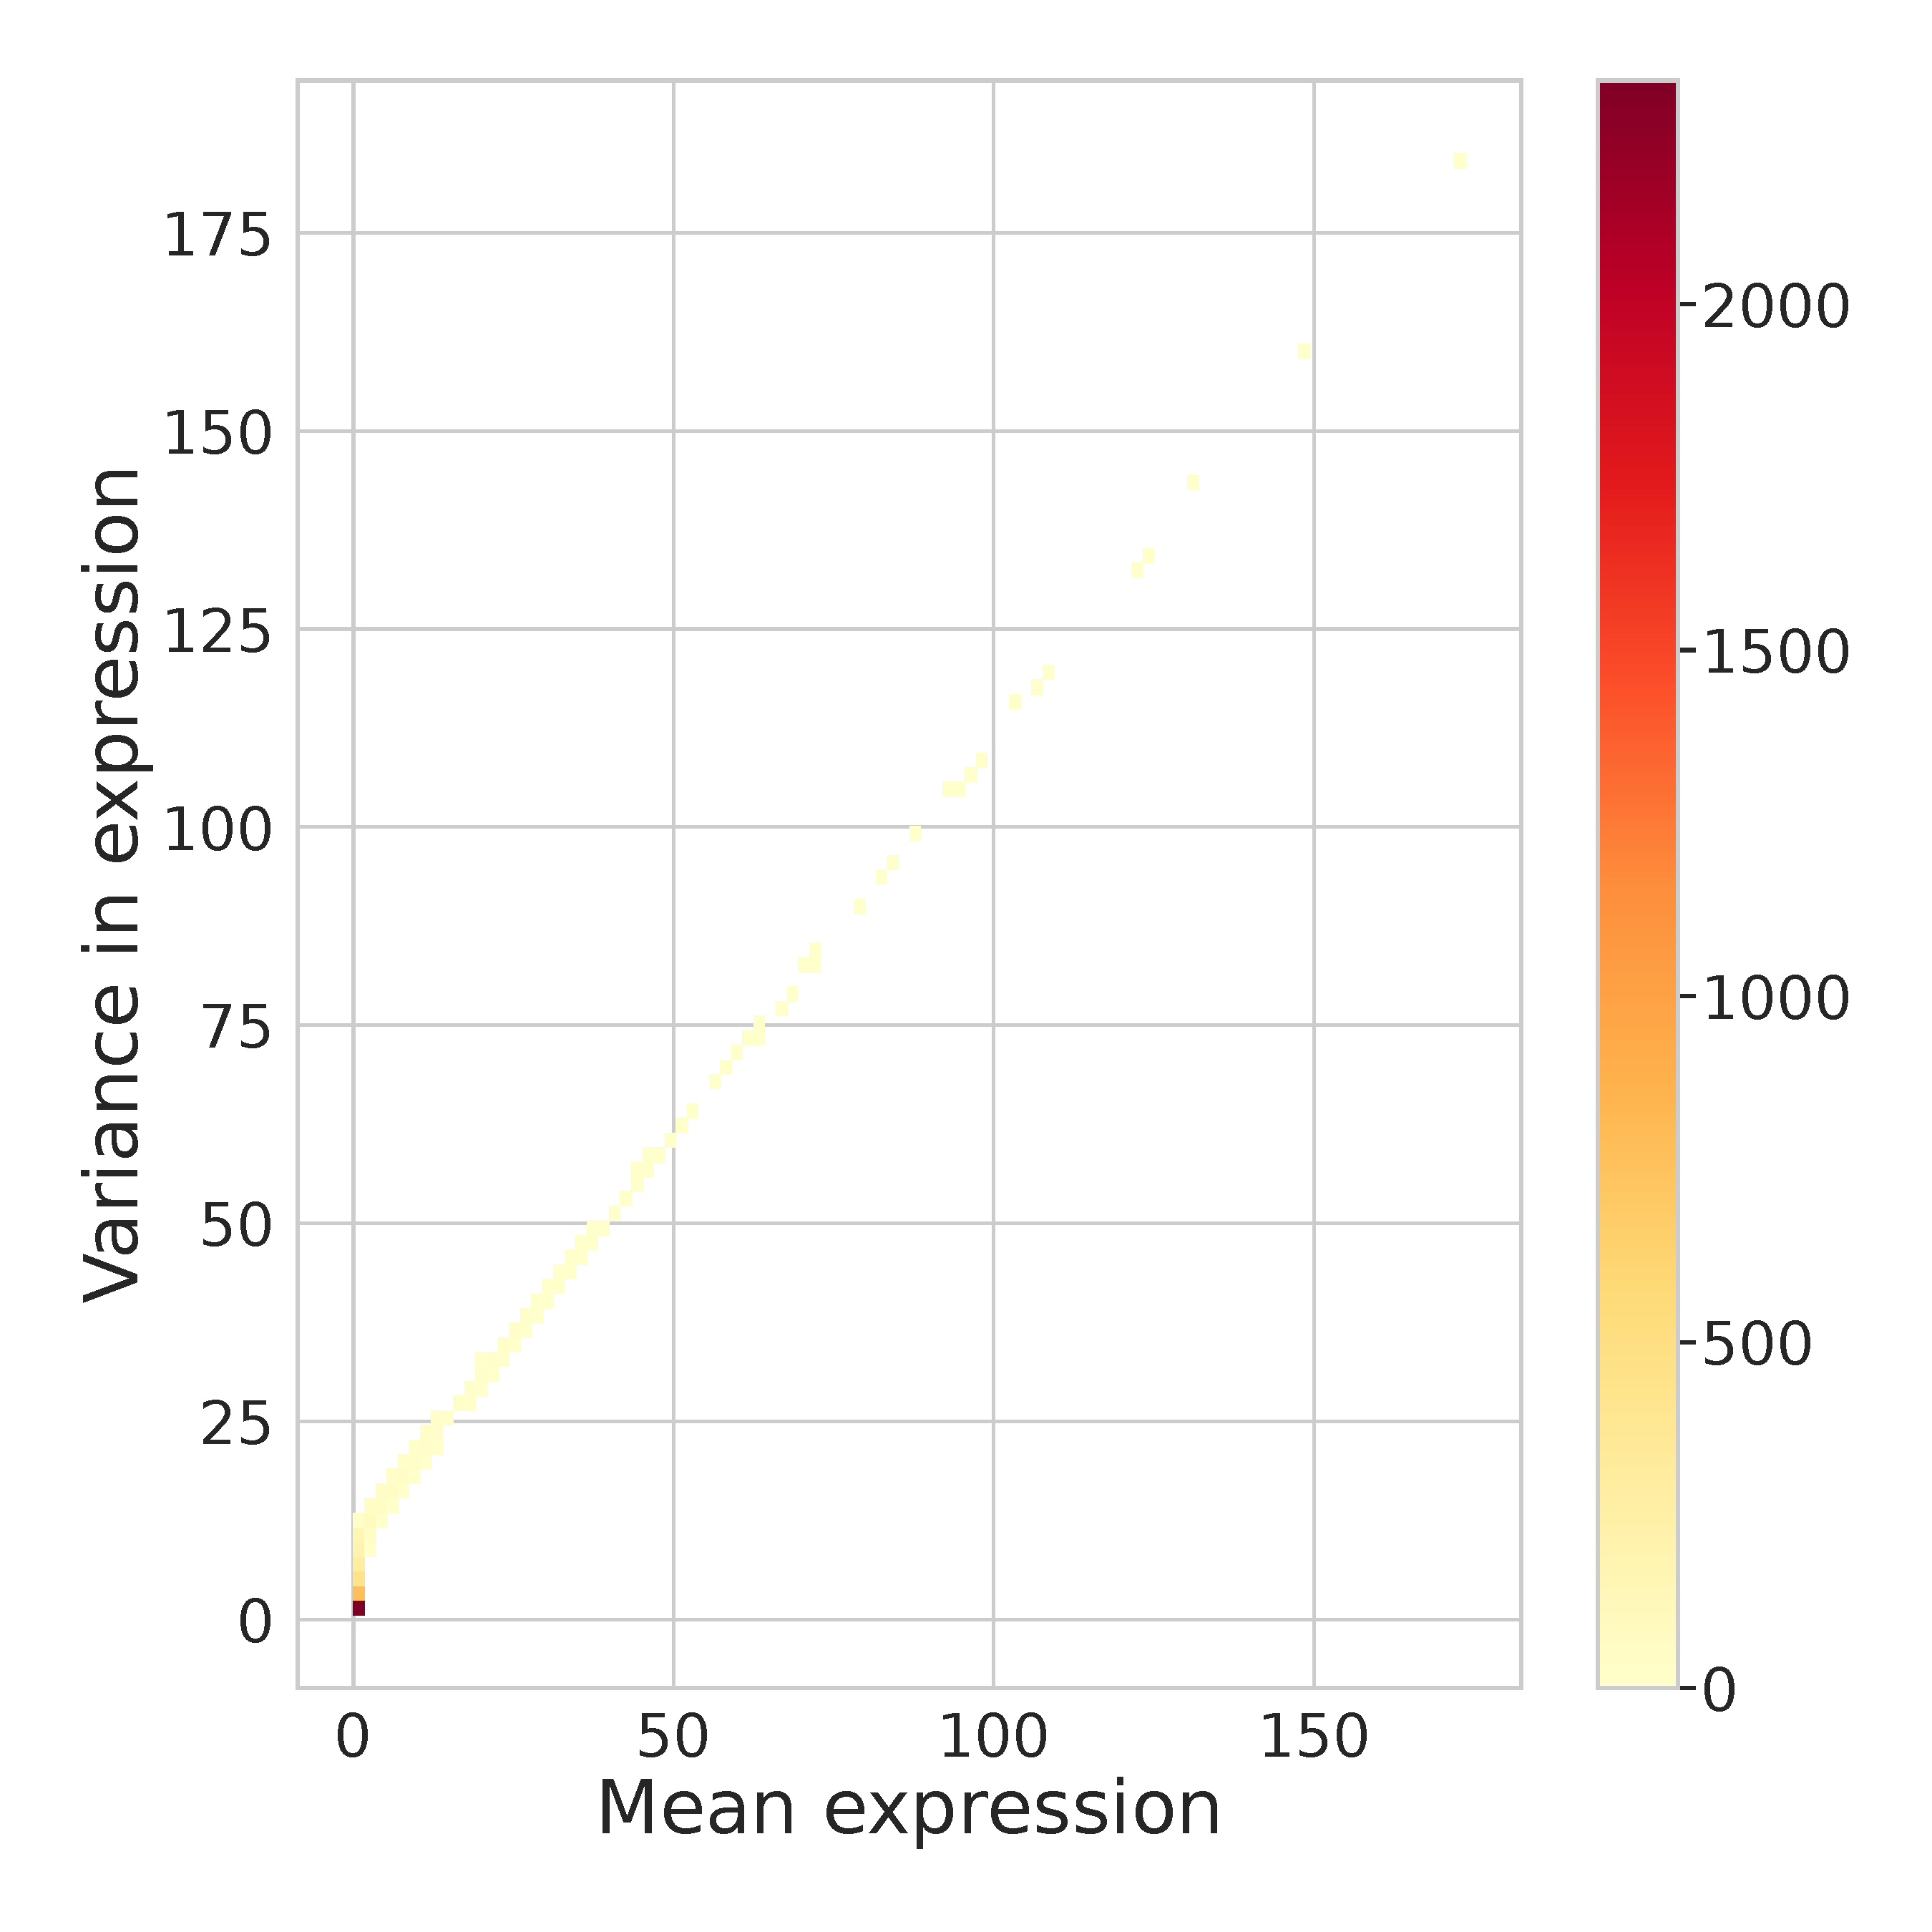
\includegraphics[width=\linewidth]{Figures/04_Highly_variable_genes/2DHist-dispersions.pdf}
                    \caption{Distribution}
                \end{figure}
            \end{column}
        \end{columns}
        \framebreak

        \begin{figure}
            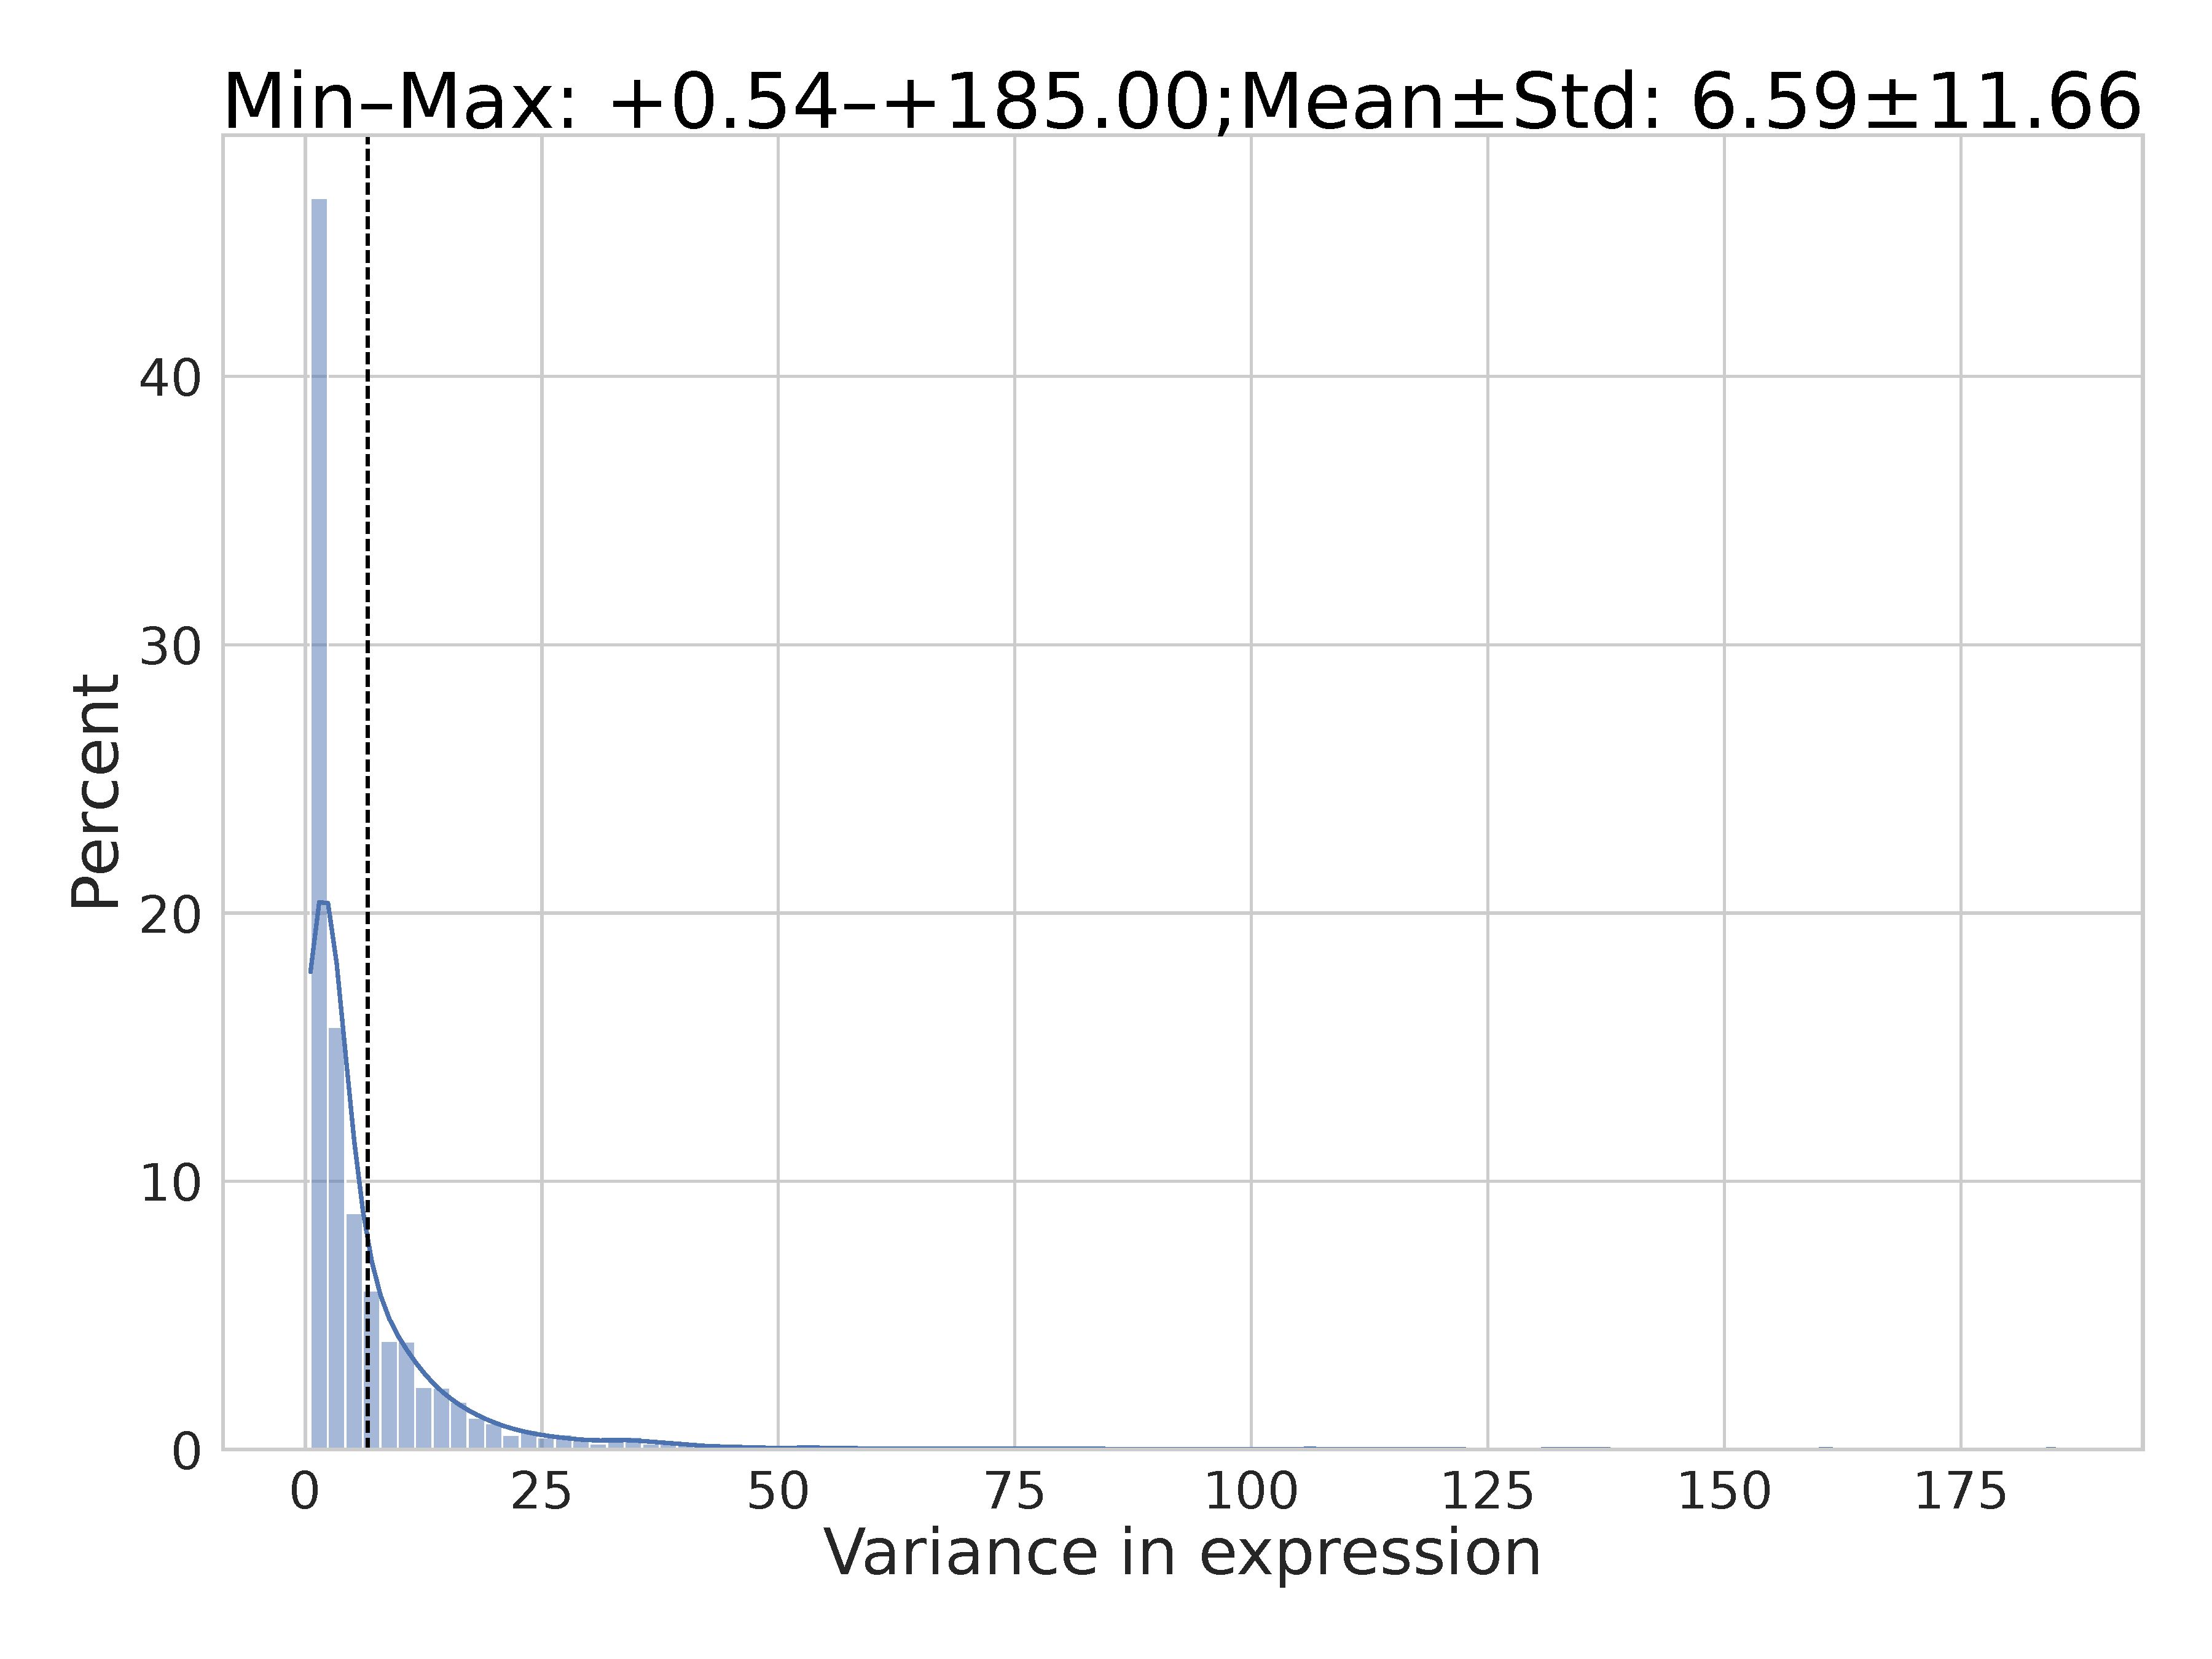
\includegraphics[width=0.7 \linewidth]{Figures/04_Highly_variable_genes/Distribution-dispersions.pdf}
            \caption{Histogram}
        \end{figure}
    \end{frame}

    \subsection{PCA}
    \begin{frame}
        \frametitle{Explained variance}

        \begin{figure}
            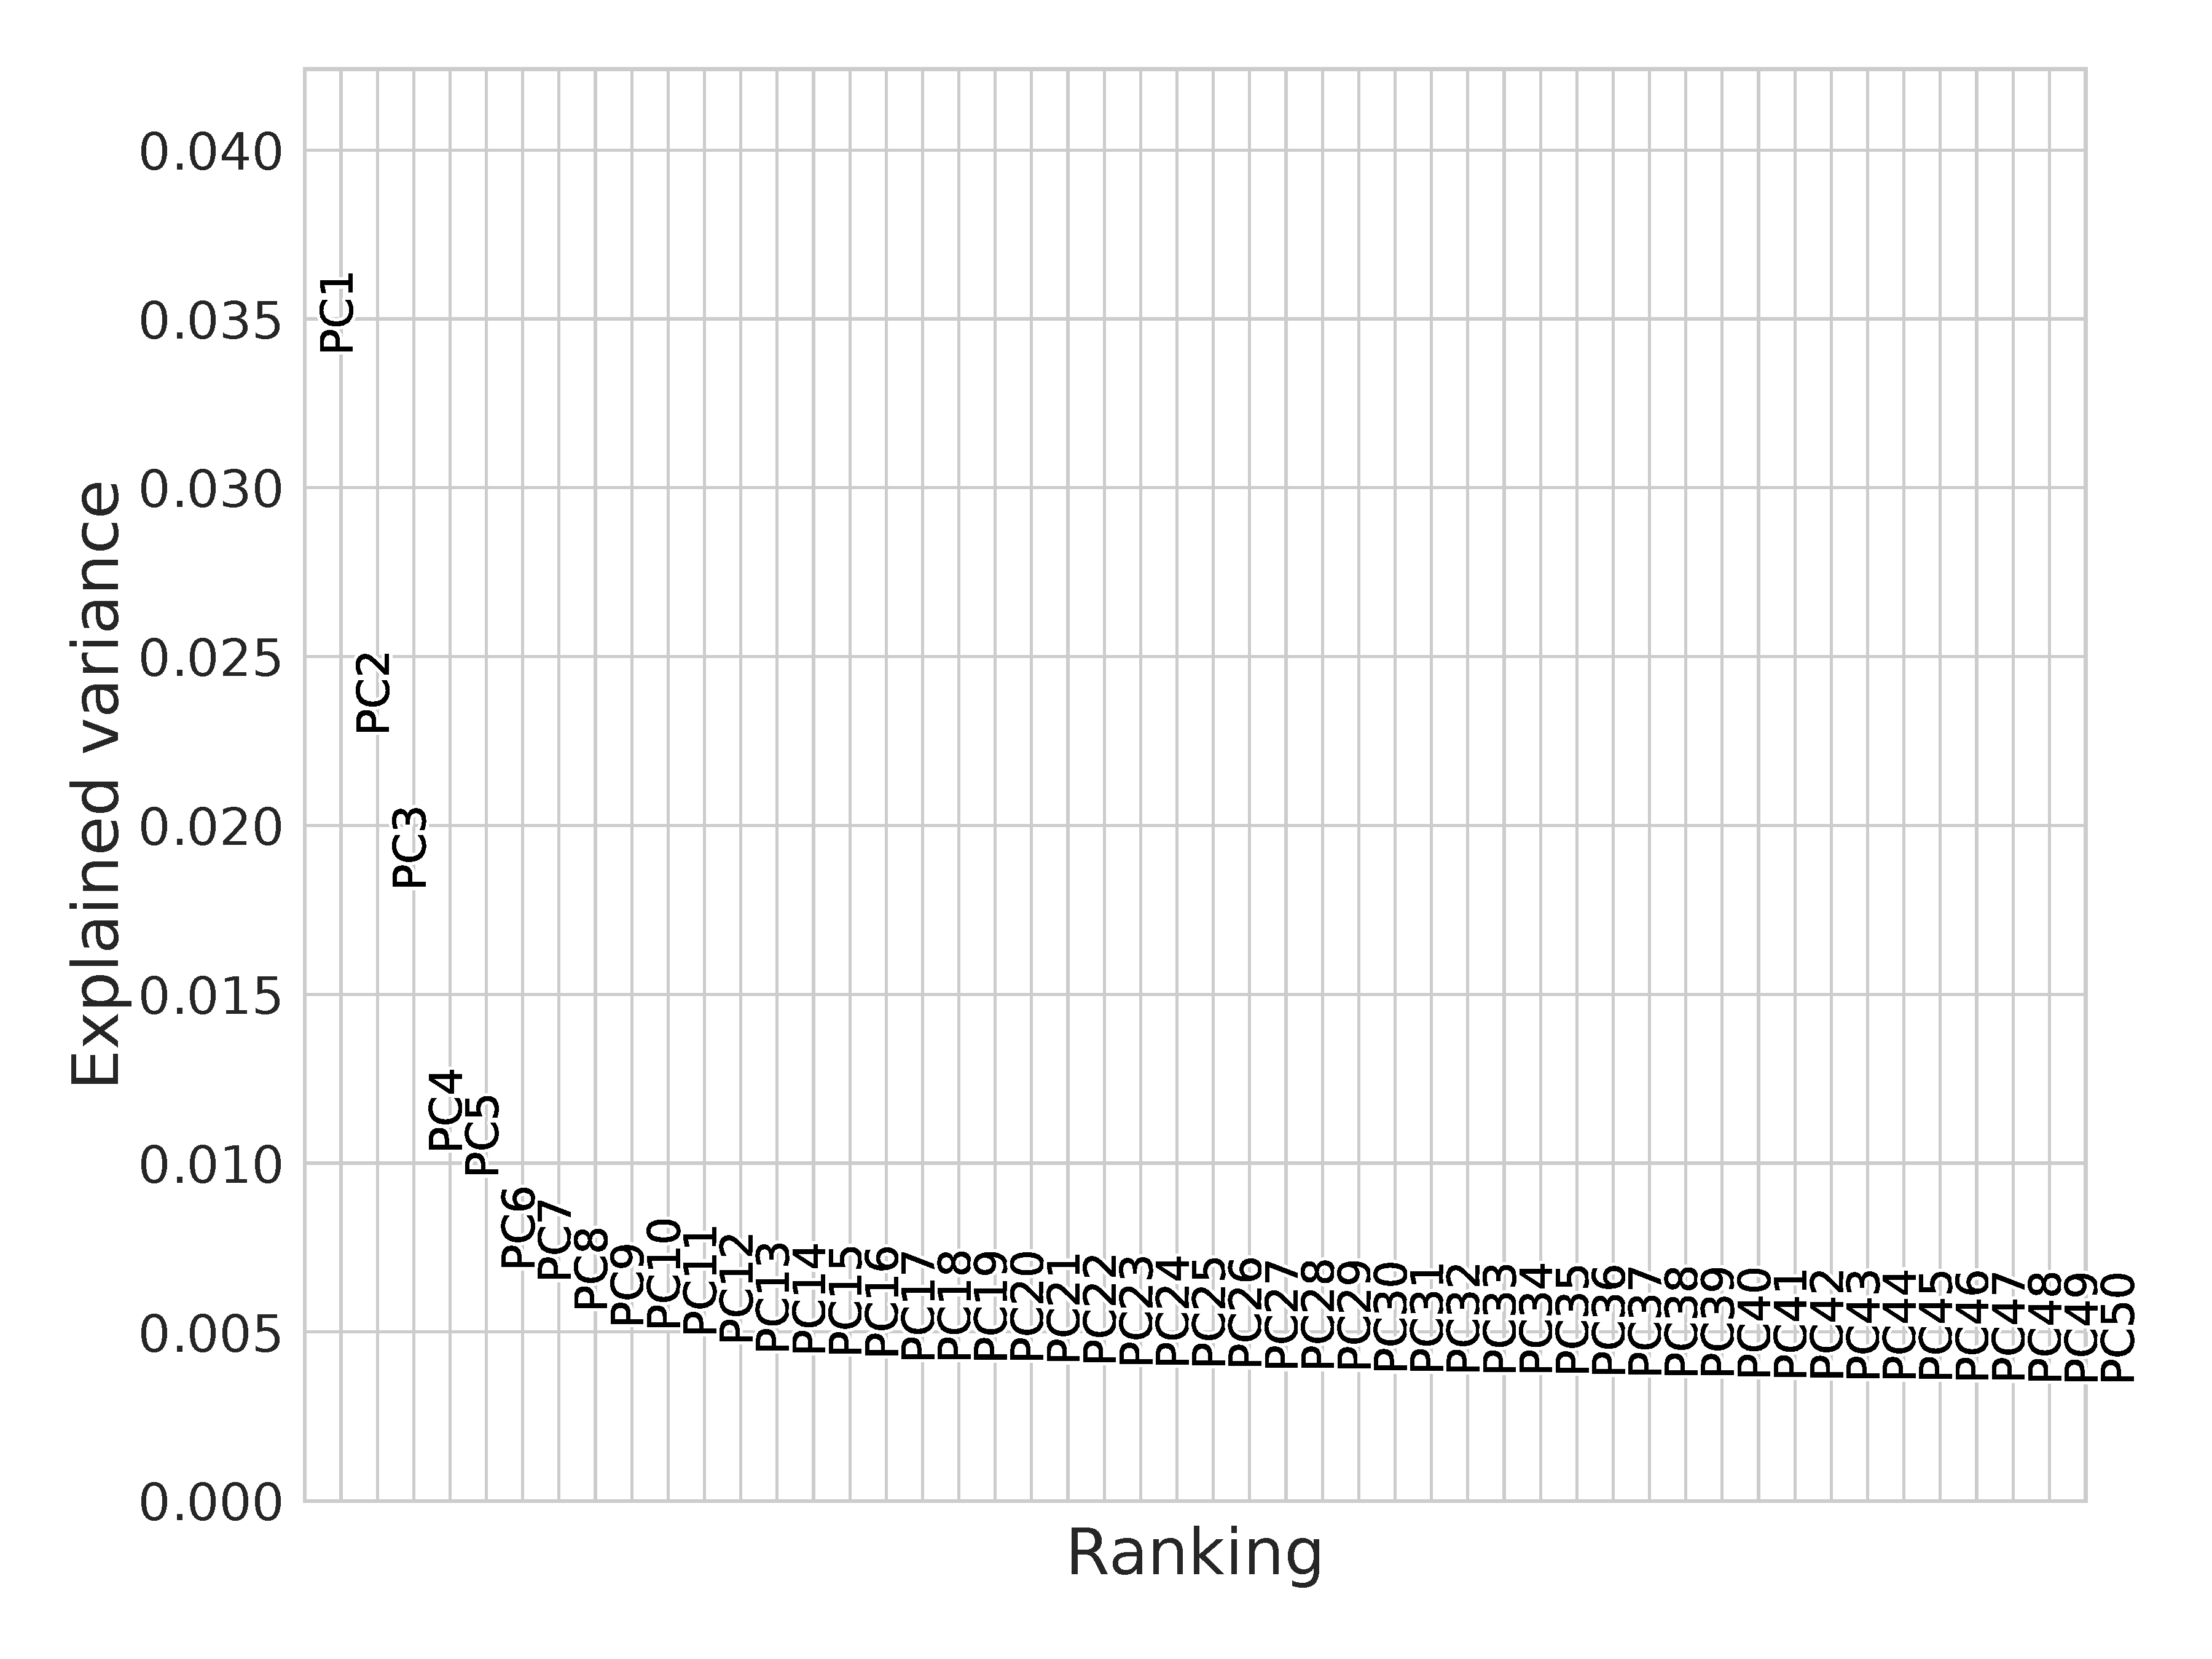
\includegraphics[width=0.7 \linewidth]{Figures/05_PCA/ExplainedVariance-Hist.pdf}
            \caption{Explained variances}
        \end{figure}
    \end{frame}

    \subsection{Clustering}
    \begin{frame}
        \frametitle{Clustering with UMAP}

        \begin{figure}
            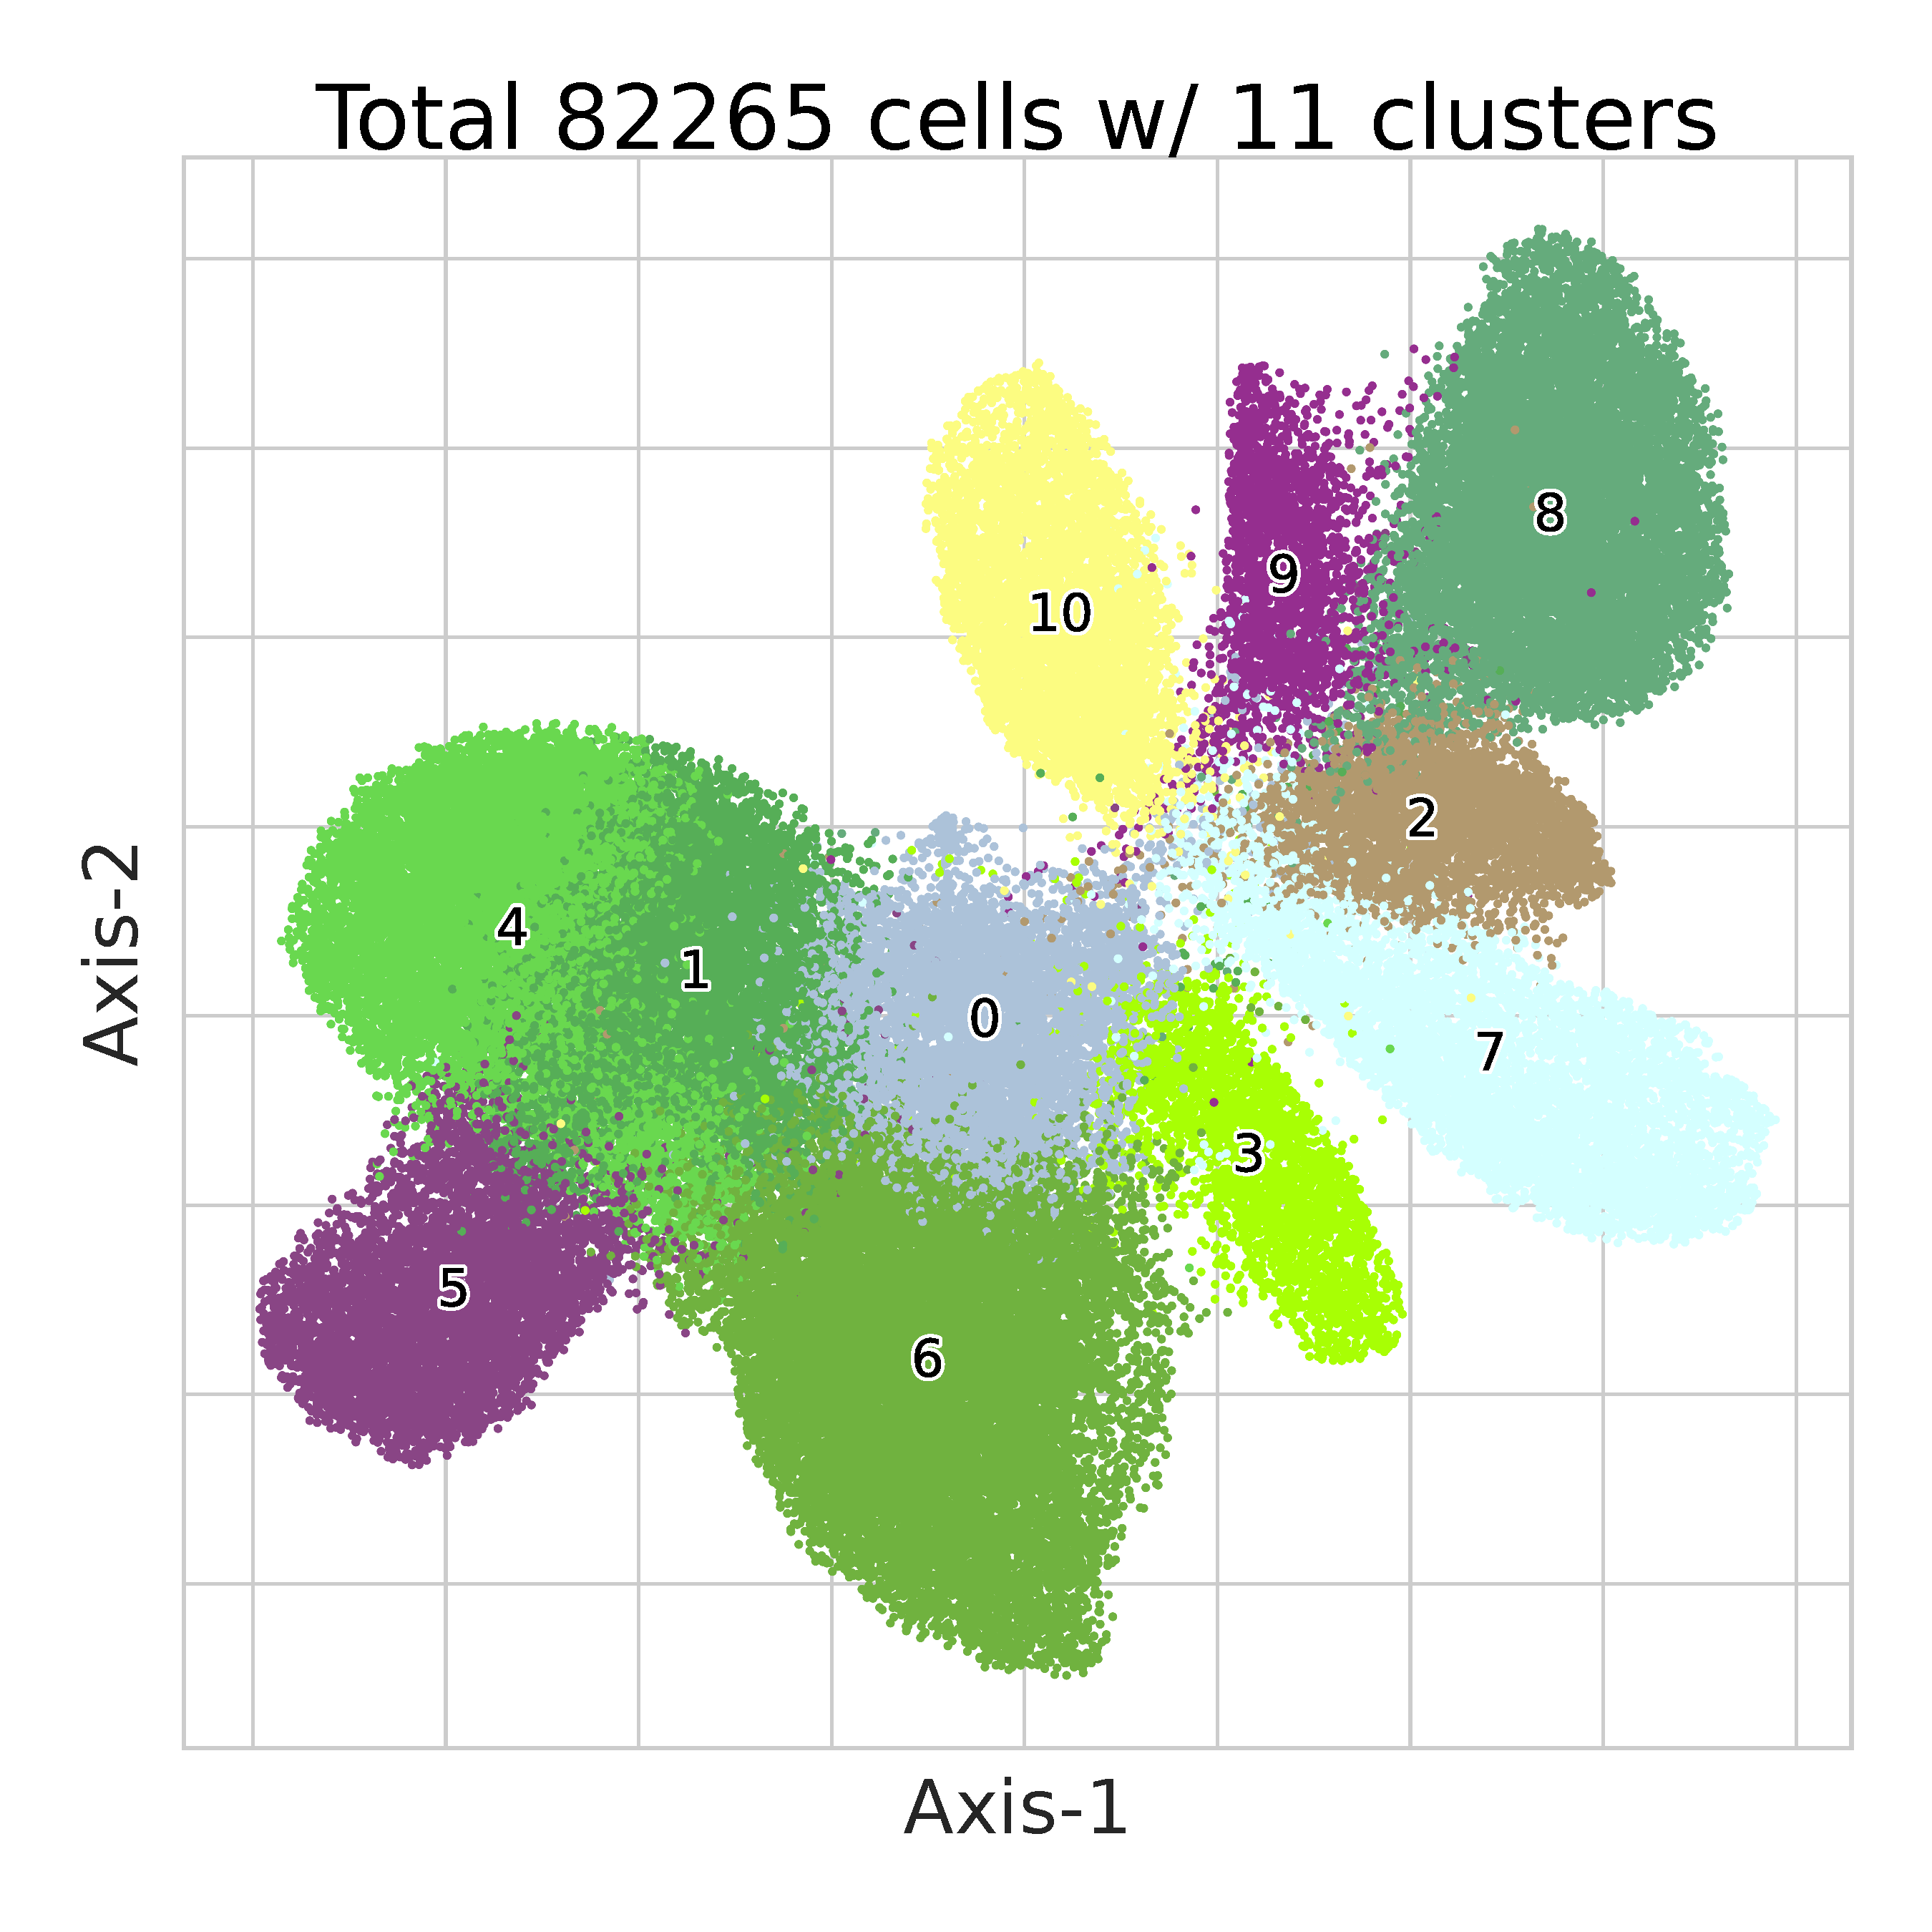
\includegraphics[width=0.5 \linewidth]{Figures/07_Clustering/Scatter.pdf}
            \caption{Clustering with UMAP}
        \end{figure}
    \end{frame}

    \begin{frame}
        \frametitle{Cells per cluster}

        \begin{columns}
            \begin{column}{0.45 \textwidth}
                \begin{figure}
                    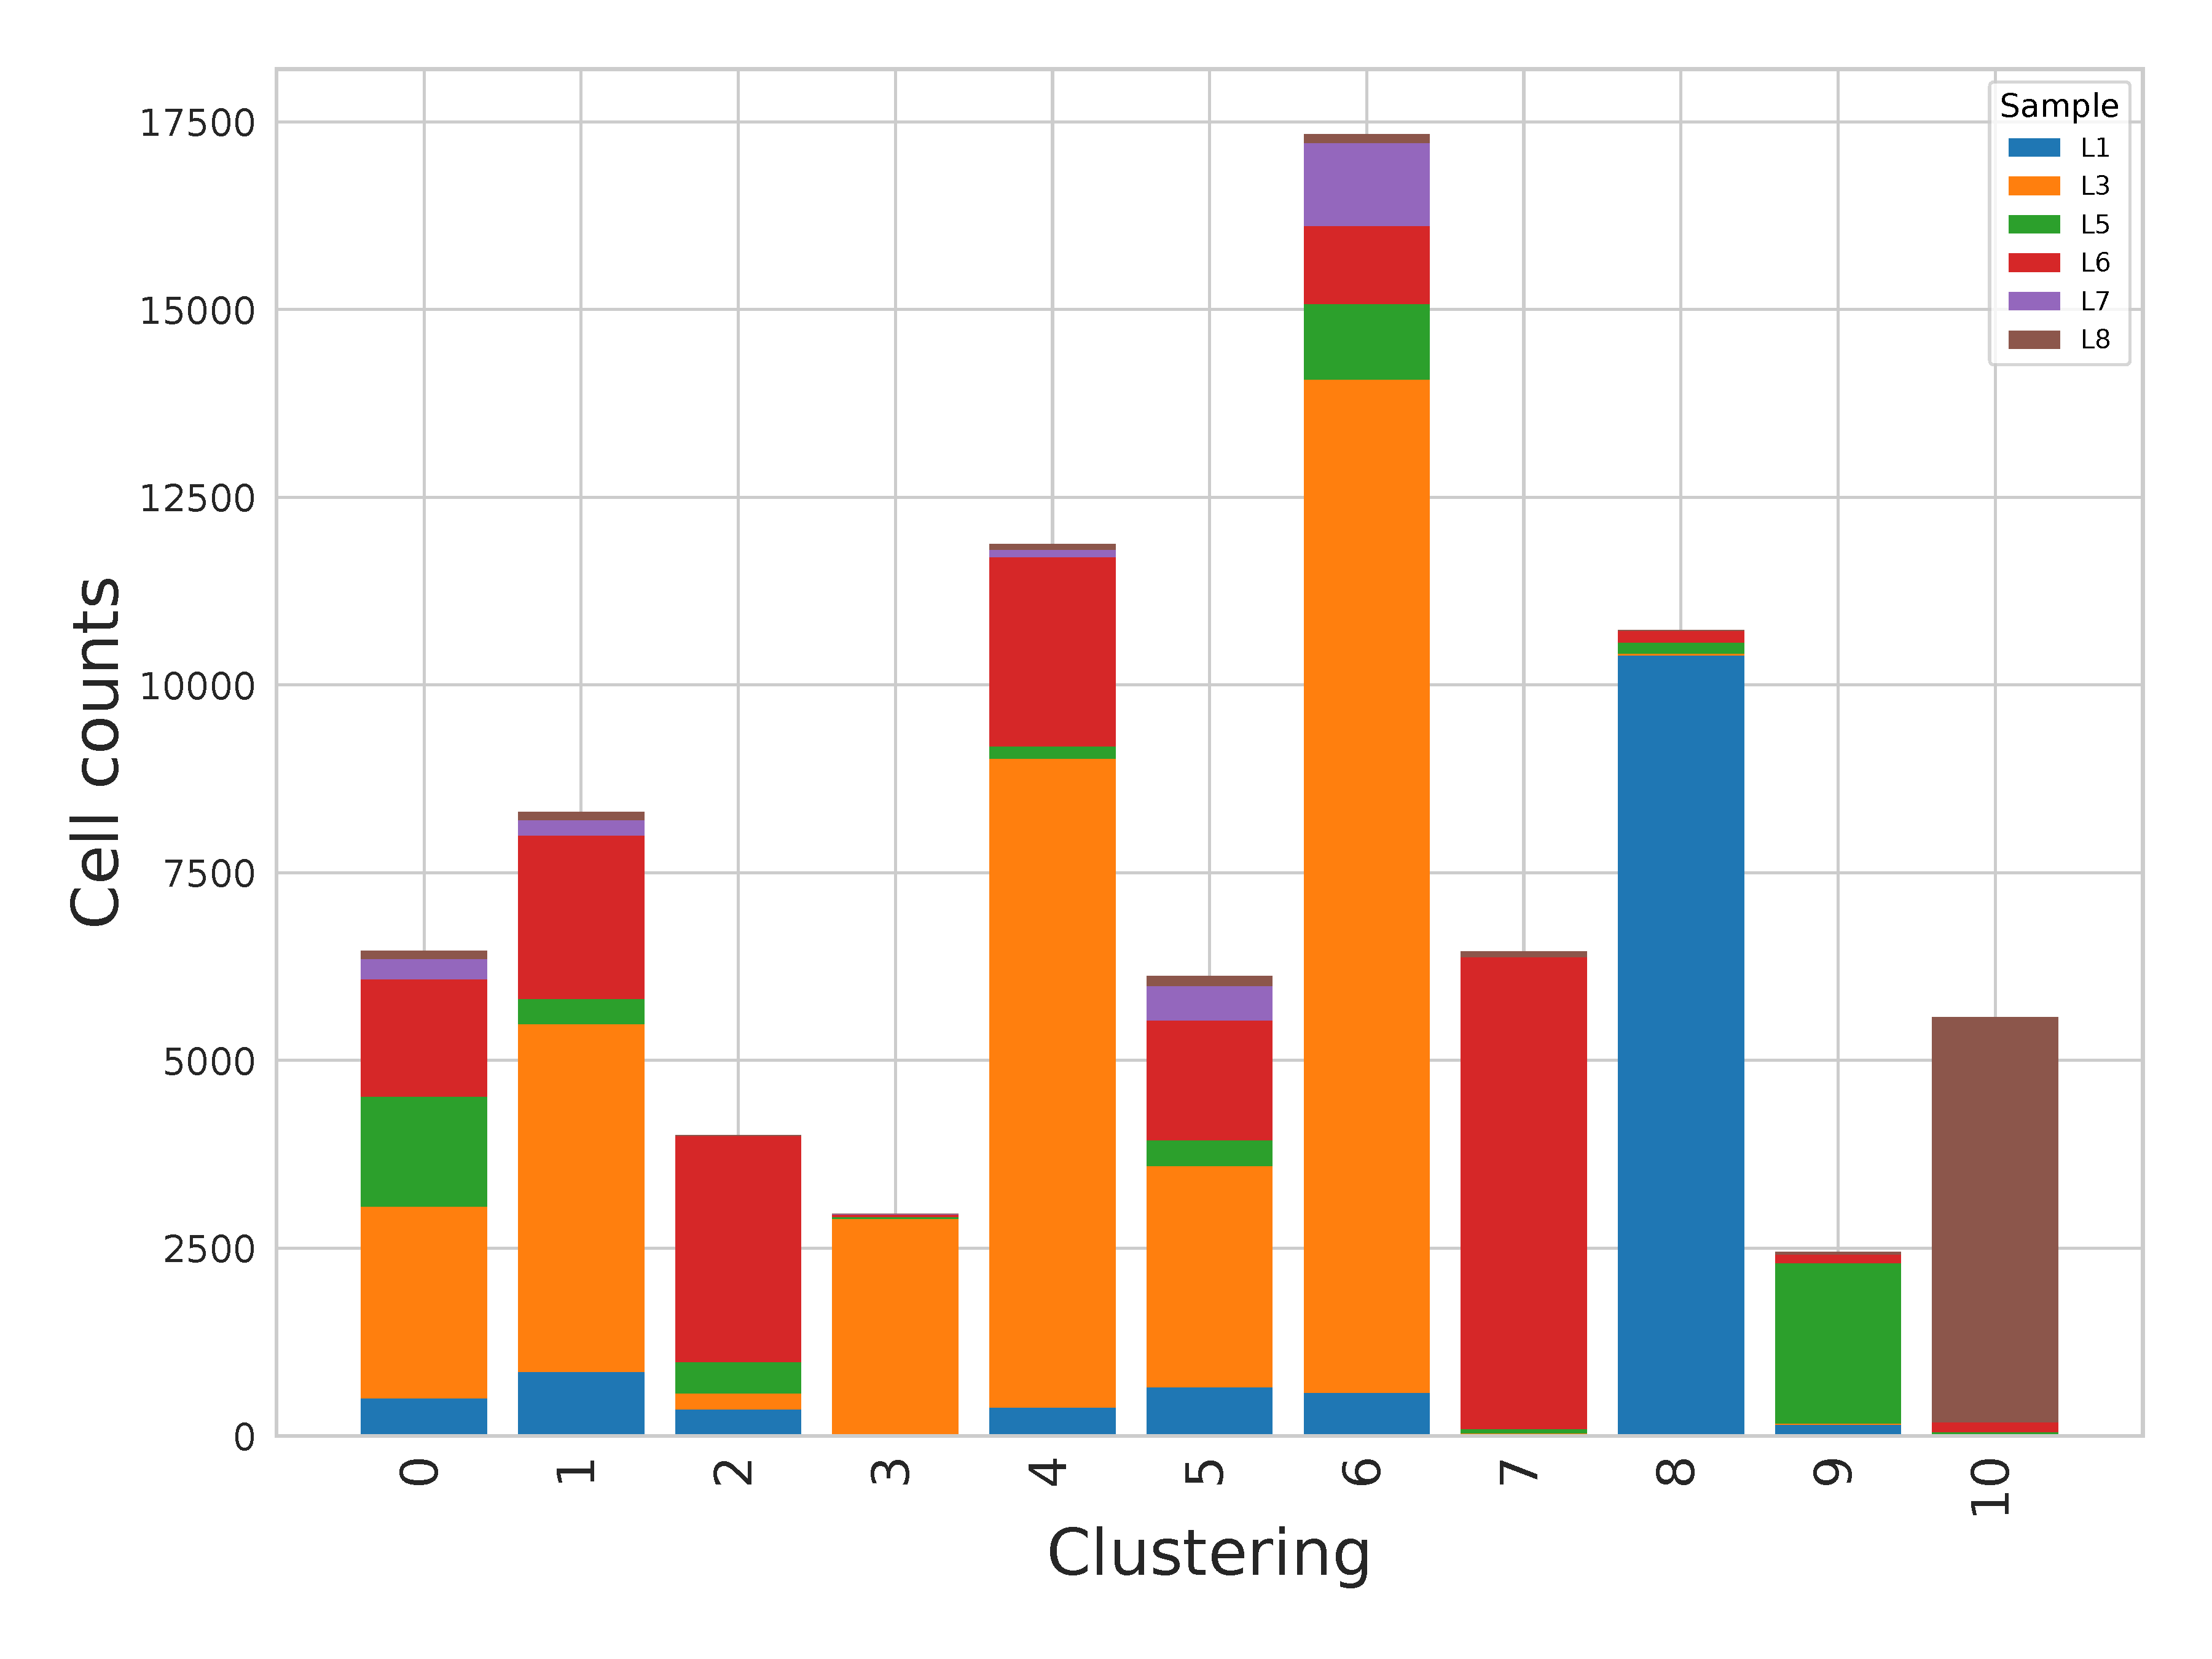
\includegraphics[width=\linewidth]{Figures/07_Clustering/Sample-Count.pdf}
                    \caption{Absolute count}
                \end{figure}
            \end{column}
            \begin{column}{0.45 \textwidth}
                \begin{figure}
                    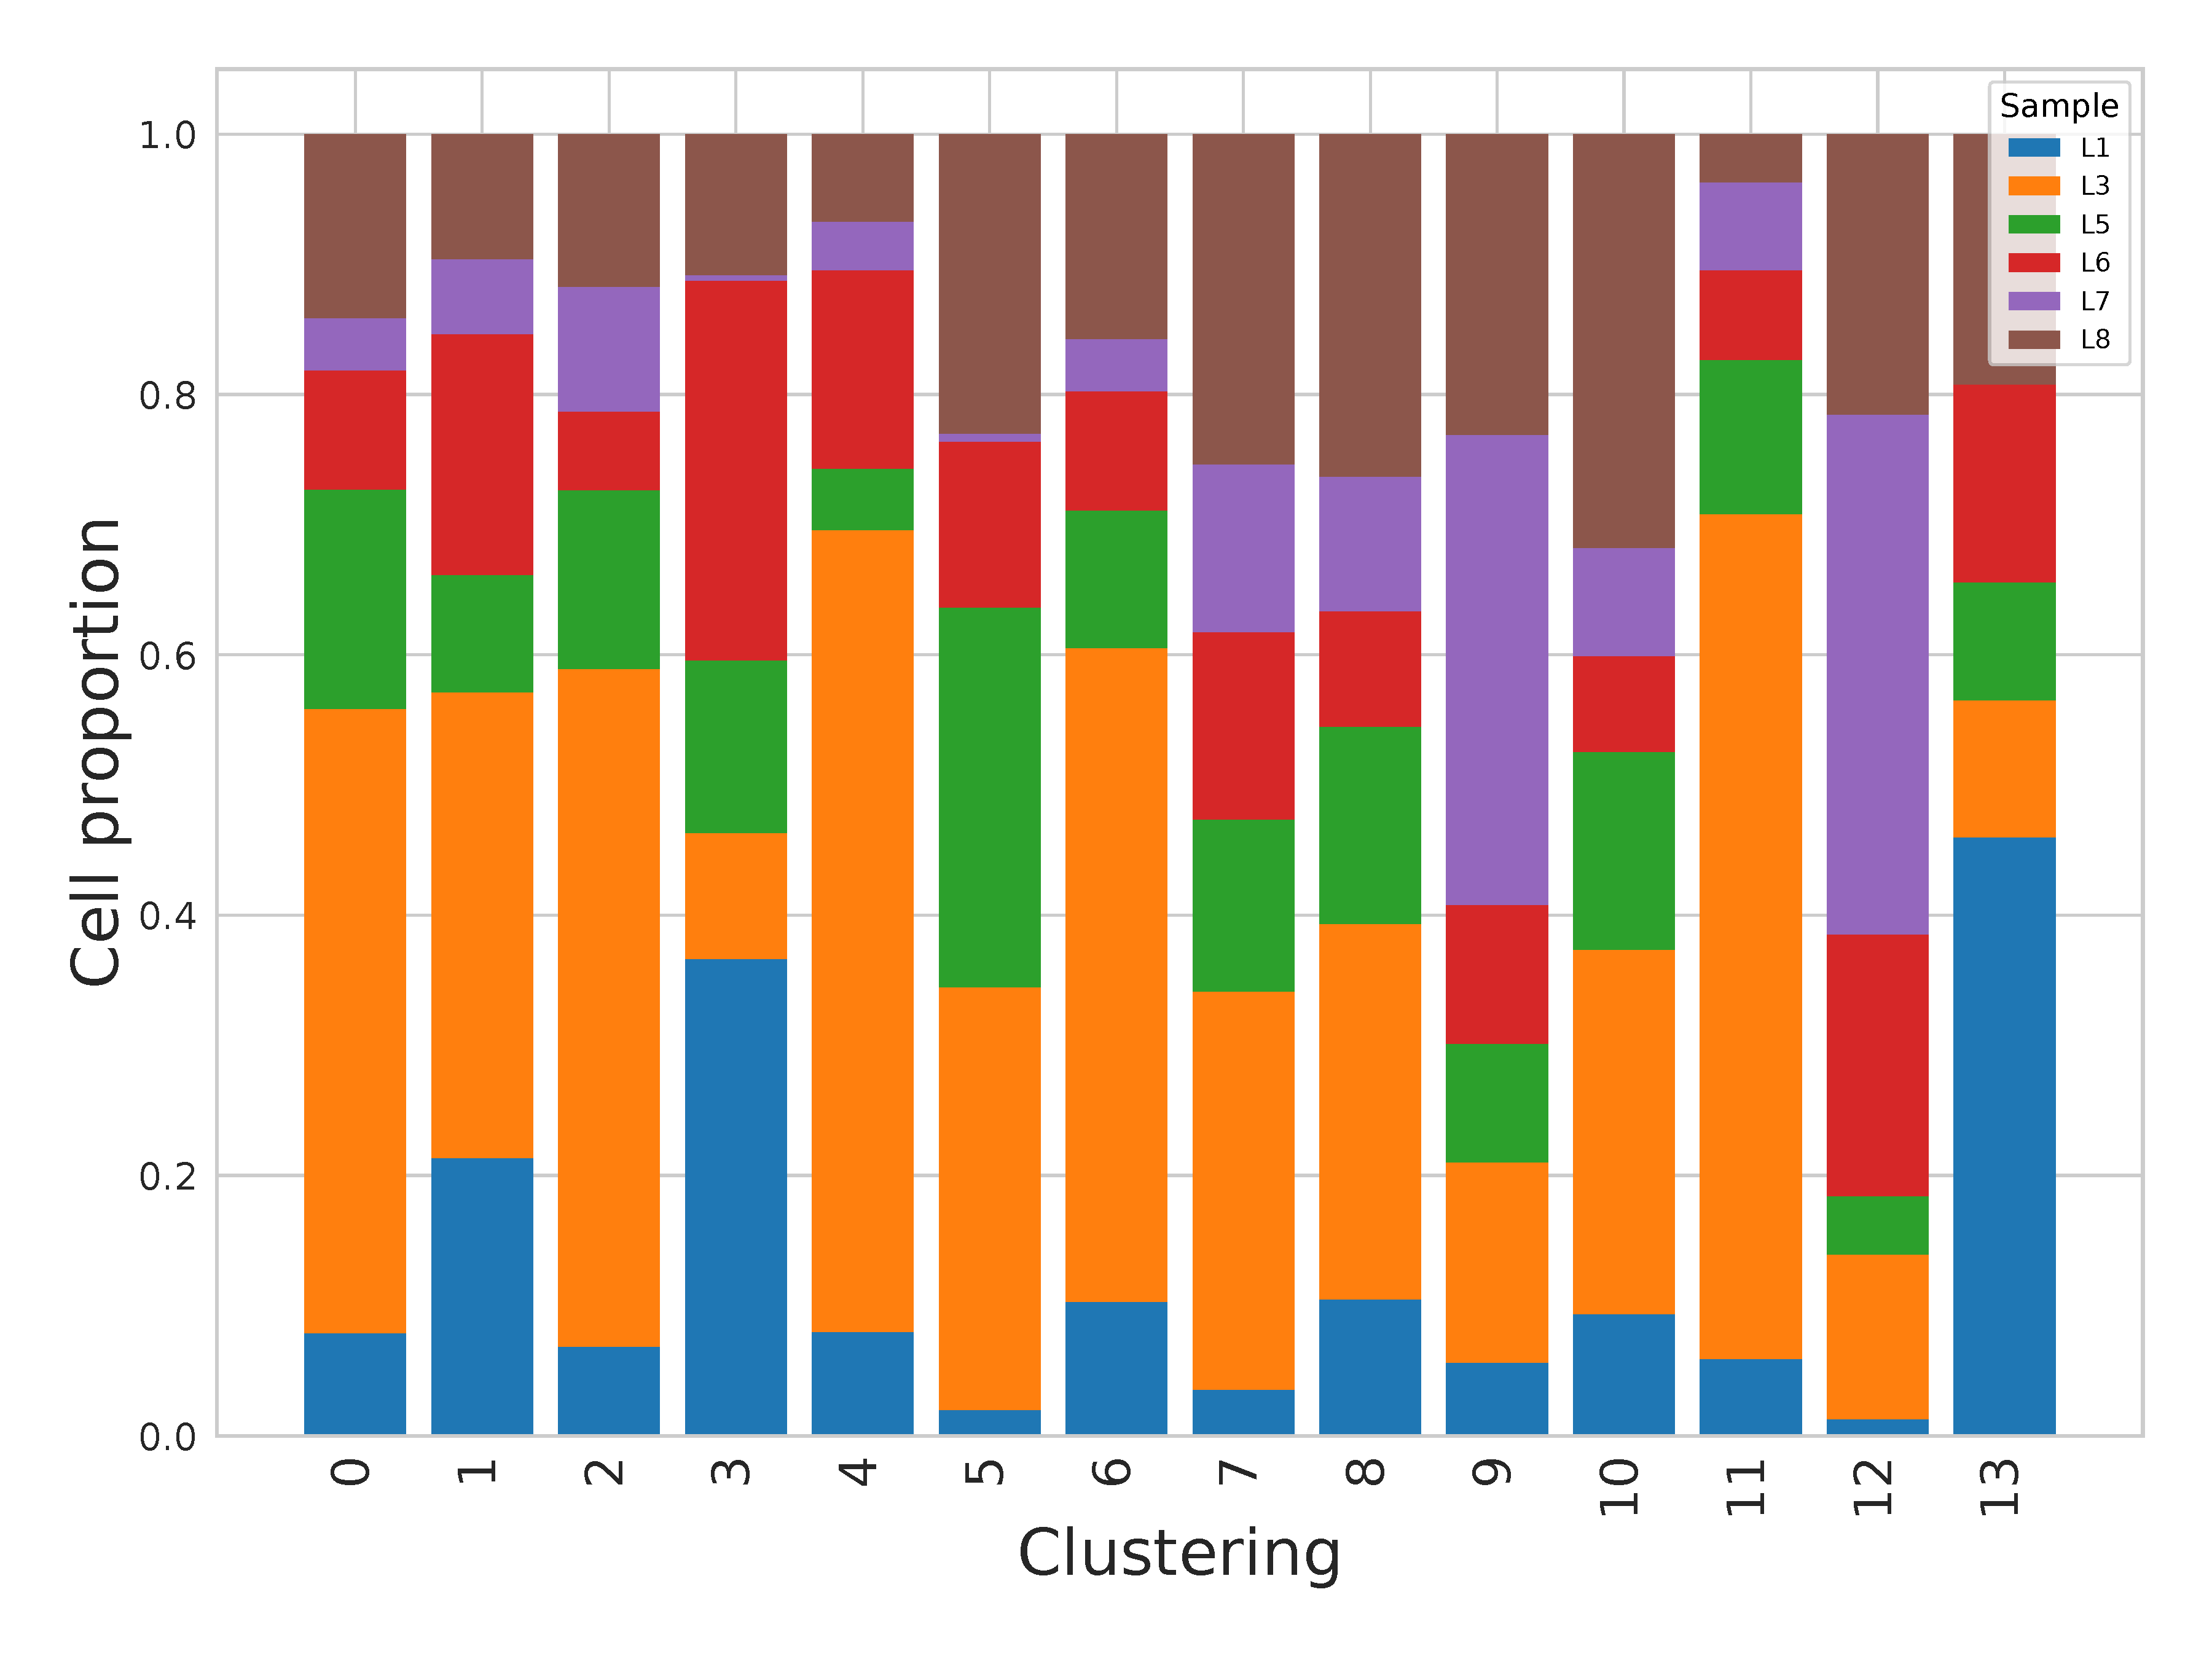
\includegraphics[width=\linewidth]{Figures/07_Clustering/Sample-Proportion.pdf}
                    \caption{Relative proportion}
                \end{figure}
            \end{column}
        \end{columns}
    \end{frame}

    \begin{frame}
        \frametitle{Cells per sample}

        \begin{columns}
            \begin{column}{0.45 \textwidth}
                \begin{figure}
                    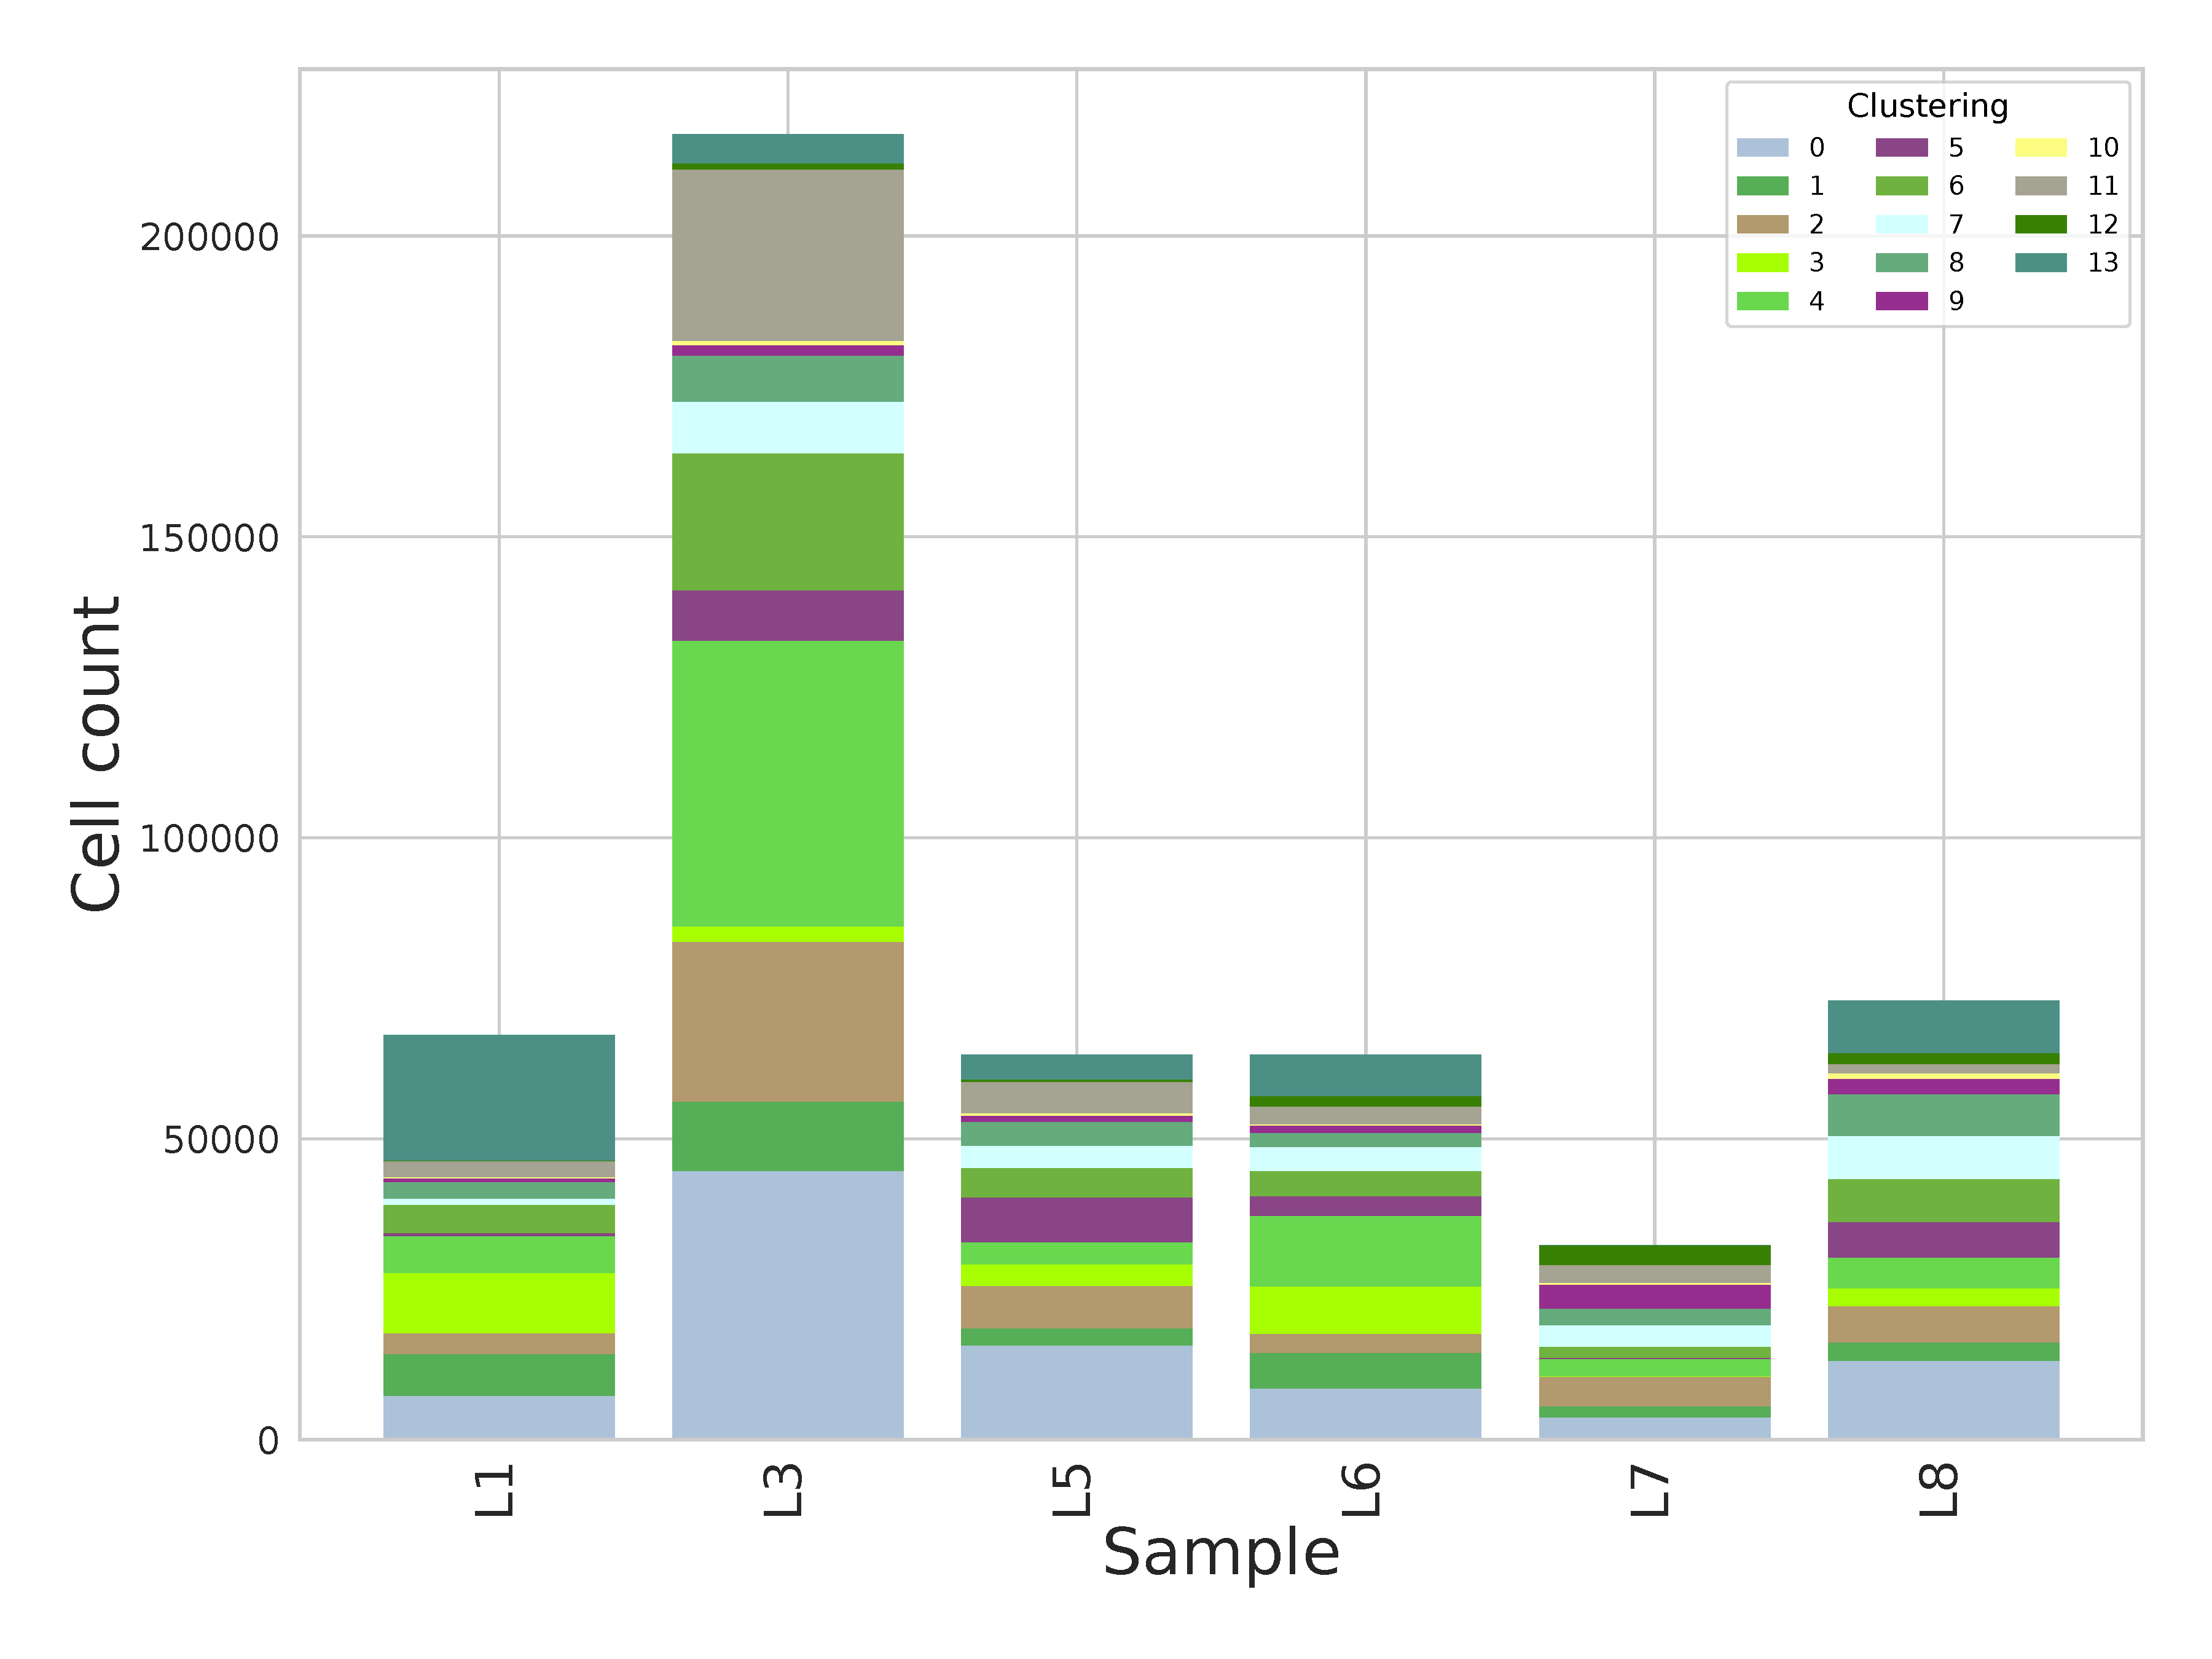
\includegraphics[width=\linewidth]{Figures/07_Clustering/Clustering-Count.pdf}
                    \caption{Absolute count}
                \end{figure}
            \end{column}
            \begin{column}{0.45 \textwidth}
                \begin{figure}
                    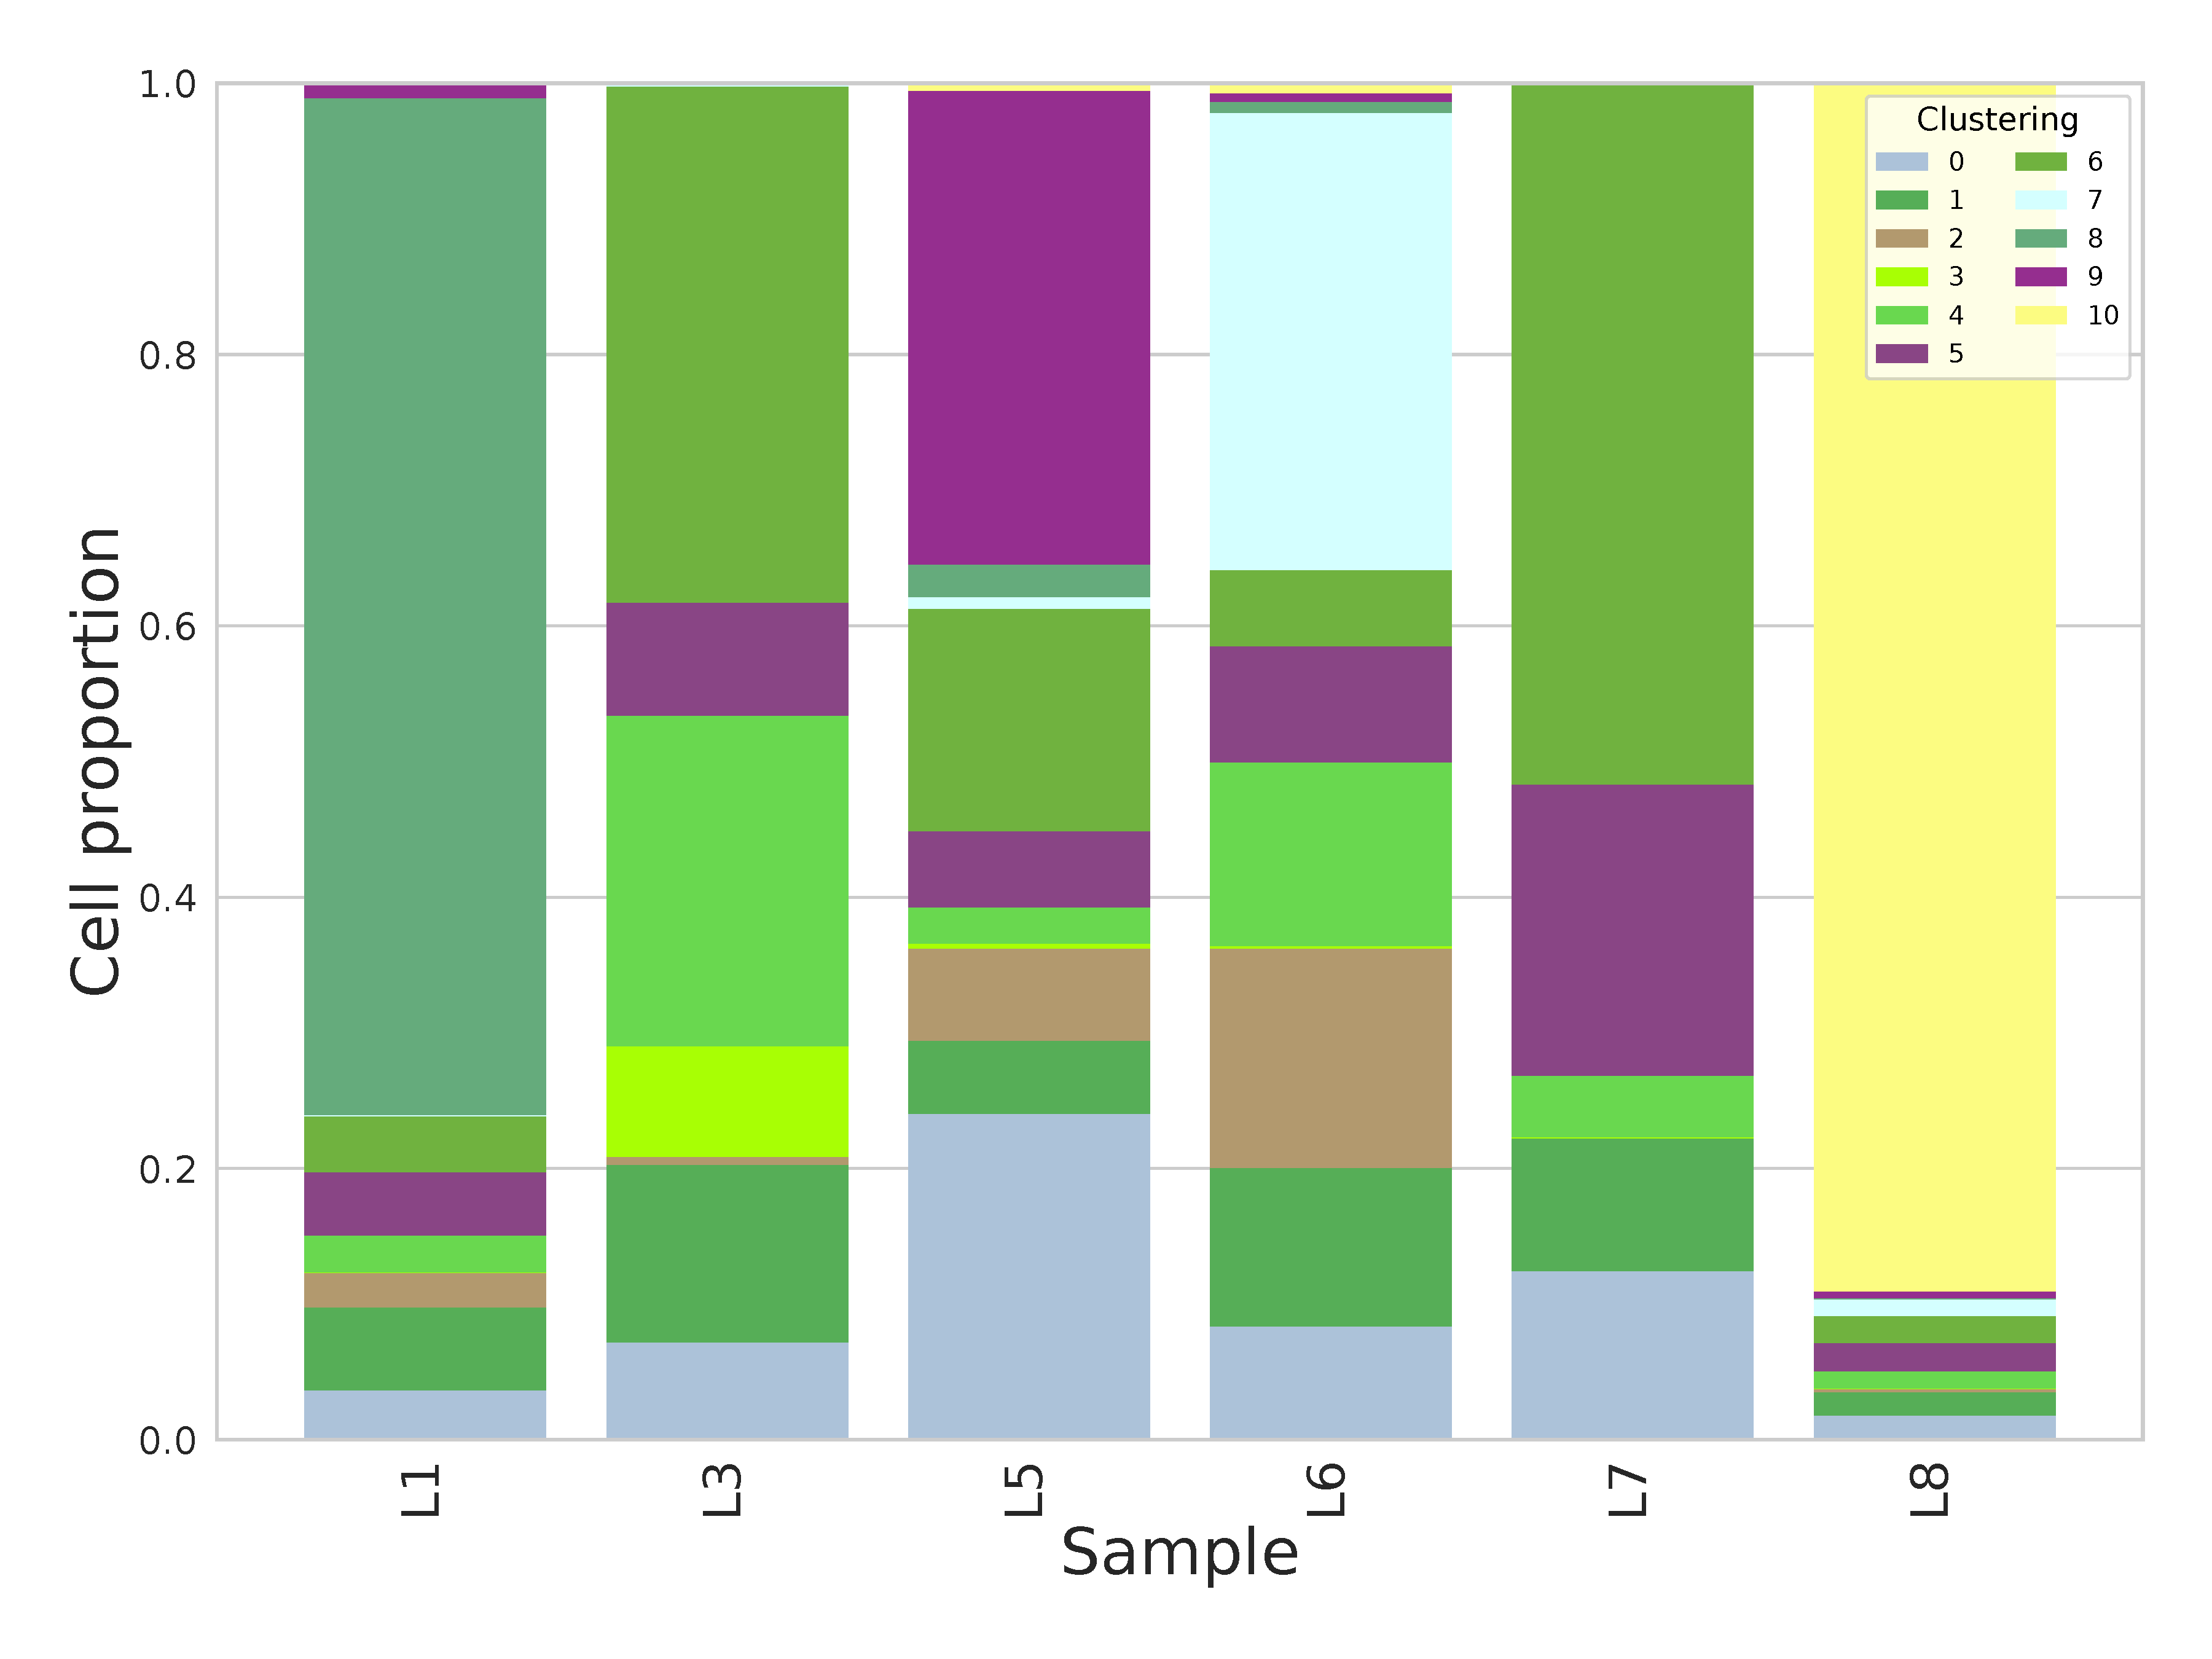
\includegraphics[width=\linewidth]{Figures/07_Clustering/Clustering-Proportion.pdf}
                    \caption{Relative proportion}
                \end{figure}
            \end{column}
        \end{columns}
    \end{frame}

    \subsection{Marker genes}
    \begin{frame}
        \frametitle{Cell type scoring}

        \begin{figure}
            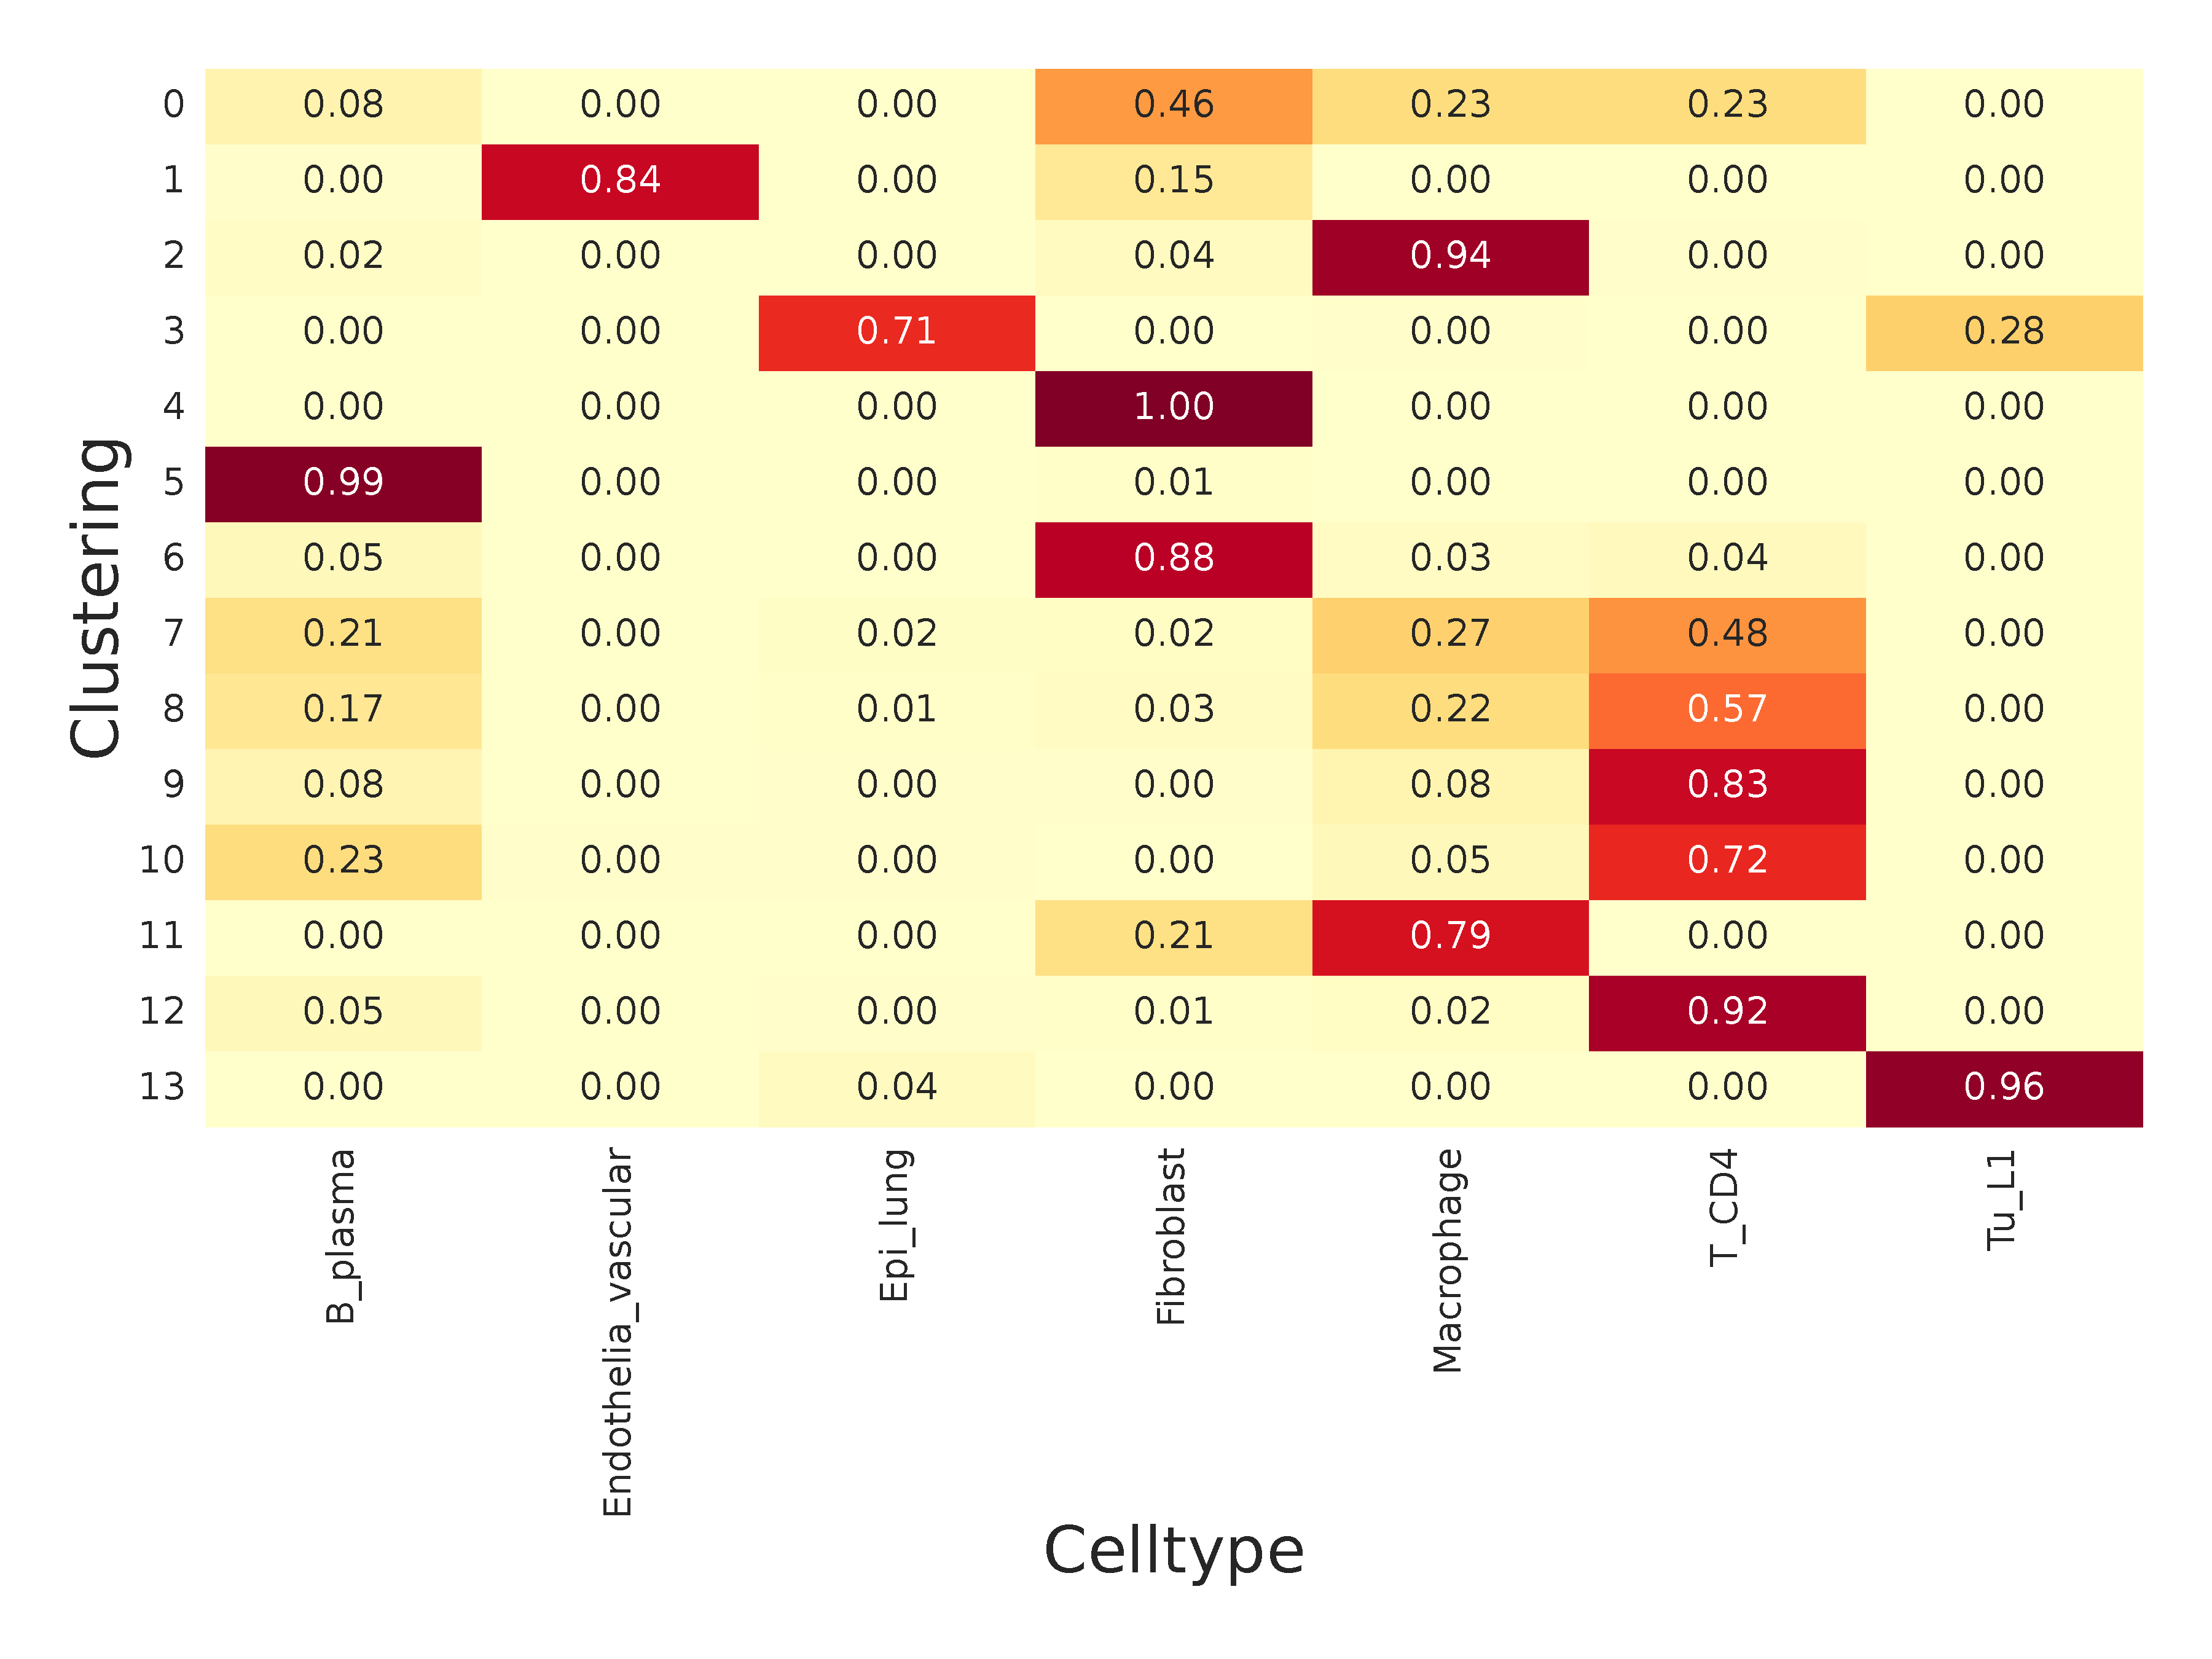
\includegraphics[width=0.7 \linewidth]{Figures/08_Marker_genes/Celltype-Score-Heatmap.pdf}
            \caption{Cell type scoring}
        \end{figure}
    \end{frame}

    \begin{frame}
        \frametitle{Cell types per cluster}

        \begin{columns}
            \begin{column}{0.45 \textwidth}
                \begin{figure}
                    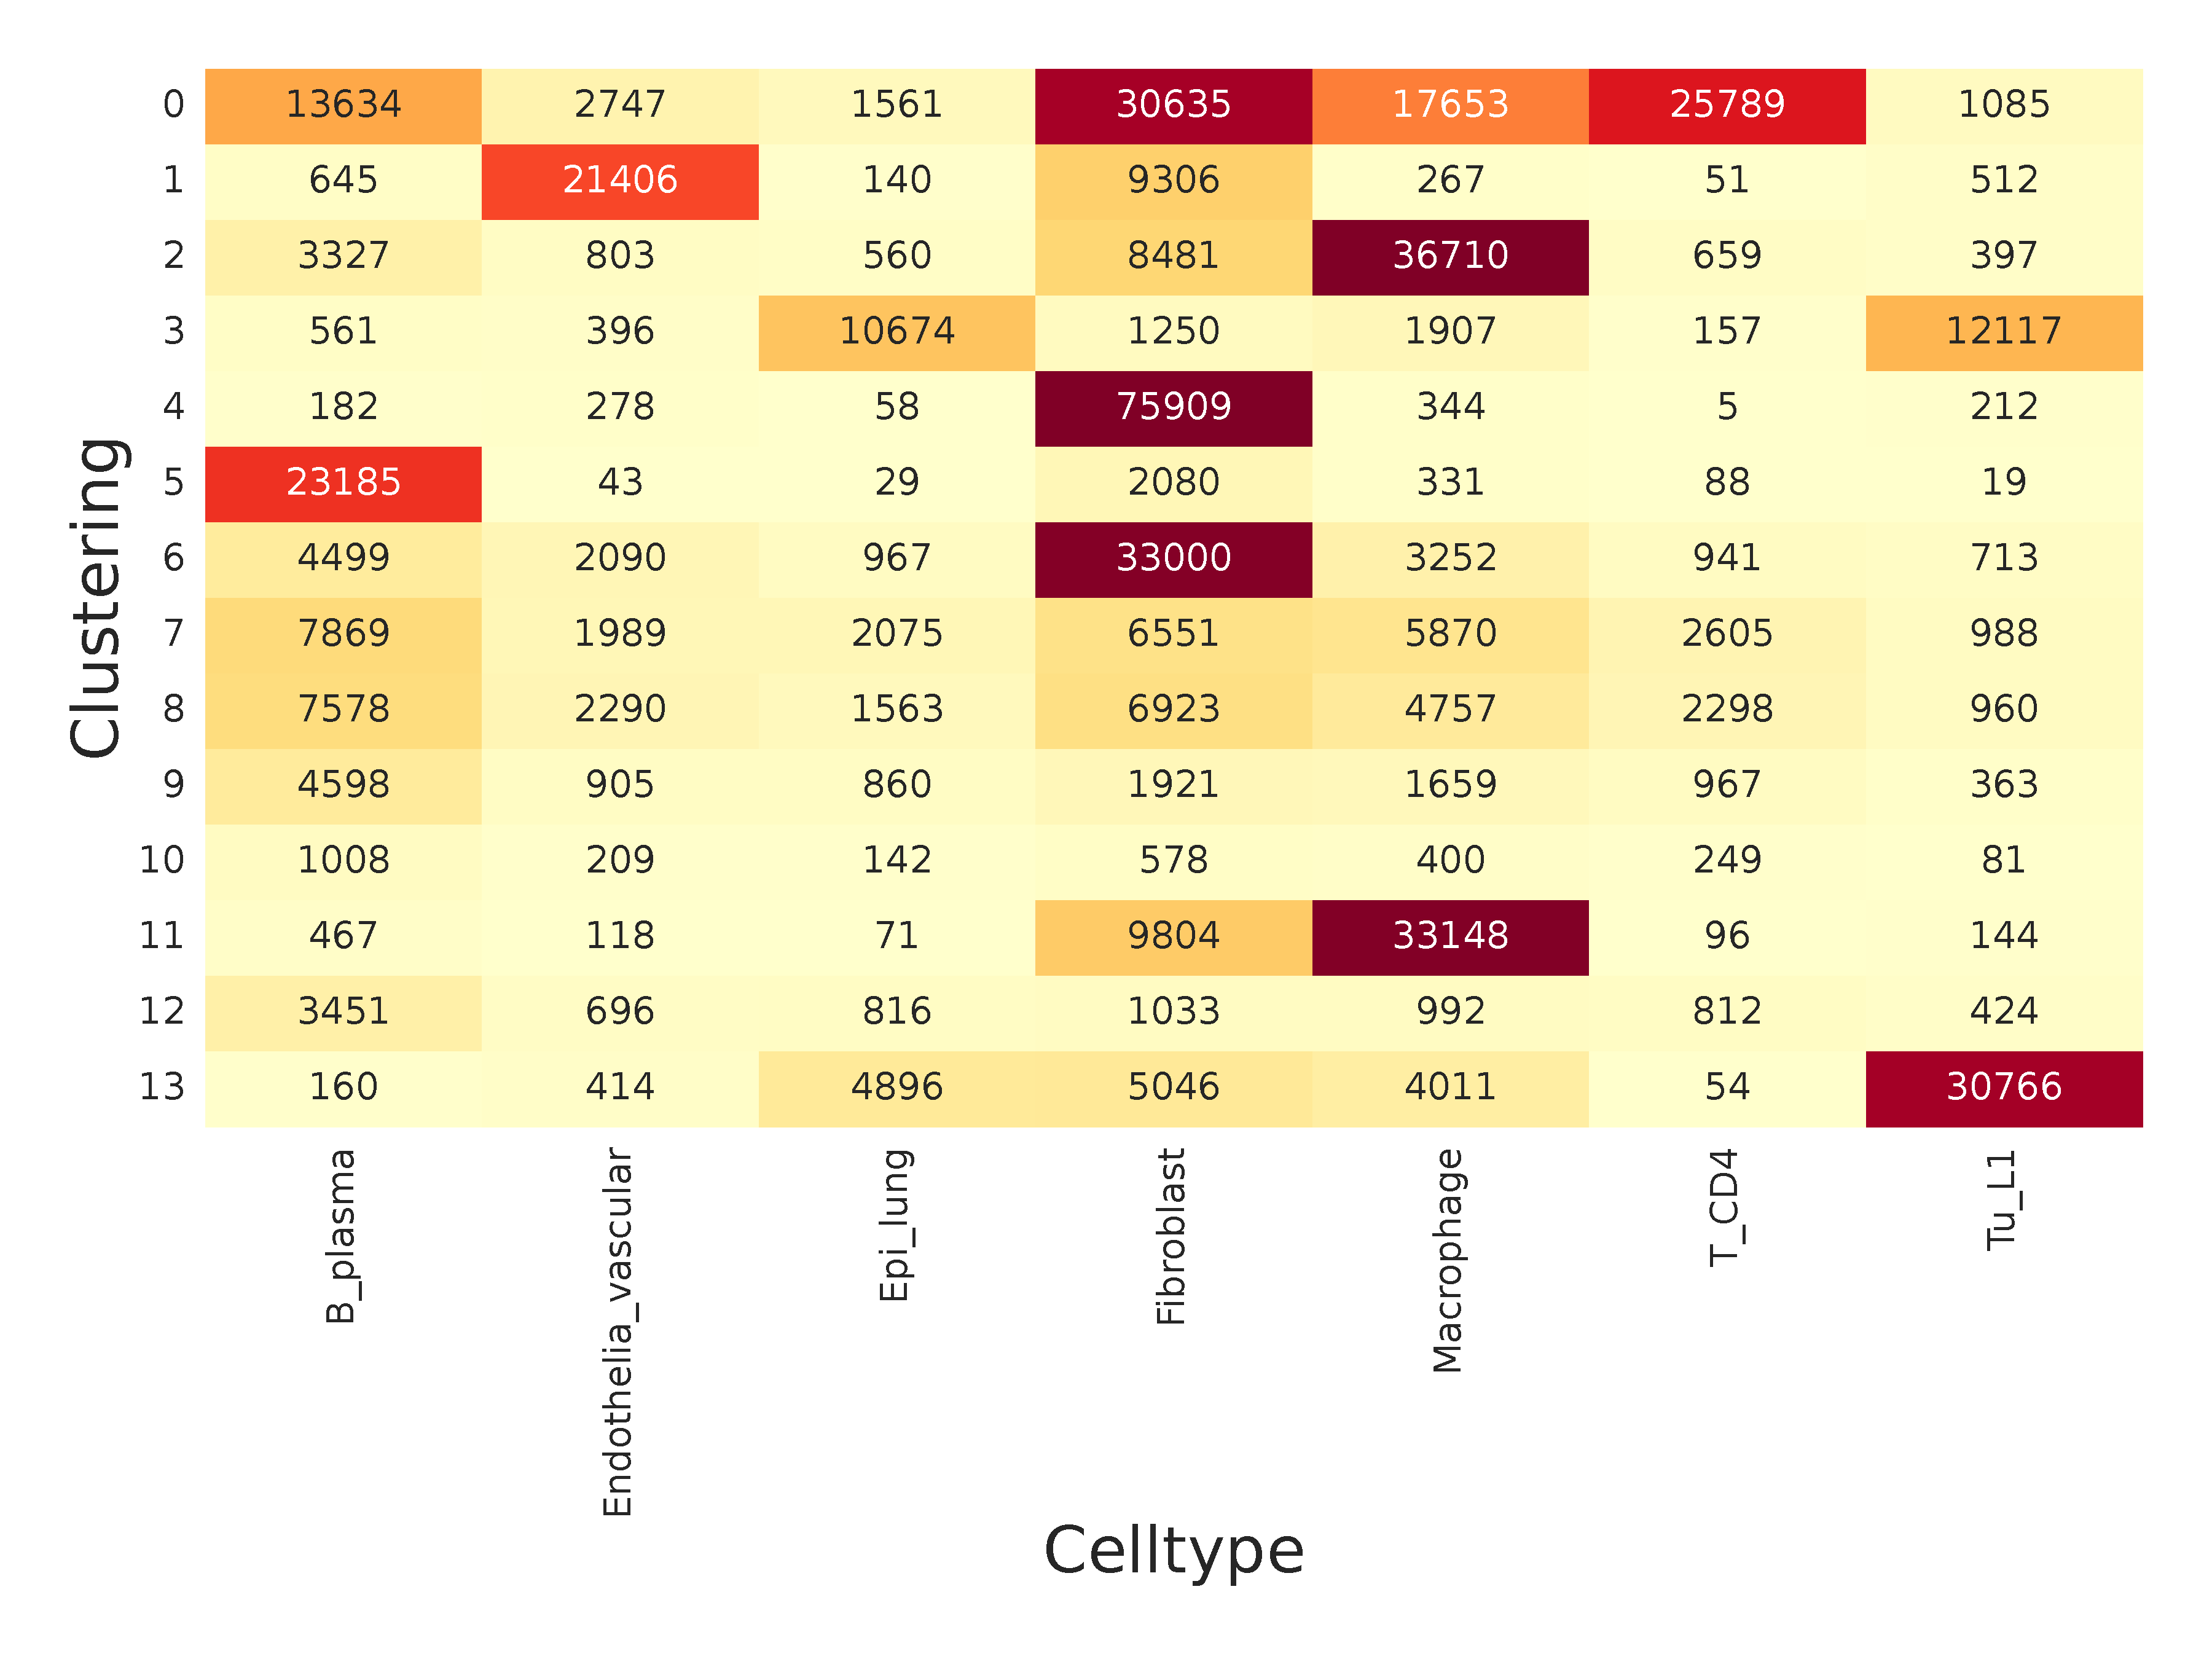
\includegraphics[width=\linewidth]{Figures/08_Marker_genes/Celltype-Count-Heatmap.pdf}
                    \caption{Absolute count}
                \end{figure}
            \end{column}
            \begin{column}{0.45 \textwidth}
                \begin{figure}
                    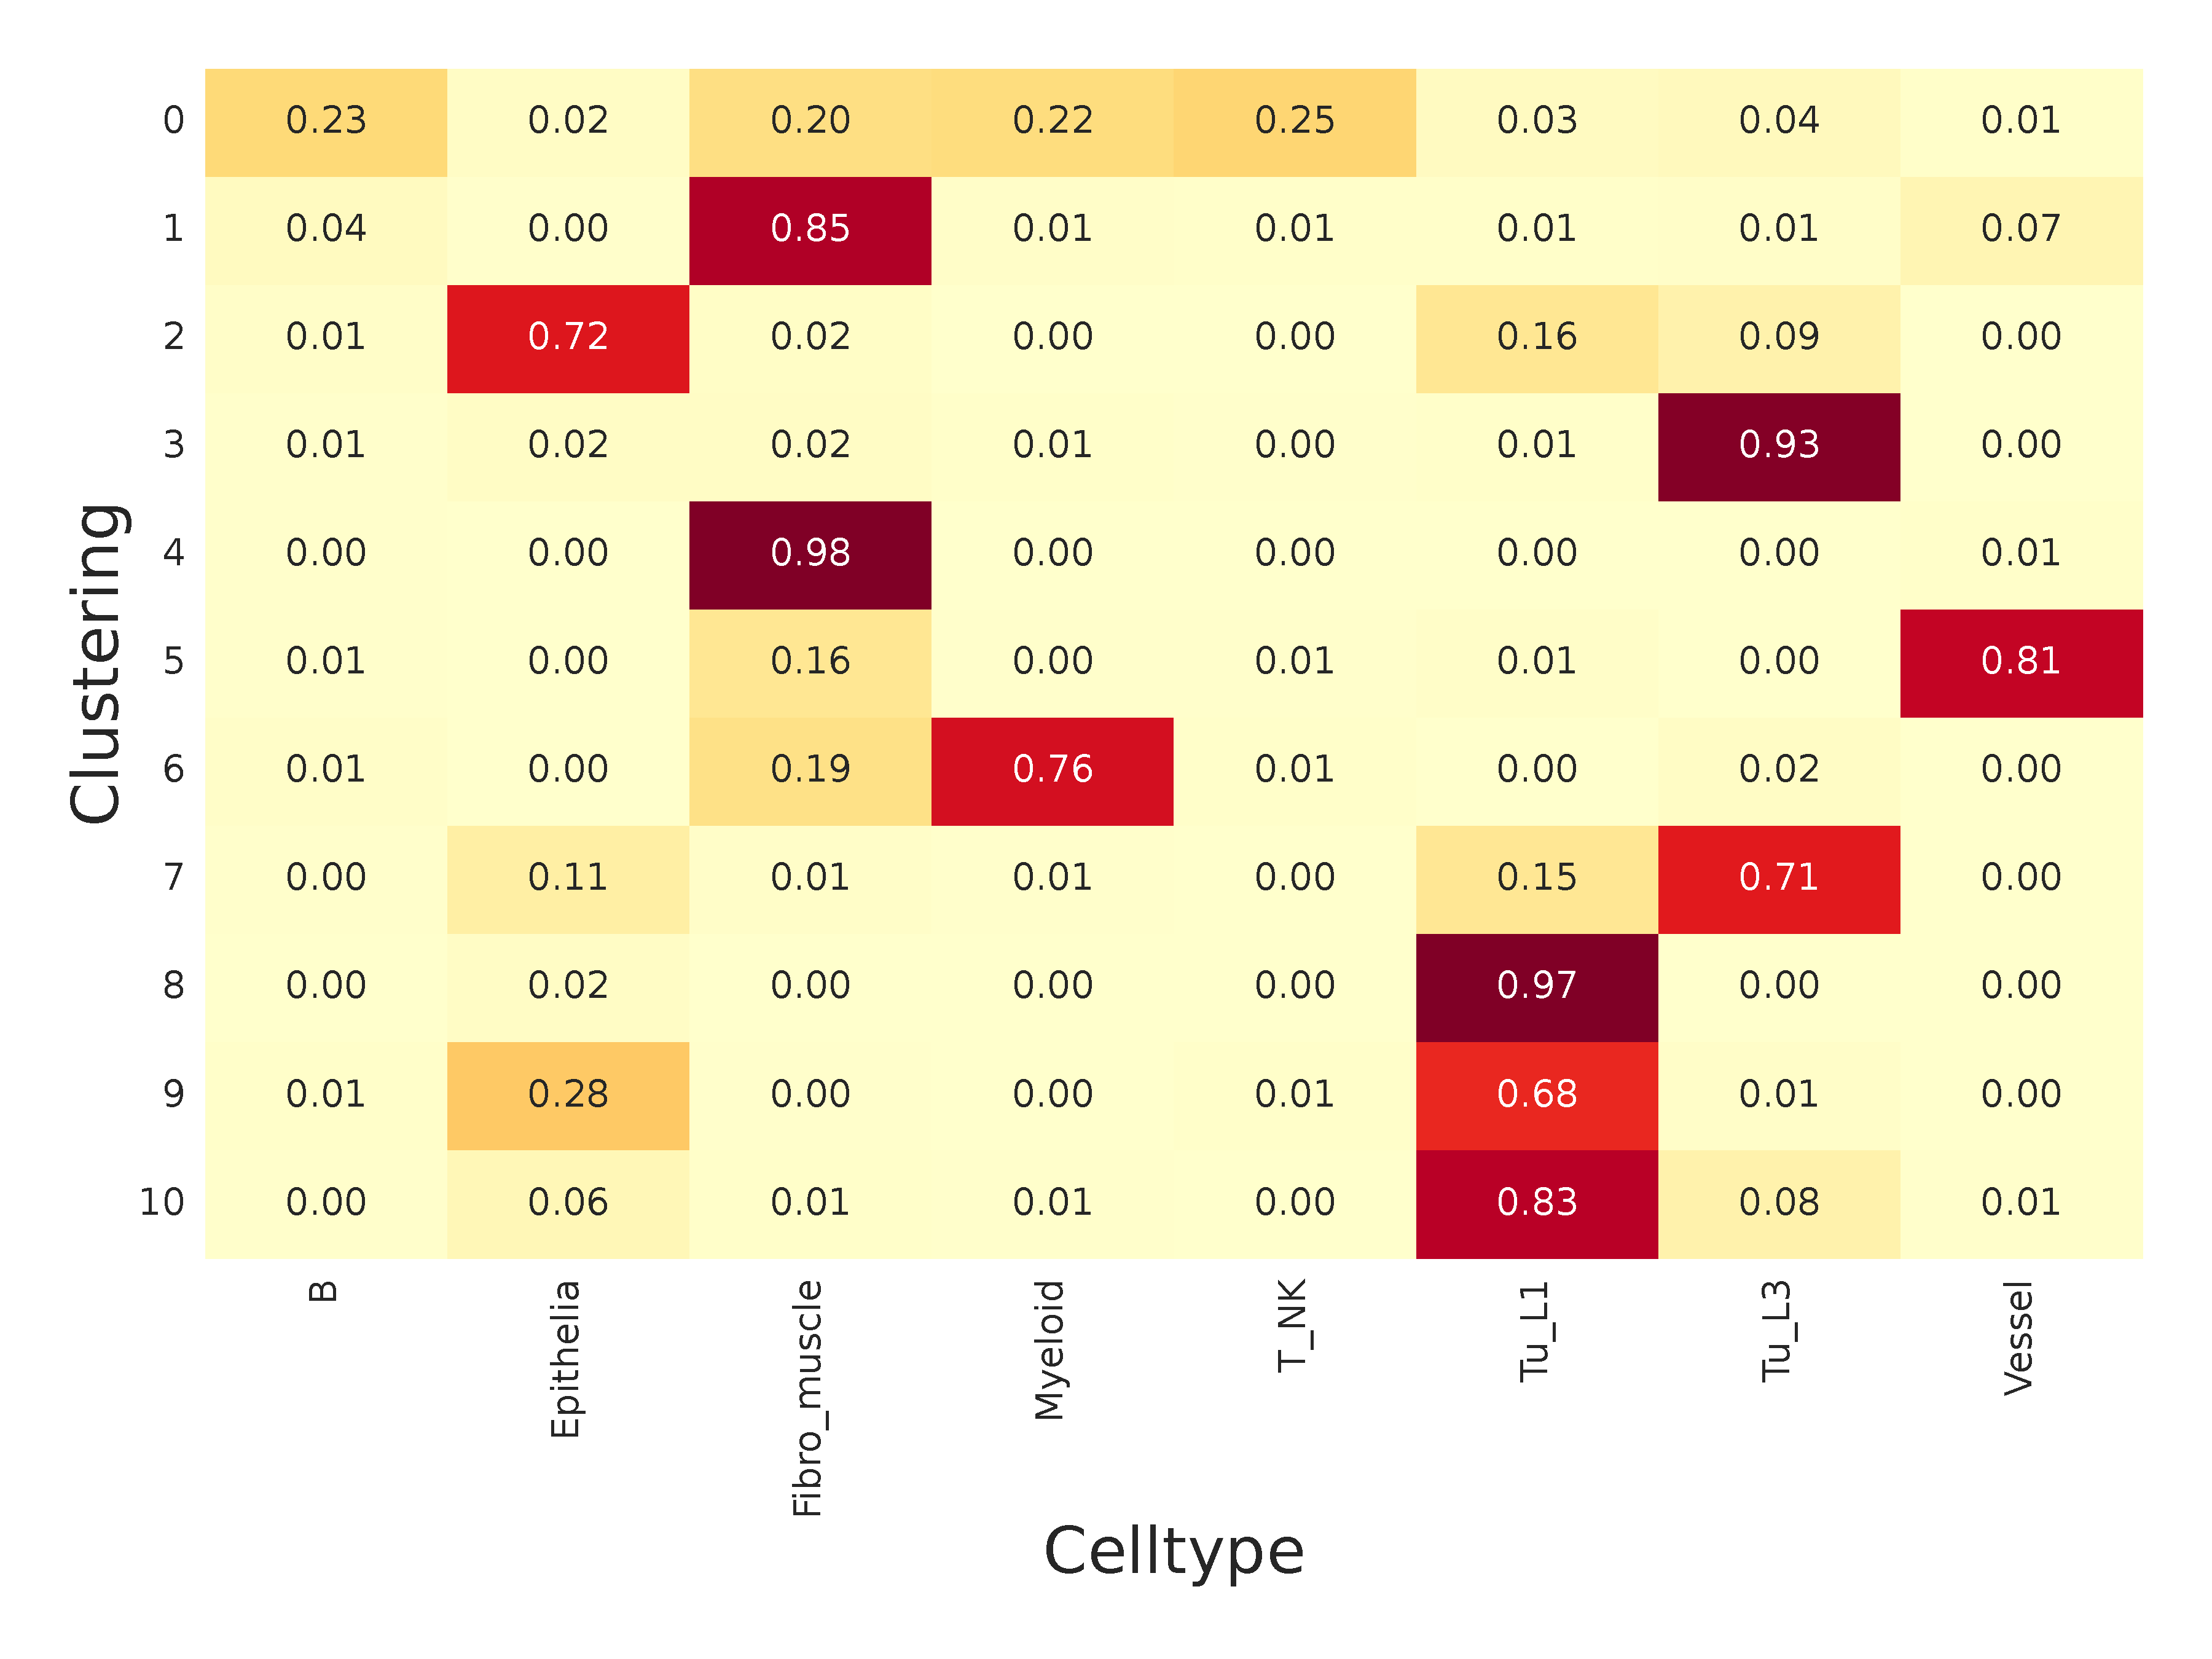
\includegraphics[width=\linewidth]{Figures/08_Marker_genes/Celltype-Proportion-Heatmap.pdf}
                    \caption{Relative proportion}
                \end{figure}
            \end{column}
        \end{columns}
    \end{frame}

    \subsection{Xenimum coordiantes}

    \section{References}
    \begin{frame}[allowframebreaks]
        \frametitle{References}
        \bibliographystyle{apacite}
        \bibliography{References}
    \end{frame}
\end{document}